\chapter{Testing e analisi}\label{ch:test_analysis}

Come detto in precedenza, ASCON propone tre famiglie di algoritmi crittografici: AEAD, funzioni hash e funzioni auth. Sono state testate tutte le famiglie proposte utilizzando diverse grandezze di plaintext e tre diversi dispositivi IoT fisici, ossia Arduino Due, Adafruit ItsyBitsy M0 Express e RaspberryPi model 3B. Le prime due board sono prive di sistema operativo, mentre l'ultima è stata utilizzata con la distribuzione ``Raspberry Pi OS''. \

\noindent In questo capitolo verranno usati i termini ``algoritmo'' per indicare un algoritmo di una data famiglia e ``implementazione'' per indicare un'implementazione di un dato algoritmo di una data famiglia. Viene fatto questo per evitare di ripetere ogni volta ``una data implementazione di un dato algoritmo di una data famiglia''.

\section{Suite di test}

Per poter partecipare alla gara del NIST, ASCON ha inserito nel proprio repository Github una serie di test che possono essere compilati ed eseguiti su ogni architettura supportata. I test forniti eseguivano mediamente mille esecuzioni di una implementazione scelta, usando di volta in volta diverse grandezze di plaintext e di dati associati. Il test utilizzato per i risultati presenti in questo report esegue al massimo nove esecuzioni per l'implementazione in esame, testando plaintext e dati associati di grandezze minime, massime – secondo i test definiti da ASCON – e intermedie significative.

\subsection{Pseudocodice}

\begin{algorithm}
    \caption{Testing con varie lunghezze di plaintext e dati associati.}
    \label{alg:testing}
    \begin{algorithmic}[1]
        \Require{Lunghezza $mlen$ del plaintext.}
        \Require{Lunghezza $adlen$ dei dati associati (solo AEAD).}

        \LComment{Generazione di chiave, nonce e dati associati.}
        \State $key \gets$ \Call{GENERATE\_KEY}{$klen$}
        \State $nonce \gets$ \Call{GENERATE\_NONCE}{$nlen$}
        \State $ad \gets$ \Call{GENERATE\_AD}{$adlen$}
        \State \phantom{}

        \LComment{Generazione del plaintext da testare.}
        \State $pt \gets$ \Call{GENERATE\_PT}{$mlen$}
        \State \phantom{}

        \LComment{Inizio timer.}
        \State $time \gets$ \Call{GET\_TIME}{}
        \State \phantom{}

        \LComment{Cifratura e misura del tempo di esecuzione.}
        \State $ct, error \gets$ \Call{ENCRYPT}{$pt, \, key, \, nonce, \, ad$}
        \State $time \gets$ \Call{GET\_TIME}{} - time
        \State \phantom{}

        \LComment{Controllo degli errori.}
        \If{$error > 0$}
            \State \Call{EXIT}{$error$}
        \EndIf
        \State \phantom{}

        \LComment{Stampa dei risultati.}
        \State \Call{PRINT}{$time$}
        \State \phantom{}

        \LComment{Se la famiglia testata è AEAD oppure autenticazione viene eseguita la funzione di check}
        \If{$family \in \{AEAD, autenticazione\}$}
            \LComment{Inizio timer.}
            \State $time \gets$ \Call{GET\_TIME}{}
            \State \phantom{}

            \LComment{Decifratura e misura del tempo di esecuzione.}
            \State $pt, error \gets$ \Call{DECRYPT}{$ct, \, key, \, nonce, \, ad$}
            \State $time \gets$ \Call{GET\_TIME}{} - time
            \State \phantom{}

            \LComment{Controllo degli errori.}
            \If{$error > 0$}
                \State \Call{EXIT}{$error$}
            \EndIf
            \State \phantom{}

            \LComment{Stampa dei risultati.}
            \State \Call{PRINT}{$time$}
        \EndIf
    \end{algorithmic}
\end{algorithm}

Lo \rif[pseudocodice]{alg:testing} (vedi sotto) mostra la funzione di test utilizzata, creata modificando leggermente quella fornita da ASCON per poter rilevare i tempi di esecuzione. Per avere dei dati consistenti, la funzione di test viene chiamata mille volte per ogni grandezza di plaintext e dati associati in esame.

\noindent Per inserire i risultati come righe di un file CSV facilmente interrogabili, il programma che richiama la funzione di test esegue per mille volte un loop, nel quale vengono usate in sequenza le varie grandezze di plaintext e dati associati, così da avere, per ogni riga del file CSV, i tempi di esecuzione di un campionamento sulle lunghezze da testare.

\begin{algorithm}
    \caption{Come viene chiamata la funzione di test.}
    \begin{algorithmic}[1]
        \LComment{Funzione di test.}
        \For{$\_ \text{ in } range(1000)$}
            \State \Call{TEST}{$mlen_1$, $adlen_1$}
            \State \dots
            \State \Call{TEST}{$mlen_{n-1}$, $adlen_{n-1}$}
			\State \Call{SEND\_RESULTS}{\empty}
        \EndFor
    \end{algorithmic}
\end{algorithm}

\noindent L'header di ogni file CSV è composto da celle nel formato ``\textit{NB-M}'', con:
\begin{itemize}
    \item \textit{N}: grandezza in byte del plaintext testato;
    \item \textit{B}: indica appunto che la grandezza $N$ è in byte;
    \item \textit{M}: modalità, che per AEAD può essere \textit{E} (\textit{encryption}) oppure \textit{D} (\textit{decryption}), per autenticazione può essere \textit{A} (\textit{authentication}) oppure \textit{V} (\textit{verify}) mentre per hash questo campo non è presente.
\end{itemize}

\begin{table}[H]
    \centering
	\begin{tabular}{|c|c|c|c|c|c|c|c|}
		\hline
		0B-E & 0B-D & 1B-E & 1B-D & 8B-E & 8B-D & 16B-E & 16B-D \\
		\hline
    \end{tabular}
    \caption{Header AEAD con plaintext da 0, 1 8 e 16 byte.}
\end{table}

\subsection{Compilazione}

Per le board prive di sistema operativo è stato utilizzato il software Arduino IDE: il file di test veniva dapprima inserito in un progetto Arduino con i file che definivano l'implementazione scelta, successivamente compilato tramite il compilatore presente nella suite Arduino e infine trasferito tramite porta seriale alla board sotto testing. Per quanto riguarda la board con il sistema operativo, il file di test e i file dell'implementazione scelta venivano messi in una cartella, trasferiti sulla board tramite l'utility \textit{scp}, compilati con \textit{gcc} e infine eseguiti.

\subsection{Raccolta dei risultati}

Per le due board prive di sistema operativo, i risultati delle mille esecuzioni dei test di varie grandezze di plaintext e dati associati vengono inviati sulla porta seriale e intercettati da uno script Python che li inserisce in file CSV.

\begin{python}
import argparse, os, serial
from serial import SerialException


def main(filename: str, port: str) -> None:
  while True:
    try:
      s = serial.Serial(port, 9600)
        break
      except SerialException:
        port = input("Porta errata da ARGV, inserisci la porta: ")

  files = [file.split(".")[0] for file in os.listdir()]
  while filename not in files:
    filename = input("Nome errato da ARGV, inserisci il nome: ")

  with open(f"{filename}.csv", "a") as f:
    for i in range(1000):
      f.write(f"{s.readline().strip().decode()}\n")


if __name__ == "__main__":
  parser = argparse.ArgumentParser()
  parser.add_argument("filename")
  parser.add_argument("port")

  args = parser.parse_args()
  main(args.filename, args.port)
\end{python}

\noindent Lo script presentato per mille iterazioni legge dalla porta seriale un'esecuzione del loop di test e scrive il record nel file CSV corrispondente. \\

\noindent Nella board con il sistema operativo la logica di raccolta dati è stata invece spostata dentro il programma di test, che quando rileva un tempo di esecuzione lo va a scrivere direttamente nel file CSV.

\newpage

\section{Dispositivi utilizzati}

L'attività di testing è stata eseguita su tre dispositivi IoT fisici: \textbf{Arduino Due}, \textbf{Adafruit ItsyBitsy M0 Express} e \textbf{RaspberryPi model 3B}.

\noindent Nei capitoli successivi saranno presenti due tipi di tabelle:
\begin{enumerate}[label=\Roman*.]
    \item \textbf{Tempi di esecuzione}: contengono, appunto, i tempi di esecuzione, raccolti per implementazione e algoritmo; queste tabelle sono organizzate nel seguente modo:
    \begin{itemize}
        \item Header: contiene celle nel formato ``\textit{N-V}'', dove:
        \begin{itemize}
            \item $N$: grandezza in byte del plaintext testato;
            \item $V$: tipo di valore indicato nelle celle sottostanti, e può essere:
            \begin{enumerate}[label=(\arabic*)]
                \item m: valore minimo;
                \item a: valore medio;
                \item M: valore massimo.
            \end{enumerate}
            \begin{table}[H]
                \centering
            	\begin{tabular}{|c|c|c|c|c|c|c|c|c|}
            		\hline
            		0-m & 0-a & 0-M & 1-m & 1-a & 1-M & 8-m & 8-a & 8-M \\
            		\hline
                \end{tabular}
                \caption{Header tabella con plaintext da 0, 1 e 8 byte.}
            \end{table}
        \end{itemize}
        \item Righe, che contengono:
            \begin{itemize}
                \item il nome dell'algoritmo da testare e una serie di colonne vuote, oppure
                \item il nome di una implementazione dell'algoritmo letto precedentemente e una serie di colonne che rappresentano i tempi di esecuzione raccolti, misurati in microsecondi.
            \end{itemize}
            \begin{table}[H]
                \centering
            	\begin{tabular}{|c|c|c|}
            		\hline
                    \texttt{ascon128av12} & & \\
                    \hline
                    \texttt{arvm6m} & \dots & \dots \\
                    \hline
                    \texttt{ref} & \dots & \dots \\
            		\hline
                \end{tabular}
                \caption{Righe tabella con algoritmo \texttt{ascon128av12} e implementazioni \texttt{armv6m} e \texttt{ref}.}
            \end{table}
    \end{itemize}
    \item \textbf{Spazio utilizzato}: contengono alcune informazioni sulle proprietà dei file eseguibili compilati. Per le due board prive di sistema operativo, queste informazioni sono state ricavate dal terminale dell'Arduino IDE, e sono le seguenti:
    \begin{itemize}
        \item Sketch: dimensione del file compilato in byte. È presente anche una percentuale, che indica quanto occupa lo sketch nella memoria della board;
        \item Eseguibile: dimensione del file compilato, al quale vengono aggiunti alcuni header per poter essere eseguito sulla board, sempre misurato in byte;
        \item Pagine: numero di pagine;
        \item Loading time: secondi impiegati per trasferire il file eseguibile dal dispositivo host alla board.
    \end{itemize}
    Per quanto riguarda invece la board con il sistema operativo, l'unica informazione disponibile è la grandezza in byte del file eseguibile, ricavata tramite l'utility \textit{stat}. La struttura delle righe è la stessa della tabella precedente.
\end{enumerate}

\noindent Per quanto riguarda le famiglie AEAD e auth, saranno presenti tre tabelle: (1) tempi di esecuzione durante la fase di cifratura/autenticazione ; (2) tempi di esecuzione durante la fase di decifratura/verifica; (3) spazio utilizzato. Invece, per la famiglia hash, sarà presente una sola tabella con i tempi di esecuzione delle funzioni prese in esame e la tabella dello spazio utilizzato.

\subsection{Adafruit ItsyBitsy M0 Express}

La prima board testata è un prodotto Adafruit con un processore 32 bit ATSAMD21G18 Cortex M0+ a 48 MHz, 256 KB di memoria flash e 32 KB di memoria RAM\cite{adafruit}. L'architettura della board è ARMv6-M, presente nelle ottimizzazioni fornite da ASCON\cite{arm}.

\subsubsection{Crypto AEAD}

Per la famiglia crypto AEAD sono stati testati tutti gli algoritmi proposti nelle seguenti implementazioni: \texttt{ARMv6-M}, \texttt{ARMv6-M lowsize}, \texttt{bi32}, \texttt{bi32 ARMv6-M}, \texttt{bi32 lowreg}, \texttt{bi32 lowsize}, \texttt{opt32}, \texttt{opt32 lowsize} e \texttt{ref}.

\begin{table}[h]
    \caption{Spazio utilizzato famiglia AEAD.}
    \centering
	\begin{tabular}{|c|c|c|c|c|}
		\hline
         & \textbf{Sketch} & \textbf{Eseguibile} & \textbf{Pagine} & \textbf{Loading time} \\
        \hline
        \texttt{\textbf{ascon128abi32}} & & & & \\
        \hline  
        \texttt{bi32} & 27760 [10\%] & 27852 & 436 & 0.239 \\
        \hline
        \texttt{bi32 armv6m} & 23116 [8\%] & 23208 & 363 & 0.200 \\
        \hline
        \texttt{bi32 lowreg} & 21140 [8\%] & 21232 & 332 & 0.189 \\
        \hline
        \texttt{bi32 lowsize} & 16928 [6\%] & 17020 & 266 & 0.136 \\
        \hline
        \texttt{ref} & 48352 [18\%] & 48444 & 757 & 0.448 \\
        \hline
        \texttt{\textbf{ascon128av12}} & & & & \\
        \hline
        \texttt{armv6m} & 23108 [8\%] & 23200 & 363 & 0.210 \\
        \hline
        \texttt{armv6m lowsize} & 16888 [6\%] & 16980 & 266 & 0.179 \\
        \hline
        \texttt{bi32} & 32132 [12\%] & 32224 & 504 & 0.300 \\
        \hline
        \texttt{bi32 armv6m} & 27748 [10\%] & 27840 & 435 & 0.271 \\
        \hline
        \texttt{bi32 lowreg} & 24964 [9\%] & 25056 & 391 & 0.240 \\
        \hline
        \texttt{bi32 lowsize} & 16600 [6\%] & 16692 & 261 & 0.164 \\
        \hline
        \texttt{opt32} & 58872 [22\%] & 58964 & 922 & 0.455 \\
        \hline
        \texttt{opt32 lowsize} & 16972 [6\%] & 17064 & 267 & 0.170 \\
        \hline
        \texttt{ref} & 56412 [21\%] & 56504 & 883 & 0.526 \\
        \hline
        \texttt{\textbf{ascon128bi32v12}} & & & & \\
        \hline
        \texttt{bi32} & 25824 [9\%] & 25916 & 405 & 0.201 \\
        \hline
        \texttt{bi32 armv6m} & 21916 [8\%] & 22008 & 344 & 0.198 \\
        \hline
        \texttt{bi32 lowreg} & 20232 [7\%] & 20324 & 318 & 0.155 \\
        \hline
        \texttt{bi32 lowsize} & 16864 [6\%] & 16956 & 265 & 0.185 \\
        \hline
        \texttt{ref} & 39628 [15\%] & 39720 & 621 & 0.370 \\
        \hline
        \texttt{\textbf{ascon128v12}} & & & & \\
        \hline
        \texttt{armv6m} & 21864 [8\%] & 21956 & 344 & 0.227 \\
        \hline
        \texttt{armv6m lowsize} & 16824 [6\%] & 16916 & 265 & 0.183 \\
        \hline
        \texttt{bi32} & 28736 [10\%] & 28828 & 451 & 0.369 \\
        \hline
        \texttt{bi32 armv6m} & 25076 [9\%] & 25168 & 394 & 0.249 \\
        \hline
        \texttt{bi32 lowreg} & 22880 [8\%] & 22972 & 359 & 0.192 \\
        \hline
        \texttt{bi32 lowsize} & 16560 [6\%] & 16652 & 261 & 0.159 \\
        \hline
        \texttt{opt32} & 52768 [20\%] & 52860 & 826 & 0.425 \\
        \hline
        \texttt{opt32 lowsize} & 16908 [6\%] & 17000 & 266 & 0.170 \\
        \hline
        \texttt{ref} & 53044 [20\%] & 53136 & 831 & 0.484 \\
        \hline
    \end{tabular}
\end{table}

\begin{landscape}
    \begin{table}[]
        \caption{Prestazioni famiglia crypto AEAD nella fase di cifratura.}
        \begin{adjustbox}{width=600pt}
            \centering
			\begin{tabular}{|c|c|c|c|c|c|c|c|c|c|c|c|c|c|c|c|c|c|c|}
				\hline
				& \textbf{0-m} & \textbf{0-a} & \textbf{0-M} & \textbf{1-m} & \textbf{1-a} & \textbf{1-M} & \textbf{16-m} & \textbf{16-a} & \textbf{16-M} & \textbf{32-m} & \textbf{32-a} & \textbf{32-M} & \textbf{48-m} & \textbf{48-a} & \textbf{48-M} & \textbf{64-m} & \textbf{64-a} & \textbf{64-M} \\
				\hline
				\texttt{\textbf{ascon128av12}} & & & & & & & & & & & & & & & & & & \\
				\hline
				\texttt{armv6m} & 121 & 122.46 & 130 & 163 & 164.85 & 172 & 236 & 239.09 & 245 & 315 & 317.96 & 325 & 393 & 396.3 & 404 & 471 & 475.99 & 482 \\
				\hline
				\texttt{armv6m lowsize} & 129 & 130.73 & 138 & 171 & 172.9 & 180 & 255 & 258.27 & 266 & 341 & 344.3 & 352 & 426 & 430.77 & 437 & 511 & 516.54 & 522 \\
				\hline
				\texttt{bi32} & 186 & 187.82 & 196 & 249 & 251.8 & 260 & 364 & 367.39 & 374 & 487 & 492.29 & 498 & 611 & 617.51 & 622 & 735 & 742.61 & 746 \\
				\hline
				\texttt{bi32 armv6m} & 129 & 130.34 & 138 & 176 & 177.42 & 184 & 252 & 254.79 & 261 & 339 & 342.34 & 348 & 426 & 430.32 & 437 & 512 & 517.65 & 523 \\
				\hline
				\texttt{bi32 lowreg} & 207 & 209.28 & 218 & 271 & 274.46 & 282 & 382 & 385.86 & 393 & 504 & 509.15 & 515 & 626 & 632.08 & 637 & 748 & 755.4 & 759 \\
				\hline
				\texttt{bi32 lowsize} & 197 & 199.71 & 208 & 257 & 259.81 & 267 & 386 & 390.48 & 397 & 516 & 520.78 & 527 & 646 & 652.12 & 657 & 776 & 783.53 & 786 \\
				\hline
				\texttt{opt32} & 155 & 156.86 & 163 & 207 & 209.17 & 217 & 308 & 311.21 & 318 & 413 & 417.96 & 424 & 519 & 524.11 & 530 & 625 & 630.99 & 636 \\
				\hline
				\texttt{opt32 lowsize} & 202 & 204.38 & 211 & 267 & 269.48 & 277 & 399 & 402.76 & 409 & 531 & 536.5 & 542 & 664 & 670.81 & 675 & 799 & 804.17 & 808 \\
				\hline
				\texttt{ref} & 173 & 174.24 & 183 & 224 & 226.88 & 235 & 347 & 351.0 & 358 & 472 & 477.07 & 483 & 596 & 602.63 & 607 & 721 & 727.8 & 732 \\
				\hline
				\texttt{\textbf{ascon128abi32v12}} & & & & & & & & & & & & & & & & & & \\
				\hline
				\texttt{bi32} & 176 & 177.9 & 184 & 235 & 237.24 & 243 & 344 & 347.1 & 352 & 457 & 461.65 & 468 & 571 & 576.1 & 581 & 686 & 690.7 & 695 \\
				\hline
				\texttt{bi32 armv6m} & 118 & 119.44 & 127 & 159 & 160.77 & 168 & 231 & 233.6 & 240 & 308 & 310.16 & 318 & 384 & 388.43 & 395 & 460 & 464.19 & 471 \\
				\hline
				\texttt{bi32 lowreg} & 194 & 196.44 & 203 & 253 & 255.83 & 262 & 359 & 362.72 & 369 & 470 & 474.73 & 481 & 581 & 587.03 & 592 & 694 & 698.73 & 703 \\
				\hline
				\texttt{bi32 lowsize} & 182 & 183.78 & 192 & 240 & 242.75 & 251 & 358 & 362.15 & 369 & 477 & 482.16 & 488 & 596 & 602.59 & 607 & 715 & 722.22 & 726 \\
				\hline
				\texttt{ref} & 169 & 170.85 & 180 & 217 & 220.13 & 228 & 334 & 337.24 & 345 & 452 & 456.87 & 462 & 570 & 575.46 & 580 & 687 & 694.38 & 698 \\
				\hline
				\texttt{\textbf{ascon128v12}} & & & & & & & & & & & & & & & & & & \\
				\hline
				\texttt{armv6m} & 119 & 119.91 & 128 & 152 & 152.96 & 160 & 206 & 207.83 & 216 & 265 & 267.73 & 275 & 324 & 327.1 & 334 & 382 & 386.09 & 393 \\
				\hline
				\texttt{armv6m lowsize} & 129 & 130.48 & 138 & 162 & 163.48 & 170 & 223 & 224.77 & 231 & 284 & 286.56 & 293 & 345 & 348.7 & 356 & 407 & 410.7 & 417 \\
				\hline
				\texttt{bi32} & 185 & 187.27 & 194 & 238 & 240.12 & 248 & 321 & 324.33 & 332 & 413 & 417.65 & 424 & 506 & 510.69 & 517 & 598 & 604.42 & 610 \\
				\hline
				\texttt{bi32 armv6m} & 127 & 128.23 & 136 & 166 & 167.29 & 174 & 218 & 220.3 & 227 & 281 & 284.24 & 290 & 344 & 348.01 & 353 & 407 & 411.71 & 416 \\
				\hline
				\texttt{bi32 lowreg} & 206 & 208.68 & 215 & 258 & 261.17 & 267 & 336 & 339.26 & 345 & 424 & 429.12 & 435 & 513 & 518.39 & 525 & 602 & 608.64 & 613 \\
				\hline
				\texttt{bi32 lowsize} & 197 & 199.01 & 208 & 244 & 245.92 & 254 & 334 & 337.56 & 345 & 425 & 429.63 & 436 & 517 & 521.86 & 527 & 608 & 613.94 & 619 \\
				\hline
				\texttt{opt32} & 158 & 160.28 & 167 & 200 & 201.95 & 209 & 273 & 275.89 & 282 & 351 & 354.1 & 361 & 429 & 433.07 & 439 & 506 & 511.35 & 517 \\
				\hline
				\texttt{opt32 lowsize} & 202 & 203.93 & 211 & 252 & 254.35 & 263 & 347 & 350.82 & 358 & 443 & 447.6 & 454 & 539 & 544.58 & 550 & 635 & 641.72 & 646 \\
				\hline
				\texttt{ref} & 173 & 175.03 & 182 & 213 & 214.88 & 223 & 299 & 301.88 & 309 & 386 & 389.68 & 397 & 473 & 478.02 & 484 & 561 & 566.73 & 572 \\
				\hline
				\texttt{\textbf{ascon128bi32v12}} & & & & & & & & & & & & & & & & & & \\
				\hline
				\texttt{bi32} & 175 & 177.36 & 184 & 222 & 224.83 & 231 & 305 & 308.18 & 314 & 392 & 395.9 & 402 & 479 & 483.62 & 490 & 566 & 571.93 & 577 \\
				\hline
				\texttt{bi32 armv6m} & 116 & 117.35 & 125 & 149 & 150.77 & 158 & 203 & 204.77 & 212 & 261 & 263.84 & 270 & 319 & 322.32 & 329 & 376 & 380.52 & 387 \\
				\hline
				\texttt{bi32 lowreg} & 194 & 196.2 & 205 & 240 & 242.17 & 250 & 317 & 320.03 & 328 & 399 & 402.93 & 410 & 481 & 485.95 & 492 & 564 & 569.21 & 574 \\
				\hline
				\texttt{bi32 lowsize} & 181 & 183.66 & 192 & 226 & 228.98 & 237 & 311 & 314.72 & 322 & 397 & 401.58 & 408 & 483 & 487.69 & 494 & 569 & 574.31 & 580 \\
				\hline
				\texttt{ref} & 176 & 178.07 & 185 & 222 & 224.08 & 231 & 303 & 306.25 & 312 & 385 & 389.05 & 394 & 467 & 472.0 & 478 & 552 & 555.67 & 561 \\
				\hline
			\end{tabular}
		\end{adjustbox}
	\end{table}
\end{landscape}

\begin{landscape}
    \begin{table}[]
        \caption{Prestazioni famiglia crypto AEAD nella fase di decifratura.}
        \begin{adjustbox}{width=600pt}
            \centering
			\begin{tabular}{|c|c|c|c|c|c|c|c|c|c|c|c|c|c|c|c|c|c|c|}
				\hline
				& \textbf{0-m} & \textbf{0-a} & \textbf{0-M} & \textbf{1-m} & \textbf{1-a} & \textbf{1-M} & \textbf{16-m} & \textbf{16-a} & \textbf{16-M} & \textbf{32-m} & \textbf{32-a} & \textbf{32-M} & \textbf{48-m} & \textbf{48-a} & \textbf{48-M} & \textbf{64-m} & \textbf{64-a} & \textbf{64-M} \\
				\hline
				\texttt{\textbf{ascon128av12}} & & & & & & & & & & & & & & & & & & \\
				\hline
				\texttt{armv6m} & 244 & 246.76 & 253 & 331 & 334.71 & 342 & 480 & 484.84 & 491 & 641 & 646.86 & 652 & 804 & 809.86 & 813 & 965 & 971.95 & 974 \\
				\hline
				\texttt{armv6m lowsize} & 264 & 266.93 & 275 & 348 & 351.13 & 358 & 522 & 526.66 & 533 & 698 & 704.47 & 709 & 876 & 882.0 & 885 & 1059 & 1059.62 & 1062 \\
				\hline
				\texttt{bi32} & 373 & 376.49 & 384 & 503 & 507.41 & 513 & 732 & 739.08 & 743 & 985 & 991.8 & 994 & 1242 & 1244.72 & 1253 & 1493 & 1497.68 & 1504 \\
				\hline
				\texttt{bi32 armv6m} & 261 & 263.25 & 270 & 357 & 360.33 & 365 & 512 & 516.57 & 522 & 692 & 696.95 & 701 & 871 & 877.28 & 880 & 1057 & 1057.45 & 1060 \\
				\hline
				\texttt{bi32 lowreg} & 415 & 418.47 & 426 & 546 & 551.19 & 557 & 772 & 778.91 & 783 & 1031 & 1031.59 & 1035 & 1281 & 1284.24 & 1292 & 1531 & 1536.18 & 1542 \\
				\hline
				\texttt{bi32 lowsize} & 399 & 402.28 & 409 & 519 & 523.84 & 530 & 782 & 789.65 & 793 & 1056 & 1056.76 & 1060 & 1321 & 1324.22 & 1332 & 1586 & 1591.94 & 1597 \\
				\hline
				\texttt{opt32} & 320 & 323.21 & 331 & 427 & 430.84 & 438 & 631 & 636.51 & 642 & 849 & 854.99 & 858 & 1072 & 1073.18 & 1081 & 1289 & 1291.63 & 1299 \\
				\hline
				\texttt{opt32 lowsize} & 409 & 412.92 & 420 & 540 & 544.47 & 550 & 811 & 816.14 & 820 & 1089 & 1089.3 & 1097 & 1359 & 1362.71 & 1370 & 1630 & 1636.17 & 1641 \\
				\hline
				\texttt{ref} & 368 & 371.86 & 379 & 473 & 477.56 & 484 & 724 & 730.67 & 735 & 981 & 988.0 & 990 & 1242 & 1245.12 & 1254 & 1497 & 1501.84 & 1508 \\
				\hline
				\texttt{\textbf{ascon128abi32v12}} & & & & & & & & & & & & & & & & & & \\
				\hline
				\texttt{bi32} & 353 & 356.6 & 362 & 474 & 478.85 & 485 & 695 & 699.53 & 704 & 926 & 933.04 & 935 & 1165 & 1166.14 & 1174 & 1396 & 1399.85 & 1405 \\
				\hline
				\texttt{bi32 armv6m} & 237 & 240.22 & 246 & 323 & 326.41 & 332 & 469 & 472.22 & 480 & 627 & 632.54 & 637 & 786 & 791.14 & 795 & 944 & 950.23 & 953 \\
				\hline
				\texttt{bi32 lowreg} & 390 & 394.12 & 401 & 511 & 515.64 & 522 & 728 & 732.76 & 737 & 955 & 962.06 & 964 & 1190 & 1191.97 & 1199 & 1418 & 1421.48 & 1428 \\
				\hline
				\texttt{bi32 lowsize} & 369 & 372.0 & 379 & 486 & 490.18 & 496 & 727 & 733.87 & 738 & 971 & 979.84 & 982 & 1223 & 1225.64 & 1234 & 1466 & 1471.25 & 1477 \\
				\hline
				\texttt{ref} & 386 & 389.56 & 397 & 484 & 488.69 & 495 & 720 & 727.09 & 731 & 961 & 970.12 & 972 & 1210 & 1212.37 & 1221 & 1450 & 1454.99 & 1461 \\
				\hline
				\texttt{\textbf{ascon128v12}} & & & & & & & & & & & & & & & & & & \\
				\hline
				\texttt{armv6m} & 241 & 242.96 & 251 & 309 & 311.37 & 320 & 418 & 421.92 & 428 & 538 & 542.79 & 549 & 658 & 664.36 & 669 & 778 & 785.87 & 789 \\
				\hline
				\texttt{armv6m lowsize} & 263 & 266.14 & 272 & 329 & 332.54 & 338 & 453 & 456.58 & 463 & 578 & 583.31 & 589 & 705 & 709.77 & 714 & 830 & 836.0 & 839 \\
				\hline
				\texttt{bi32} & 373 & 375.86 & 383 & 478 & 482.34 & 489 & 645 & 650.52 & 656 & 835 & 840.92 & 844 & 1029 & 1030.15 & 1033 & 1217 & 1219.24 & 1226 \\
				\hline
				\texttt{bi32 armv6m} & 256 & 258.9 & 265 & 335 & 338.53 & 344 & 441 & 445.68 & 450 & 570 & 575.69 & 581 & 701 & 705.66 & 710 & 830 & 835.4 & 839 \\
				\hline
				\texttt{bi32 lowreg} & 414 & 417.52 & 425 & 520 & 524.78 & 531 & 674 & 678.71 & 683 & 852 & 858.27 & 861 & 1037 & 1037.89 & 1041 & 1215 & 1217.31 & 1224 \\
				\hline
				\texttt{bi32 lowsize} & 398 & 401.72 & 409 & 492 & 496.51 & 503 & 676 & 681.58 & 686 & 861 & 868.42 & 872 & 1055 & 1055.6 & 1058 & 1240 & 1242.57 & 1251 \\
				\hline
				\texttt{opt32} & 317 & 319.81 & 325 & 405 & 408.72 & 416 & 550 & 554.86 & 561 & 708 & 712.77 & 717 & 865 & 870.73 & 873 & 1028 & 1028.66 & 1032 \\
				\hline
				\texttt{opt32 lowsize} & 408 & 412.5 & 419 & 509 & 514.05 & 520 & 702 & 709.07 & 713 & 899 & 905.36 & 908 & 1101 & 1101.66 & 1109 & 1295 & 1298.48 & 1306 \\
				\hline
				\texttt{ref} & 361 & 364.81 & 372 & 442 & 446.24 & 453 & 616 & 622.23 & 627 & 794 & 801.06 & 805 & 973 & 980.17 & 982 & 1158 & 1159.81 & 1167 \\
				\hline
				\texttt{\textbf{ascon128bi32v12}} & & & & & & & & & & & & & & & & & & \\
				\hline
				\texttt{bi32} & 353 & 356.3 & 363 & 450 & 454.32 & 461 & 615 & 621.38 & 626 & 794 & 799.64 & 803 & 971 & 977.84 & 980 & 1155 & 1156.61 & 1164 \\
				\hline
				\texttt{bi32 armv6m} & 235 & 236.72 & 244 & 303 & 306.28 & 312 & 410 & 413.97 & 421 & 528 & 533.4 & 539 & 647 & 652.95 & 658 & 768 & 773.32 & 777 \\
				\hline
				\texttt{bi32 lowreg} & 390 & 393.85 & 401 & 484 & 488.62 & 495 & 638 & 644.39 & 649 & 805 & 812.86 & 816 & 974 & 981.16 & 983 & 1148 & 1149.88 & 1159 \\
				\hline
				\texttt{bi32 lowsize} & 368 & 370.92 & 378 & 458 & 462.45 & 469 & 631 & 636.55 & 641 & 805 & 812.45 & 815 & 981 & 987.71 & 990 & 1162 & 1163.54 & 1173 \\
				\hline
				\texttt{ref} & 372 & 375.09 & 381 & 464 & 468.59 & 475 & 628 & 631.9 & 637 & 793 & 798.76 & 802 & 959 & 965.53 & 968 & 1131 & 1132.69 & 1140 \\
				\hline
			\end{tabular}
		\end{adjustbox}
	\end{table}
\end{landscape}

\subsubsection{Crypto hash}

Per la famiglia crypto hash sono stati testati tutti gli algoritmi proposti nelle seguenti implementazioni: \texttt{ARMv6-M}, \texttt{ARMv6-M lowsize}, \texttt{bi32}, \texttt{bi32 ARMv6-M}, \texttt{bi32 lowreg}, \texttt{bi32 lowsize}, \texttt{opt32}, \texttt{opt32 lowsize} e \texttt{ref}.

\begin{table}[h]
    \caption{Spazio utilizzato famiglia hash.}
    \centering
    \begin{adjustbox}{width=207pt}
	\begin{tabular}{|c|c|c|c|c|}
		\hline
         & \textbf{Sketch} & \textbf{Eseguibile} & \textbf{Pagine} & \textbf{Loading time} \\
        \hline
        \texttt{\textbf{asconhashabi32v12}} & & & & \\
        \hline
        \texttt{bi32} & 23516 [8\%] & 23608 & 369 & 0.186 \\
        \hline
        \texttt{bi32 armv6m} & 16356 [6\%] & 16448 & 257 & 0.145 \\
        \hline
        \texttt{bi32 lowreg} & 16412 [6\%] & 16504 & 258 & 0.141 \\
        \hline
        \texttt{bi32 lowsize} & 15572 [5\%] & 15664 & 245 & 0.141 \\
        \hline
        \texttt{ref} & 27256 [10\%] & 27348 & 428 & 0.235 \\
        \hline
        \texttt{\textbf{asconhashav12}} & & & & \\
        \hline
        \texttt{armv6m} & 16332 [6\%] & 16424 & 257 & 0.153 \\
        \hline
        \texttt{armv6m lowsize} & 15540 [5\%] & 15632 & 245 & 0.147 \\
        \hline
        \texttt{bi32} & 24016 [9\%] & 24108 & 377 & 0.195 \\
        \hline
        \texttt{bi32 armv6m} & 16832 [6\%] & 16924 & 265 & 0.143 \\
        \hline
        \texttt{bi32 lowreg} & 16896 [6\%] & 16988 & 266 & 0.152 \\
        \hline
        \texttt{bi32 lowsize} & 15644 [5\%] & 15736 & 246 & 0.124 \\
        \hline
        \texttt{opt32} & 27028 [10\%] & 27120 & 424 & 0.218 \\
        \hline
        \texttt{opt32 lowsize} & 15628 [5\%] & 15720 & 246 & 0.126 \\
        \hline
        \texttt{ref} & 31836 [12\%] & 31928 & 499 & 0.256 \\
        \hline
        \texttt{\textbf{asconhashbi32v12}} & & & & \\
        \hline
        \texttt{bi32} & 20188 [7\%] & 20280 & 317 & 0.181 \\
        \hline
        \texttt{bi32 armv6m} & 16356 [6\%] & 16448 & 257 & 0.148 \\
        \hline
        \texttt{bi32 lowreg} & 16412 [6\%] & 16504 & 258 & 0.148 \\
        \hline
        \texttt{bi32 lowsize} & 15572 [5\%] & 15664 & 245 & 0.129 \\
        \hline
        \texttt{ref} & 27436 [10\%] & 27528 & 431 & 0.239 \\
        \hline
        \texttt{\textbf{asconhashv12}} & & & & \\
        \hline
        \texttt{armv6m} & 16332 [6\%] & 16424 & 257 & 0.172 \\
        \hline
        \texttt{armv6m lowsize} & 15540 [5\%] & 15632 & 245 & 0.154 \\
        \hline
        \texttt{bi32} & 20688 [7\%] & 20780 & 325 & 0.182 \\
        \hline
        \texttt{bi32 armv6m} & 16832 [6\%] & 16924 & 265 & 0.163 \\
        \hline
        \texttt{bi32 lowreg} & 16896 [6\%] & 16988 & 266 & 0.144 \\
        \hline
        \texttt{bi32 lowsize} & 15644 [5\%] & 15736 & 246 & 0.137 \\
        \hline
        \texttt{opt32} & 30500 [11\%] & 30592 & 478 & 0.261 \\
        \hline
        \texttt{opt32 lowsize} & 15628 [5\%] & 15720 & 246 & 0.128 \\
        \hline
        \texttt{ref} & 35384 [13\%] & 35476 & 555 & 0.298 \\
        \hline
        \texttt{\textbf{asconxofav12}} & & & & \\
        \hline
        \texttt{armv6m} & 16332 [6\%] & 16424 & 257 & 0.130 \\
        \hline
        \texttt{armv6m lowsize} & 15540 [5\%] & 15632 & 245 & 0.147 \\
        \hline
        \texttt{bi32} & 24016 [9\%] & 24108 & 377 & 0.212 \\
        \hline
        \texttt{bi32 armv6m} & 16832 [6\%] & 16924 & 265 & 0.147 \\
        \hline
        \texttt{bi32 lowreg} & 16896 [6\%] & 16988 & 266 & 0.137 \\
        \hline
        \texttt{bi32 lowsize} & 15644 [5\%] & 15736 & 246 & 0.131 \\
        \hline
        \texttt{opt32} & 27028 [10\%] & 27120 & 424 & 0.230 \\
        \hline
        \texttt{opt32 lowsize} & 15628 [5\%] & 15720 & 246 & 0.138 \\
        \hline
        \texttt{ref} & 31828 [12\%] & 31920 & 499 & 0.263 \\
        \hline
        \texttt{\textbf{asconxofv12}} & & & & \\
        \hline
        \texttt{armv6m} & 16332 [6\%] & 16424 & 257 & 0.161 \\
        \hline
        \texttt{armv6m lowsize} & 15540 [5\%] & 15632 & 245 & 0.179 \\
        \hline
        \texttt{bi32} & 20688 [7\%] & 20780 & 325 & 0.179 \\
        \hline
        \texttt{bi32 armv6m} & 16832 [6\%] & 16924 & 265 & 0.166 \\
        \hline
        \texttt{bi32 lowreg} & 16896 [6\%] & 16988 & 266 & 0.144 \\
        \hline
        \texttt{bi32 lowsize} & 15644 [5\%] & 15736 & 246 & 0.141 \\
        \hline
        \texttt{opt32} & 30500 [11\%] & 30592 & 478 & 0.246 \\
        \hline
        \texttt{opt32 lowsize} & 15628 [5\%] & 15720 & 246 & 0.137 \\
        \hline
        \texttt{ref} & 35340 [13\%] & 35432 & 554 & 0.286 \\
        \hline
    \end{tabular}
    \end{adjustbox}
\end{table}

\begin{landscape}
    \begin{table}[]
        \caption{Prestazioni famiglia hash.}
        \begin{adjustbox}{width=600pt}
            \centering
			\begin{tabular}{|c|c|c|c|c|c|c|c|c|c|c|c|c|c|c|c|c|c|c|c|c|c|c|c|c|c|c|c|}
				\hline
				& \textbf{0-m} & \textbf{0-a} & \textbf{0-M }& \textbf{8-m} & \textbf{8-a} & \textbf{8-M} & \textbf{16-m} & \textbf{16-a} & \textbf{16-M} & \textbf{32-m} & \textbf{32-a} & \textbf{32-M} & \textbf{64-m} & \textbf{64-a} & \textbf{64-M} & \textbf{128-m} & \textbf{128-a} & \textbf{128-M} & \textbf{256-m} & \textbf{256-a} & \textbf{256-M} & \textbf{512-m} & \textbf{512-a} & \textbf{512-M} & \textbf{1024-m} & \textbf{1024-a} & \textbf{1024-M} \\
				\hline
				\texttt{\textbf{asconhashav12}} & & & & & & & & & & & & & & & & & & & & & & & & & & & \\
				\hline
				\texttt{armv6m} & 184 & 186.0 & 195 & 222 & 223.19 & 232 & 259 & 261.34 & 270 & 333 & 338.34 & 344 & 481 & 484.63 & 492 & 778 & 786.73 & 789 & 1381 & 1383.88 & 1392 & 2577 & 2581.2 & 2588 & 4972 & 4979.65 & 4981 \\
				\hline
				\texttt{armv6m lowsize} & 187 & 189.2 & 199 & 225 & 227.58 & 236 & 263 & 265.76 & 274 & 339 & 342.69 & 350 & 492 & 496.62 & 503 & 796 & 803.51 & 807 & 1414 & 1418.29 & 1425 & 2641 & 2648.13 & 2652 & 5103 & 5106.19 & 5115 \\
				\hline
				\texttt{bi32} & 270 & 272.77 & 280 & 326 & 329.63 & 337 & 383 & 387.04 & 394 & 496 & 500.77 & 507 & 722 & 729.63 & 733 & 1184 & 1186.26 & 1194 & 2099 & 2099.95 & 2107 & 3920 & 3926.98 & 3929 & 7576 & 7581.98 & 7587 \\
				\hline
				\texttt{bi32 armv6m} & 191 & 192.45 & 200 & 229 & 231.61 & 238 & 267 & 269.46 & 277 & 343 & 347.73 & 354 & 496 & 501.29 & 507 & 803 & 808.88 & 812 & 1421 & 1425.93 & 1432 & 2652 & 2658.86 & 2663 & 5122 & 5124.35 & 5131 \\
				\hline
				\texttt{bi32 lowreg} & 271 & 272.83 & 280 & 327 & 330.86 & 336 & 382 & 386.51 & 391 & 494 & 498.72 & 504 & 718 & 722.61 & 727 & 1171 & 1172.64 & 1180 & 2071 & 2072.02 & 2080 & 3863 & 3870.66 & 3872 & 7460 & 7465.74 & 7471 \\
				\hline
				\texttt{bi32 lowsize} & 273 & 275.72 & 282 & 329 & 332.37 & 338 & 386 & 389.6 & 396 & 499 & 503.08 & 509 & 726 & 731.96 & 735 & 1185 & 1187.48 & 1194 & 2098 & 2099.39 & 2107 & 3916 & 3923.37 & 3925 & 7566 & 7571.58 & 7576 \\
				\hline
				\texttt{opt32} & 244 & 247.06 & 253 & 294 & 297.45 & 303 & 344 & 347.69 & 353 & 444 & 448.93 & 455 & 646 & 650.65 & 655 & 1053 & 1053.79 & 1062 & 1855 & 1861.51 & 1864 & 3470 & 3475.21 & 3481 & 6698 & 6703.58 & 6708 \\
				\hline
				\texttt{opt32 lowsize} & 294 & 297.51 & 303 & 356 & 359.31 & 365 & 418 & 421.99 & 426 & 543 & 546.03 & 552 & 790 & 795.12 & 799 & 1290 & 1293.13 & 1299 & 2286 & 2289.77 & 2295 & 4278 & 4281.69 & 4287 & 8263 & 8266.42 & 8272 \\
				\hline
				\texttt{ref} & 314 & 316.65 & 324 & 367 & 369.94 & 378 & 420 & 424.25 & 431 & 526 & 531.17 & 537 & 738 & 745.27 & 749 & 1171 & 1173.32 & 1180 & 2029 & 2029.31 & 2037 & 3734 & 3741.97 & 3745 & 7164 & 7166.94 & 7174 \\
				\hline
				\texttt{\textbf{asconhashabi32v12}} & & & & & & & & & & & & & & & & & & & & & & & & & & & \\
				\hline
				\texttt{bi32} & 262 & 264.75 & 270 & 316 & 319.03 & 326 & 371 & 374.58 & 382 & 480 & 485.09 & 491 & 700 & 704.6 & 709 & 1143 & 1145.02 & 1152 & 2025 & 2025.24 & 2028 & 3780 & 3786.08 & 3789 & 7304 & 7307.28 & 7313 \\
				\hline
				\texttt{bi32 armv6m} & 181 & 183.98 & 190 & 218 & 220.16 & 227 & 254 & 257.07 & 264 & 327 & 330.31 & 338 & 473 & 476.82 & 484 & 766 & 772.03 & 775 & 1357 & 1359.63 & 1368 & 2532 & 2537.09 & 2543 & 4884 & 4890.51 & 4893 \\
				\hline
				\texttt{bi32 lowreg} & 262 & 263.2 & 273 & 316 & 319.54 & 327 & 370 & 375.69 & 381 & 478 & 484.55 & 488 & 694 & 701.01 & 704 & 1134 & 1135.62 & 1145 & 2005 & 2006.52 & 2010 & 3741 & 3749.78 & 3752 & 7226 & 7230.18 & 7239 \\
				\hline
				\texttt{bi32 lowsize} & 264 & 267.33 & 273 & 319 & 322.65 & 328 & 374 & 378.48 & 385 & 484 & 489.19 & 495 & 706 & 710.99 & 715 & 1153 & 1154.28 & 1162 & 2041 & 2041.67 & 2050 & 3810 & 3816.21 & 3819 & 7361 & 7364.6 & 7371 \\
				\hline
				\texttt{ref} & 309 & 312.74 & 318 & 360 & 363.91 & 369 & 411 & 415.04 & 421 & 512 & 517.02 & 522 & 716 & 721.94 & 725 & 1127 & 1128.71 & 1136 & 1938 & 1945.71 & 1947 & 3573 & 3579.33 & 3584 & 6838 & 6844.27 & 6847 \\
				\hline
				\texttt{\textbf{asconhashv12}} & & & & & & & & & & & & & & & & & & & & & & & & & & & \\
				\hline
				\texttt{armv6m} & 234 & 236.44 & 243 & 288 & 290.98 & 297 & 341 & 344.58 & 350 & 449 & 452.77 & 459 & 665 & 669.28 & 674 & 1101 & 1102.43 & 1110 & 1961 & 1968.19 & 1970 & 3694 & 3699.1 & 3703 & 7159 & 7160.95 & 7168 \\
				\hline
				\texttt{armv6m lowsize} & 237 & 237.88 & 247 & 292 & 297.95 & 302 & 347 & 352.45 & 358 & 456 & 458.05 & 467 & 675 & 679.25 & 685 & 1122 & 1122.62 & 1132 & 2006 & 2007.2 & 2010 & 3775 & 3776.57 & 3778 & 7304 & 7307.08 & 7317 \\
				\hline
				\texttt{bi32} & 347 & 350.63 & 357 & 429 & 433.79 & 440 & 511 & 516.49 & 522 & 676 & 682.61 & 687 & 1014 & 1014.25 & 1022 & 1672 & 1678.11 & 1682 & 3005 & 3006.11 & 3008 & 5655 & 5662.29 & 5666 & 10966 & 10973.56 & 10976 \\
				\hline
				\texttt{bi32 armv6m} & 239 & 241.71 & 250 & 293 & 296.65 & 304 & 348 & 351.27 & 358 & 456 & 460.16 & 467 & 673 & 679.08 & 683 & 1115 & 1116.55 & 1124 & 1984 & 1991.21 & 1993 & 3733 & 3740.81 & 3744 & 7237 & 7239.3 & 7247 \\
				\hline
				\texttt{bi32 lowreg} & 349 & 353.65 & 358 & 430 & 434.75 & 441 & 512 & 516.74 & 522 & 677 & 681.32 & 686 & 1011 & 1011.25 & 1019 & 1665 & 1670.16 & 1674 & 2980 & 2987.5 & 2989 & 5618 & 5621.53 & 5627 & 10885 & 10892.44 & 10894 \\
				\hline
				\texttt{bi32 lowsize} & 350 & 353.86 & 361 & 433 & 437.6 & 444 & 515 & 520.91 & 526 & 680 & 686.99 & 691 & 1019 & 1019.21 & 1027 & 1678 & 1683.88 & 1689 & 3014 & 3014.95 & 3018 & 5669 & 5676.44 & 5680 & 10997 & 10997.89 & 10999 \\
				\hline
				\texttt{opt32} & 317 & 320.9 & 328 & 392 & 395.5 & 403 & 466 & 470.97 & 477 & 616 & 621.65 & 627 & 916 & 923.32 & 925 & 1519 & 1525.0 & 1530 & 2722 & 2728.47 & 2733 & 5135 & 5136.99 & 5146 & 9951 & 9953.84 & 9955 \\
				\hline
				\texttt{opt32 lowsize} & 382 & 385.97 & 393 & 473 & 478.12 & 484 & 564 & 568.7 & 575 & 746 & 752.68 & 756 & 1118 & 1120.18 & 1129 & 1846 & 1854.03 & 1857 & 3319 & 3322.7 & 3330 & 6256 & 6259.62 & 6267 & 12131 & 12132.9 & 12141 \\
				\hline
				\texttt{ref} & 387 & 390.75 & 397 & 464 & 468.28 & 475 & 542 & 547.67 & 553 & 698 & 705.23 & 709 & 1018 & 1019.23 & 1028 & 1641 & 1648.29 & 1652 & 2896 & 2905.41 & 2907 & 5414 & 5418.9 & 5426 & 10440 & 10447.88 & 10454 \\
				\hline
				\texttt{\textbf{asconhashbi32v12}} & & & & & & & & & & & & & & & & & & & & & & & & & & & \\
				\hline
				\texttt{bi32} & 339 & 342.12 & 350 & 419 & 423.06 & 430 & 499 & 503.67 & 510 & 659 & 666.31 & 670 & 981 & 989.59 & 991 & 1630 & 1637.72 & 1641 & 2922 & 2930.97 & 2933 & 5514 & 5520.04 & 5526 & 10688 & 10698.3 & 10703 \\
				\hline
				\texttt{bi32 armv6m} & 230 & 232.22 & 239 & 283 & 285.35 & 291 & 335 & 338.57 & 344 & 440 & 444.24 & 449 & 651 & 656.46 & 660 & 1078 & 1079.02 & 1086 & 1919 & 1926.21 & 1928 & 3615 & 3619.42 & 3624 & 7006 & 7006.44 & 7009 \\
				\hline
				\texttt{bi32 lowreg} & 340 & 343.94 & 351 & 420 & 424.74 & 431 & 500 & 504.78 & 511 & 659 & 665.89 & 670 & 981 & 988.43 & 990 & 1629 & 1633.72 & 1638 & 2915 & 2922.34 & 2924 & 5495 & 5501.31 & 5506 & 10652 & 10657.3 & 10662 \\
				\hline
				\texttt{bi32 lowsize} & 342 & 345.82 & 353 & 423 & 427.76 & 434 & 504 & 509.23 & 515 & 666 & 672.32 & 677 & 998 & 998.72 & 1000 & 1645 & 1651.94 & 1656 & 2950 & 2956.89 & 2959 & 5563 & 5567.82 & 5574 & 10783 & 10790.8 & 10794 \\
				\hline
				\texttt{ref} & 390 & 393.54 & 400 & 465 & 469.31 & 475 & 539 & 544.74 & 550 & 689 & 695.25 & 699 & 989 & 996.62 & 998 & 1593 & 1598.85 & 1604 & 2798 & 2804.72 & 2807 & 5212 & 5214.09 & 5221 & 10033 & 10034.69 & 10038 \\
				\hline
				\texttt{\textbf{asconxofav12}} & & & & & & & & & & & & & & & & & & & & & & & & & & & \\
				\hline
				\texttt{armv6m} & 184 & 187.17 & 193 & 222 & 223.34 & 232 & 259 & 260.87 & 269 & 333 & 338.35 & 344 & 481 & 486.2 & 492 & 778 & 786.52 & 789 & 1381 & 1385.44 & 1392 & 2577 & 2582.89 & 2588 & 4972 & 4979.63 & 4981 \\
				\hline
				\texttt{armv6m lowsize} & 187 & 189.09 & 198 & 225 & 227.75 & 236 & 263 & 265.81 & 274 & 339 & 342.77 & 350 & 492 & 496.59 & 502 & 796 & 803.6 & 807 & 1414 & 1418.47 & 1425 & 2641 & 2648.26 & 2652 & 5103 & 5106.05 & 5115 \\
				\hline
				\texttt{bi32} & 270 & 272.83 & 280 & 326 & 329.62 & 337 & 383 & 387.02 & 394 & 496 & 500.75 & 507 & 722 & 729.75 & 733 & 1184 & 1186.19 & 1195 & 2099 & 2099.9 & 2108 & 3920 & 3927.01 & 3929 & 7576 & 7582.01 & 7587 \\
				\hline
				\texttt{bi32 armv6m} & 191 & 192.73 & 200 & 229 & 231.58 & 238 & 267 & 269.47 & 276 & 343 & 347.45 & 352 & 496 & 501.34 & 507 & 803 & 808.97 & 812 & 1421 & 1425.92 & 1432 & 2654 & 2658.77 & 2663 & 5122 & 5123.97 & 5131 \\
				\hline
				\texttt{bi32 lowreg} & 271 & 272.92 & 281 & 327 & 330.89 & 338 & 382 & 385.95 & 393 & 494 & 498.73 & 505 & 716 & 723.2 & 727 & 1171 & 1173.2 & 1182 & 2070 & 2072.18 & 2081 & 3860 & 3870.2 & 3872 & 7458 & 7465.76 & 7472 \\
				\hline
				\texttt{bi32 lowsize} & 273 & 275.75 & 283 & 329 & 332.24 & 340 & 386 & 389.57 & 396 & 499 & 503.07 & 510 & 724 & 731.69 & 735 & 1185 & 1187.44 & 1196 & 2098 & 2099.55 & 2107 & 3916 & 3923.33 & 3925 & 7566 & 7571.57 & 7576 \\
				\hline
				\texttt{opt32} & 244 & 246.85 & 253 & 294 & 297.53 & 303 & 344 & 347.56 & 353 & 444 & 449.06 & 455 & 646 & 650.67 & 655 & 1053 & 1053.91 & 1062 & 1855 & 1861.54 & 1864 & 3470 & 3475.21 & 3481 & 6698 & 6703.68 & 6708 \\
				\hline
				\texttt{opt32 lowsize} & 294 & 297.56 & 305 & 356 & 359.26 & 367 & 418 & 421.65 & 428 & 541 & 545.9 & 552 & 788 & 795.14 & 798 & 1290 & 1293.42 & 1301 & 2286 & 2289.78 & 2297 & 4278 & 4281.64 & 4289 & 8263 & 8266.27 & 8274 \\
				\hline
				\texttt{ref} & 314 & 316.52 & 322 & 367 & 369.77 & 377 & 420 & 424.59 & 431 & 526 & 531.22 & 536 & 740 & 745.24 & 749 & 1171 & 1173.36 & 1180 & 2028 & 2029.22 & 2037 & 3736 & 3741.98 & 3746 & 7164 & 7166.86 & 7173 \\
				\hline
				\texttt{\textbf{asconxofv12}} & & & & & & & & & & & & & & & & & & & & & & & & & & & \\
				\hline
				\texttt{armv6m} & 234 & 236.46 & 245 & 288 & 290.91 & 299 & 341 & 344.79 & 352 & 449 & 452.86 & 459 & 663 & 669.39 & 674 & 1101 & 1102.28 & 1111 & 1959 & 1968.05 & 1969 & 3691 & 3699.11 & 3703 & 7158 & 7161.07 & 7170 \\
				\hline
				\texttt{armv6m lowsize} & 237 & 239.06 & 246 & 292 & 298.84 & 302 & 347 & 350.88 & 355 & 456 & 457.78 & 466 & 675 & 678.08 & 685 & 1122 & 1123.43 & 1131 & 2007 & 2007.08 & 2008 & 3769 & 3775.98 & 3778 & 7306 & 7307.07 & 7315 \\
				\hline
				\texttt{bi32} & 347 & 350.31 & 356 & 429 & 433.82 & 439 & 511 & 516.38 & 522 & 677 & 682.42 & 686 & 1014 & 1014.21 & 1021 & 1673 & 1678.03 & 1682 & 3005 & 3006.12 & 3010 & 5657 & 5662.1 & 5666 & 10966 & 10973.54 & 10975 \\
				\hline
				\texttt{bi32 armv6m} & 239 & 241.59 & 248 & 293 & 296.7 & 302 & 348 & 351.05 & 357 & 456 & 460.24 & 465 & 674 & 678.91 & 683 & 1115 & 1116.83 & 1124 & 1984 & 1991.15 & 1993 & 3735 & 3740.92 & 3744 & 7237 & 7239.32 & 7246 \\
				\hline
				\texttt{bi32 lowreg} & 349 & 353.72 & 360 & 430 & 434.67 & 441 & 512 & 516.68 & 523 & 675 & 681.23 & 686 & 1010 & 1011.23 & 1020 & 1663 & 1670.16 & 1674 & 2978 & 2987.33 & 2989 & 5614 & 5621.38 & 5627 & 10881 & 10892.09 & 10894 \\
				\hline
				\texttt{bi32 lowsize} & 350 & 353.76 & 361 & 433 & 437.63 & 444 & 515 & 520.81 & 526 & 680 & 686.93 & 691 & 1019 & 1019.19 & 1028 & 1678 & 1683.88 & 1689 & 3014 & 3014.94 & 3018 & 5669 & 5676.31 & 5680 & 10996 & 10997.9 & 10999 \\
				\hline
				\texttt{opt32} & 317 & 320.84 & 327 & 392 & 395.58 & 402 & 466 & 471.19 & 477 & 616 & 621.82 & 627 & 916 & 923.28 & 925 & 1520 & 1525.1 & 1530 & 2724 & 2728.58 & 2733 & 5135 & 5137.03 & 5144 & 9951 & 9953.85 & 9956 \\
				\hline
				\texttt{opt32 lowsize} & 382 & 385.86 & 391 & 473 & 477.93 & 483 & 564 & 568.69 & 575 & 748 & 752.39 & 756 & 1119 & 1120.01 & 1127 & 1848 & 1854.1 & 1857 & 3319 & 3322.59 & 3328 & 6256 & 6259.33 & 6265 & 12131 & 12133.32 & 12140 \\
				\hline
				\texttt{ref} & 386 & 389.95 & 397 & 464 & 468.23 & 475 & 541 & 547.01 & 552 & 697 & 704.04 & 708 & 1017 & 1018.23 & 1026 & 1640 & 1646.48 & 1651 & 2895 & 2903.16 & 2906 & 5412 & 5416.08 & 5423 & 10437 & 10442.29 & 10449 \\
				\hline
			\end{tabular}
		\end{adjustbox}
	\end{table}
\end{landscape}

\subsubsection{Crypto auth}

Per la famiglia crypto auth sono stati testati tutti gli algoritmi proposti nelle seguenti implementazioni: \texttt{ARMv6-M}, \texttt{bi32}, \texttt{bi32 ARMv6-M}, \texttt{bi32 lowreg}, \texttt{opt32} e \texttt{ref}.

\begin{table}[h]
    \caption{Spazio utilizzato famiglia auth.}
    \centering
    \begin{adjustbox}{width=304pt}
	\begin{tabular}{|c|c|c|c|c|}
		\hline
         & \textbf{Sketch} & \textbf{Eseguibile} & \textbf{Pagine} & \textbf{Loading time} \\
        \hline
        \texttt{\textbf{asconmacav12}} & & & & \\
        \hline
        \texttt{armv6m} & 17268 [6\%] & 17360 & 272 & 0.136 \\
        \hline
        \texttt{bi32} & 24836 [9\%] & 24928 & 390 & 0.190 \\
        \hline
        \texttt{bi32 armv6m} & 18036 [6\%] & 18128 & 284 & 0.152 \\
        \hline
        \texttt{bi32 lowreg} & 18000 [6\%] & 18092 & 283 & 0.191 \\
        \hline
        \texttt{opt32} & 32232 [12\%] & 32324 & 506 & 0.250 \\
        \hline
        \texttt{ref} & 32496 [12\%] & 32588 & 510 & 0.256 \\
        \hline
        \texttt{\textbf{asconmacv12}} & & & & \\
        \hline
        \texttt{armv6m} & 17268 [6\%] & 17360 & 272 & 0.146 \\
        \hline
        \texttt{bi32} & 21512 [8\%] & 21604 & 338 & 0.202 \\
        \hline
        \texttt{bi32 armv6m} & 18036 [6\%] & 18128 & 284 & 0.142 \\
        \hline
        \texttt{bi32 lowreg} & 18000 [6\%] & 18092 & 283 & 0.155 \\
        \hline
        \texttt{opt32} & 35640 [13\%] & 35732 & 559 & 0.284 \\
        \hline
        \texttt{ref} & 36008 [13\%] & 36100 & 565 & 0.284 \\
        \hline
        \texttt{\textbf{asconprfav12}} & & & & \\
        \hline
        \texttt{armv6m} & 17268 [6\%] & 17360 & 272 & 0.140 \\
        \hline
        \texttt{bi32} & 24836 [9\%] & 24928 & 390 & 0.226 \\
        \hline
        \texttt{bi32 armv6m} & 18036 [6\%] & 18128 & 284 & 0.170 \\
        \hline
        \texttt{bi32 lowreg} & 18000 [6\%] & 18092 & 283 & 0.164 \\
        \hline
        \texttt{opt32} & 32256 [12\%] & 32348 & 506 & 0.268 \\
        \hline
        \texttt{ref} & 32456 [12\%] & 32548 & 509 & 0.255 \\
        \hline
        \texttt{\textbf{asconprfsv12}} & & & & \\
        \hline
        \texttt{armv6m} & 15972 [6\%] & 16064 & 251 & 0.136 \\
        \hline
        \texttt{bi32} & 21884 [8\%] & 21976 & 344 & 0.197 \\
        \hline
        \texttt{bi32 armv6m} & 17108 [6\%] & 17200 & 269 & 0.170 \\
        \hline
        \texttt{bi32 lowreg} & 17128 [6\%] & 17220 & 135 & 0.270 \\
        \hline
        \texttt{opt32} & 20716 [7\%] & 20808 & 326 & 0.176 \\
        \hline
        \texttt{ref} & 20284 [7\%] & 20376 & 319 & 0.199 \\
        \hline
        \texttt{\textbf{asconprfv12}} & & & & \\
        \hline
        \texttt{armv6m} & 17268 [6\%] & 17360 & 272 & 0.156 \\
        \hline
        \texttt{bi32} & 21512 [8\%] & 21604 & 338 & 0.206 \\
        \hline
        \texttt{bi32 armv6m} & 18036 [6\%] & 18128 & 284 & 0.168 \\
        \hline
        \texttt{bi32 lowreg} & 18000 [6\%] & 18092 & 283 & 0.157 \\
        \hline
        \texttt{opt32} & 35636 [13\%] & 35728 & 559 & 0.318 \\
        \hline
        \texttt{ref} & 35968 [13\%] & 36060 & 564 & 0.285 \\
        \hline
    \end{tabular}
    \end{adjustbox}
\end{table}

\begin{landscape}
    \begin{table}[]
        \caption{Prestazioni famiglia auth nella fase di generazione del codice.}
        \begin{adjustbox}{width=600pt}
            \centering
			\begin{tabular}{|c|c|c|c|c|c|c|c|c|c|c|c|c|c|c|c|c|c|c|c|c|c|c|c|c|c|c|c|}
				\hline
				& \textbf{0-m} & \textbf{0-a} & \textbf{0-M} & \textbf{8-m} & \textbf{8-a} & \textbf{8-M} & \textbf{16-m} & \textbf{16-a} & \textbf{16-M} & \textbf{32-m} & \textbf{32-a} & \textbf{32-M} & \textbf{64-m} & \textbf{64-a} & \textbf{64-M} & \textbf{128-m} & \textbf{128-a} & \textbf{128-M} & \textbf{256-m} & \textbf{256-}a & \textbf{256-M} & \textbf{512-m} & \textbf{512-a} & \textbf{512-M} & \textbf{1024-m} & \textbf{1024-a} & \textbf{1024-M} \\
				\hline
				\texttt{\textbf{asconmacav12}} & & & & & & & & & & & & & & & & & & & & & & & & & & & \\
				\hline
				\texttt{armv6m} & 115 & 116.26 & 124 & 117 & 119.39 & 126 & 120 & 120.88 & 128 & 124 & 125.65 & 133 & 170 & 171.42 & 178 & 260 & 262.85 & 269 & 405 & 409.96 & 414 & 698 & 703.25 & 707 & 1322 & 1325.78 & 1331 \\
				\hline
				\texttt{bi32} & 176 & 178.92 & 185 & 180 & 182.82 & 189 & 184 & 186.74 & 193 & 192 & 194.53 & 201 & 260 & 262.53 & 269 & 396 & 400.94 & 407 & 619 & 624.05 & 627 & 1067 & 1067.52 & 1075 & 2010 & 2010.13 & 2011 \\
				\hline
				\texttt{bi32 armv6m} & 120 & 121.47 & 129 & 124 & 125.44 & 133 & 128 & 129.75 & 137 & 137 & 138.11 & 145 & 188 & 190.33 & 197 & 291 & 293.96 & 300 & 461 & 465.78 & 472 & 805 & 810.94 & 814 & 1532 & 1535.53 & 1541 \\
				\hline
				\texttt{bi32 lowreg} & 168 & 169.78 & 177 & 172 & 173.7 & 181 & 175 & 177.68 & 185 & 183 & 185.51 & 193 & 247 & 250.19 & 257 & 376 & 379.43 & 387 & 584 & 588.82 & 594 & 1009 & 1009.17 & 1012 & 1891 & 1898.16 & 1900 \\
				\hline
				\texttt{opt32} & 153 & 155.49 & 162 & 155 & 159.89 & 166 & 158 & 161.05 & 168 & 162 & 164.5 & 172 & 219 & 221.97 & 230 & 333 & 338.17 & 344 & 513 & 517.08 & 524 & 874 & 881.65 & 884 & 1649 & 1656.68 & 1660 \\
				\hline
				\texttt{ref} & 167 & 169.0 & 176 & 172 & 174.48 & 181 & 178 & 179.86 & 186 & 188 & 190.53 & 197 & 259 & 261.61 & 268 & 400 & 405.75 & 409 & 635 & 641.03 & 644 & 1109 & 1110.56 & 1118 & 2101 & 2102.01 & 2110 \\
				\hline
				\texttt{\textbf{asconmacv12}} & & & & & & & & & & & & & & & & & & & & & & & & & & & \\
				\hline
				\texttt{armv6m} & 115 & 116.1 & 126 & 117 & 118.94 & 128 & 120 & 120.93 & 130 & 177 & 178.87 & 188 & 239 & 241.64 & 250 & 363 & 366.17 & 373 & 610 & 616.65 & 621 & 1115 & 1116.69 & 1126 & 2114 & 2116.72 & 2126 \\
				\hline
				\texttt{bi32} & 176 & 178.27 & 185 & 180 & 182.25 & 189 & 184 & 186.18 & 193 & 270 & 272.33 & 279 & 363 & 368.02 & 374 & 551 & 556.35 & 562 & 928 & 935.06 & 937 & 1687 & 1692.75 & 1696 & 3204 & 3207.5 & 3213 \\
				\hline
				\texttt{bi32 armv6m} & 120 & 121.58 & 129 & 124 & 125.56 & 133 & 128 & 130.07 & 137 & 187 & 189.52 & 196 & 255 & 257.69 & 263 & 389 & 393.43 & 398 & 661 & 665.21 & 670 & 1207 & 1209.45 & 1216 & 2294 & 2297.63 & 2303 \\
				\hline
				\texttt{bi32 lowreg} & 167 & 169.06 & 176 & 171 & 172.98 & 180 & 175 & 177.1 & 184 & 255 & 258.35 & 264 & 344 & 347.38 & 353 & 520 & 525.94 & 531 & 876 & 883.11 & 885 & 1590 & 1595.69 & 1601 & 3022 & 3023.18 & 3031 \\
				\hline
				\texttt{opt32} & 153 & 154.63 & 162 & 155 & 156.86 & 164 & 158 & 159.27 & 166 & 235 & 237.53 & 244 & 317 & 320.24 & 326 & 481 & 486.88 & 492 & 811 & 817.44 & 821 & 1475 & 1479.06 & 1486 & 2799 & 2805.76 & 2808 \\
				\hline
				\texttt{ref} & 168 & 169.56 & 177 & 173 & 175.21 & 182 & 179 & 180.58 & 187 & 263 & 266.82 & 271 & 357 & 360.64 & 366 & 547 & 553.08 & 558 & 928 & 934.83 & 937 & 1695 & 1699.54 & 1704 & 3227 & 3228.83 & 3236 \\
				\hline
				\texttt{\textbf{asconprfav12}} & & & & & & & & & & & & & & & & & & & & & & & & & & & \\
				\hline
				\texttt{armv6m} & 114 & 116.02 & 125 & 117 & 118.75 & 127 & 119 & 120.5 & 130 & 124 & 125.23 & 134 & 169 & 171.44 & 180 & 260 & 262.64 & 271 & 405 & 409.73 & 416 & 696 & 703.04 & 707 & 1322 & 1325.38 & 1333 \\
				\hline
				\texttt{bi32} & 176 & 178.66 & 185 & 180 & 182.57 & 189 & 184 & 186.46 & 193 & 192 & 194.28 & 201 & 260 & 262.4 & 270 & 396 & 400.86 & 407 & 617 & 623.7 & 627 & 1066 & 1067.73 & 1075 & 2010 & 2010.13 & 2013 \\
				\hline
				\texttt{bi32 armv6m} & 120 & 121.54 & 129 & 124 & 125.49 & 133 & 128 & 129.72 & 136 & 137 & 138.09 & 145 & 188 & 190.29 & 197 & 291 & 294.1 & 301 & 461 & 465.68 & 472 & 805 & 810.94 & 814 & 1530 & 1535.44 & 1541 \\
				\hline
				\texttt{bi32 lowreg} & 168 & 169.75 & 177 & 172 & 173.58 & 182 & 175 & 177.48 & 186 & 183 & 185.37 & 194 & 247 & 250.09 & 258 & 376 & 379.43 & 386 & 584 & 588.63 & 595 & 1009 & 1009.24 & 1017 & 1891 & 1898.2 & 1900 \\
				\hline
				\texttt{opt32} & 153 & 154.76 & 162 & 155 & 160.16 & 164 & 158 & 162.22 & 166 & 162 & 165.32 & 171 & 219 & 223.08 & 228 & 334 & 339.62 & 344 & 515 & 517.99 & 525 & 879 & 885.34 & 887 & 1658 & 1664.64 & 1668 \\
				\hline
				\texttt{ref} & 166 & 167.87 & 175 & 172 & 173.37 & 181 & 177 & 178.84 & 186 & 188 & 189.6 & 197 & 258 & 260.96 & 267 & 400 & 405.36 & 410 & 633 & 640.42 & 644 & 1109 & 1109.98 & 1118 & 2100 & 2101.57 & 2109 \\
				\hline
				\texttt{\textbf{asconprfv12}} & & & & & & & & & & & & & & & & & & & & & & & & & & & \\
				\hline
				\texttt{armv6m} & 114 & 115.99 & 123 & 117 & 118.61 & 126 & 119 & 120.64 & 128 & 176 & 178.49 & 185 & 238 & 241.31 & 248 & 362 & 366.02 & 373 & 610 & 616.36 & 621 & 1115 & 1116.37 & 1123 & 2115 & 2116.54 & 2124 \\
				\hline
				\texttt{bi32} & 176 & 178.52 & 186 & 180 & 182.44 & 190 & 184 & 186.37 & 194 & 270 & 272.69 & 280 & 363 & 368.02 & 374 & 551 & 556.76 & 562 & 928 & 935.09 & 937 & 1685 & 1692.57 & 1696 & 3204 & 3207.29 & 3215 \\
				\hline
				\texttt{bi32 armv6m} & 120 & 121.47 & 129 & 124 & 125.54 & 133 & 128 & 130.17 & 137 & 187 & 189.48 & 197 & 255 & 257.59 & 265 & 389 & 393.45 & 400 & 659 & 665.27 & 670 & 1207 & 1209.37 & 1216 & 2294 & 2297.42 & 2305 \\
				\hline
				\texttt{bi32 lowreg} & 167 & 169.13 & 176 & 171 & 172.89 & 180 & 175 & 177.11 & 184 & 255 & 258.45 & 266 & 344 & 347.44 & 355 & 520 & 525.97 & 531 & 876 & 883.16 & 885 & 1590 & 1595.7 & 1601 & 3022 & 3023.23 & 3031 \\
				\hline
				\texttt{opt32} & 153 & 153.89 & 163 & 156 & 156.6 & 166 & 158 & 159.8 & 169 & 235 & 237.88 & 246 & 317 & 319.44 & 328 & 481 & 485.99 & 492 & 808 & 816.16 & 819 & 1472 & 1477.88 & 1483 & 2791 & 2800.83 & 2803 \\
				\hline
				\texttt{ref} & 167 & 169.22 & 177 & 173 & 174.84 & 183 & 178 & 180.1 & 188 & 262 & 265.03 & 273 & 356 & 360.05 & 367 & 545 & 551.08 & 556 & 925 & 932.66 & 935 & 1689 & 1695.43 & 1700 & 3219 & 3221.91 & 3230 \\
				\hline
				\texttt{\textbf{asconprfsv12}} & & & & & & & & & & & & & & & & & & & & & & & & & & & \\
				\hline
				\texttt{armv6m} & 61 & 62.16 & 70 & 63 & 63.9 & 72 & 64 & 64.67 & 73 & & & & & & & & & & & & & & & & & & \\
				\hline
				\texttt{bi32} & 98 & 99.09 & 106 & 101 & 102.37 & 110 & 103 & 105.1 & 112 & & & & & & & & & & & & & & & & & & \\
				\hline
				\texttt{bi32 armv6m} & 68 & 68.77 & 77 & 71 & 72.1 & 79 & 73 & 75.3 & 82 & & & & & & & & & & & & & & & & & & \\
				\hline
				\texttt{bi32 lowreg} & 93 & 95.12 & 104 & 97 & 98.24 & 107 & 99 & 100.59 & 110 & & & & & & & & & & & & & & & & & & \\
				\hline
				\texttt{opt32} & 83 & 84.12 & 91 & 85 & 85.79 & 93 & 85 & 86.8 & 94 & & & & & & & & & & & & & & & & & & \\
				\hline
				\texttt{ref} & 92 & 93.3 & 101 & 96 & 97.37 & 105 & 100 & 101.19 & 110 & & & & & & & & & & & & & & & & & & \\
				\hline
			\end{tabular}
		\end{adjustbox}
	\end{table}
\end{landscape}

\begin{landscape}
    \begin{table}[]
        \caption{Prestazioni famiglia auth nella fase di verifica del codice.}
        \begin{adjustbox}{width=600pt}
            \centering
			\begin{tabular}{|c|c|c|c|c|c|c|c|c|c|c|c|c|c|c|c|c|c|c|c|c|c|c|c|c|c|c|c|}
				\hline
				& \textbf{0-m} & \textbf{0-a} & \textbf{0-M} & \textbf{8-m} & \textbf{8-a} & \textbf{8-M} & \textbf{16-m} & \textbf{16-a} & \textbf{16-M} & \textbf{32-m} & \textbf{32-a} & \textbf{32-M} & \textbf{64-m} & \textbf{64-a} & \textbf{64-M} & \textbf{128-m} & \textbf{128-a} & \textbf{128-M} & \textbf{256-m} & \textbf{256-a} & \textbf{256-M} & \textbf{512-m} & \textbf{512-a} & \textbf{512-M} & \textbf{1024-m} & \textbf{1024-a} & \textbf{1024-M} \\
				\hline
				\texttt{\textbf{asconmacav12}} & & & & & & & & & & & & & & & & & & & & & & & & & & & \\
				\hline
				\texttt{armv6m} & 236 & 238.72 & 245 & 241 & 243.79 & 250 & 246 & 248.35 & 255 & 255 & 257.38 & 264 & 346 & 349.09 & 355 & 527 & 531.64 & 538 & 820 & 825.24 & 829 & 1408 & 1411.91 & 1417 & 2653 & 2657.03 & 2662 \\
				\hline
				\texttt{bi32} & 359 & 362.31 & 367 & 366 & 370.21 & 375 & 374 & 378.13 & 383 & 390 & 394.85 & 400 & 527 & 531.75 & 538 & 801 & 807.16 & 810 & 1249 & 1250.62 & 1258 & 2140 & 2141.9 & 2149 & 4026 & 4026.58 & 4029 \\
				\hline
				\texttt{bi32 armv6m} & 247 & 249.05 & 255 & 255 & 257.2 & 264 & 263 & 265.53 & 272 & 280 & 282.72 & 289 & 383 & 386.46 & 392 & 590 & 593.62 & 599 & 932 & 938.41 & 941 & 1624 & 1627.66 & 1633 & 3076 & 3076.73 & 3079 \\
				\hline
				\texttt{bi32 lowreg} & 342 & 345.38 & 353 & 350 & 353.19 & 360 & 358 & 361.01 & 368 & 373 & 376.68 & 384 & 501 & 506.78 & 512 & 758 & 764.84 & 769 & 1183 & 1185.09 & 1192 & 2024 & 2024.67 & 2027 & 3794 & 3801.36 & 3805 \\
				\hline
				\texttt{opt32} & 313 & 315.44 & 323 & 318 & 319.48 & 328 & 322 & 324.18 & 333 & 332 & 333.27 & 342 & 445 & 448.3 & 456 & 673 & 677.65 & 684 & 1042 & 1042.3 & 1045 & 1762 & 1769.84 & 1772 & 3314 & 3317.26 & 3325 \\
				\hline
				\texttt{ref} & 341 & 343.3 & 350 & 352 & 354.03 & 360 & 362 & 364.89 & 371 & 384 & 387.53 & 392 & 525 & 530.56 & 535 & 809 & 813.42 & 818 & 1283 & 1285.12 & 1292 & 2225 & 2229.24 & 2234 & 4208 & 4210.45 & 4217 \\
				\hline
				\texttt{\textbf{asconmacv12}} & & & & & & & & & & & & & & & & & & & & & & & & & & & \\
				\hline
				\texttt{armv6m} & 236 & 238.85 & 247 & 241 & 243.18 & 252 & 246 & 247.99 & 257 & 360 & 363.3 & 371 & 484 & 488.22 & 495 & 732 & 738.84 & 743 & 1236 & 1238.85 & 1247 & 2236 & 2238.65 & 2248 & 4236 & 4240.07 & 4248 \\
				\hline
				\texttt{bi32} & 359 & 362.97 & 368 & 367 & 370.79 & 376 & 374 & 378.65 & 384 & 546 & 551.44 & 557 & 736 & 740.12 & 745 & 1118 & 1119.03 & 1127 & 1870 & 1875.94 & 1879 & 3387 & 3389.97 & 3397 & 6415 & 6419.98 & 6426 \\
				\hline
				\texttt{bi32 armv6m} & 247 & 249.33 & 255 & 255 & 257.11 & 264 & 263 & 265.82 & 272 & 381 & 385.0 & 390 & 516 & 520.97 & 526 & 787 & 793.01 & 796 & 1334 & 1336.83 & 1342 & 2421 & 2424.55 & 2430 & 4597 & 4600.59 & 4606 \\
				\hline
				\texttt{bi32 lowreg} & 341 & 344.45 & 350 & 348 & 352.08 & 357 & 356 & 359.85 & 365 & 517 & 522.16 & 528 & 696 & 700.43 & 705 & 1057 & 1057.49 & 1060 & 1766 & 1770.97 & 1775 & 3196 & 3198.02 & 3205 & 6051 & 6052.49 & 6055 \\
				\hline
				\texttt{opt32} & 313 & 315.45 & 322 & 318 & 320.58 & 327 & 323 & 325.56 & 331 & 477 & 481.18 & 488 & 643 & 647.72 & 652 & 971 & 978.61 & 980 & 1637 & 1641.77 & 1646 & 2959 & 2964.76 & 2968 & 5611 & 5615.32 & 5622 \\
				\hline
				\texttt{ref} & 343 & 345.7 & 352 & 353 & 356.25 & 362 & 364 & 366.85 & 373 & 532 & 536.57 & 543 & 724 & 728.81 & 733 & 1110 & 1110.66 & 1119 & 1870 & 1876.08 & 1879 & 3401 & 3406.5 & 3411 & 6460 & 6465.88 & 6470 \\
				\hline
				\texttt{\textbf{asconprfav12}} & & & & & & & & & & & & & & & & & & & & & & & & & & & \\
				\hline
				\texttt{armv6m} & 236 & 238.37 & 247 & 241 & 243.25 & 251 & 245 & 247.6 & 256 & 255 & 256.54 & 266 & 345 & 348.54 & 356 & 526 & 530.85 & 537 & 817 & 824.99 & 828 & 1407 & 1411.61 & 1418 & 2651 & 2656.67 & 2662 \\
				\hline
				\texttt{bi32} & 359 & 362.42 & 369 & 366 & 370.33 & 377 & 374 & 378.27 & 385 & 390 & 394.7 & 401 & 527 & 531.72 & 537 & 799 & 807.35 & 810 & 1249 & 1250.98 & 1260 & 2139 & 2141.68 & 2150 & 4026 & 4026.62 & 4030 \\
				\hline
				\texttt{bi32 armv6m} & 247 & 248.96 & 257 & 255 & 257.14 & 265 & 263 & 265.54 & 273 & 280 & 282.65 & 290 & 383 & 386.27 & 393 & 588 & 593.55 & 599 & 932 & 938.41 & 941 & 1622 & 1627.79 & 1633 & 3076 & 3076.71 & 3079 \\
				\hline
				\texttt{bi32 lowreg} & 342 & 345.53 & 353 & 350 & 353.38 & 361 & 358 & 361.21 & 369 & 373 & 376.91 & 384 & 501 & 506.95 & 512 & 758 & 764.75 & 769 & 1183 & 1184.97 & 1193 & 2024 & 2024.7 & 2027 & 3794 & 3801.21 & 3805 \\
				\hline
				\texttt{opt32} & 313 & 315.44 & 322 & 317 & 319.99 & 327 & 322 & 324.41 & 332 & 331 & 333.45 & 340 & 446 & 448.98 & 456 & 675 & 679.55 & 685 & 1046 & 1046.12 & 1048 & 1771 & 1776.94 & 1780 & 3331 & 3333.76 & 3340 \\
				\hline
				\texttt{ref} & 340 & 343.02 & 350 & 350 & 353.66 & 361 & 361 & 364.32 & 371 & 382 & 386.56 & 393 & 524 & 529.44 & 534 & 808 & 812.63 & 817 & 1282 & 1283.95 & 1292 & 2224 & 2227.74 & 2233 & 4207 & 4209.77 & 4216 \\
				\hline
				\texttt{\textbf{asconprfv12}} & & & & & & & & & & & & & & & & & & & & & & & & & & & \\
				\hline
				\texttt{armv6m} & 236 & 238.23 & 245 & 241 & 242.92 & 250 & 245 & 247.54 & 256 & 360 & 362.98 & 371 & 484 & 487.83 & 494 & 731 & 738.32 & 742 & 1236 & 1238.5 & 1245 & 2236 & 2238.24 & 2245 & 4236 & 4239.42 & 4247 \\
				\hline
				\texttt{bi32} & 359 & 363.25 & 370 & 367 & 371.07 & 378 & 374 & 378.78 & 385 & 546 & 551.02 & 557 & 734 & 740.4 & 745 & 1118 & 1118.87 & 1127 & 1870 & 1875.96 & 1879 & 3387 & 3390.44 & 3398 & 6415 & 6420.38 & 6426 \\
				\hline
				\texttt{bi32 armv6m} & 247 & 249.27 & 257 & 255 & 257.21 & 265 & 263 & 265.74 & 274 & 381 & 384.91 & 392 & 516 & 520.96 & 527 & 786 & 792.93 & 796 & 1334 & 1336.82 & 1344 & 2421 & 2424.6 & 2432 & 4595 & 4600.8 & 4606 \\
				\hline
				\texttt{bi32 lowreg} & 341 & 344.52 & 351 & 348 & 352.24 & 359 & 356 & 359.84 & 367 & 517 & 522.15 & 528 & 694 & 700.4 & 705 & 1057 & 1057.47 & 1061 & 1764 & 1771.02 & 1775 & 3196 & 3197.97 & 3205 & 6052 & 6052.46 & 6055 \\
				\hline
				\texttt{opt32} & 313 & 317.39 & 324 & 318 & 321.85 & 329 & 323 & 326.28 & 334 & 477 & 482.03 & 488 & 641 & 647.07 & 652 & 969 & 977.55 & 979 & 1632 & 1639.45 & 1643 & 2952 & 2960.32 & 2963 & 5598 & 5604.49 & 5610 \\
				\hline
				\texttt{ref} & 342 & 345.02 & 352 & 352 & 355.55 & 362 & 363 & 366.08 & 373 & 531 & 535.63 & 541 & 720 & 726.25 & 730 & 1107 & 1107.72 & 1116 & 1863 & 1871.32 & 1874 & 3393 & 3397.99 & 3404 & 6445 & 6450.28 & 6457 \\
				\hline
                \texttt{\textbf{asconprfsv12}} & & & & & & & & & & & & & & & & & & & & & & & & & & & \\
				\hline
				\texttt{armv6m} & 130 & 131.0 & 140 & 133 & 134.34 & 144 & 135 & 136.01 & 145 & & & & & & & & & & & & & & & & & &\\
				\hline
				\texttt{bi32} & 202 & 204.53 & 211 & 209 & 211.31 & 218 & 214 & 216.55 & 223 & & & & & & & & & & & & & & & & & & \\
				\hline
				\texttt{bi32 armv6m} & 143 & 144.62 & 152 & 150 & 150.71 & 158 & 154 & 156.19 & 163 & & & & & & & & & & & & & & & & & & \\
				\hline
				\texttt{bi32 lowreg} & 194 & 195.75 & 204 & 200 & 202.49 & 211 & 205 & 207.09 & 216 & & & & & & & & & & & & & & & & & & \\
				\hline
				\texttt{opt32} & 173 & 174.71 & 182 & 176 & 178.05 & 187 & 178 & 179.91 & 188 & & & & & & & & & & & & & & & & & & \\
				\hline
				\texttt{ref} & 191 & 192.46 & 200 & 199 & 200.84 & 209 & 207 & 208.83 & 217 & & & & & & & & & & & & & & & & & & \\
				\hline
			\end{tabular}
		\end{adjustbox}
	\end{table}
\end{landscape}

\subsection{Arduino Due}

La seconda board testata è un prodotto Arduino, con un processore 32 bit Atmel SAM3X8E ARM Cortex-M3 a 84 MHz e 96 KB di SRAM\cite{arduino}. L'architettura della board è ARMv7-M, presente nelle ottimizzazioni fornite da ASCON\cite{arm}.

\subsubsection{Crypto AEAD}

Per la famiglia crypto AEAD sono stati testati tutti gli algoritmi proposti nelle seguenti implementazioni: \texttt{ARMv7-M}, \texttt{ARMv7-M lowsize}, \texttt{ARMv7-M small}, \texttt{bi32}, \texttt{bi32 ARMv7-M}, \texttt{bi32 lowreg}, \texttt{bi32 lowsize}, \texttt{opt32}, \texttt{opt32 lowsize} e \texttt{ref}.

\begin{table}[h]
    \caption{Spazio utilizzato famiglia AEAD.}
    \centering
    \begin{adjustbox}{width=300pt}
	\begin{tabular}{|c|c|c|c|c|}
		\hline
         & \textbf{Sketch} & \textbf{Eseguibile} & \textbf{Pagine} & \textbf{Loading time} \\
        \hline
        \texttt{\textbf{ascon128abi32}} & & & & \\
        \hline
        \texttt{bi32} & 21972 [4\%] & 23152 & 91 & 4.467 \\
        \hline
        \texttt{bi32 armv7m} & 38756 [7\%] & 39936 & 156 & 7.666 \\
        \hline
        \texttt{bi32 lowreg} & 17036 [3\%] & 18216 & 72 & 3.533 \\
        \hline
        \texttt{bi32 lowsize} & 13332 [2\%] & 14512 & 57 & 2.809 \\
        \hline
        \texttt{ref} & 14436 [2\%] & 15616 & 61 & 2.996 \\
        \hline
        \texttt{\textbf{ascon128a}} & & & & \\
        \hline
        \texttt{armv7m} & 20692 [3\%] & 21872 & 86 & 4.212 \\
        \hline
        \texttt{armv7m lowsize} & 13220 [2\%] & 14400 & 57 & 2.785 \\
        \hline
        \texttt{armv7m small} & 14444 [2\%] & 15624 & 62 & 3.032 \\
        \hline
        \texttt{bi32} & 27252 [5\%] & 28432 & 112 & 5.499 \\
        \hline
        \texttt{bi32 armv7m} & 44964 [8\%] & 46144 & 181 & 8.889 \\
        \hline
        \texttt{bi32 lowreg} & 20844 [3\%] & 22024 & 87 & 4.270 \\
        \hline
        \texttt{bi32 lowsize} & 13644 [2\%] & 14824 & 58 & 2.857 \\
        \hline
        \texttt{opt32} & 60812 [11\%] & 61992 & 243 & 11.938 \\
        \hline
        \texttt{opt32 lowsize} & 13468 [2\%] & 14648 & 58 & 2.842 \\
        \hline
        \texttt{ref} & 14484 [2\%] & 15664 & 62 & 3.041 \\
        \hline
        \texttt{\textbf{ascon128bi32}} & & & & \\
        \hline
        \texttt{bi32} & 20764 [3\%] & 21944 & 86 & 4.234 \\
        \hline
        \texttt{bi32 armv7m} & 35508 [6\%] & 36688 & 144 & 7.067 \\
        \hline
        \texttt{bi32 lowreg} & 16444 [3\%] & 17624 & 69 & 3.389 \\
        \hline
        \texttt{bi32 lowsize} & 13300 [2\%] & 14480 & 57 & 2.801 \\
        \hline
        \texttt{ref} & 13812 [2\%] & 14992 & 59 & 2.900 \\
        \hline
        \texttt{\textbf{ascon128}} & & & & \\
        \hline
        \texttt{armv7m} & 19668 [3\%] & 20848 & 82 & 4.017 \\
        \hline
        \texttt{armv7m lowsize} & 13188 [2\%] & 14368 & 57 & 2.750 \\
        \hline
        \texttt{armv7m small} & 14052 [2\%] & 15232 & 60 & 2.939 \\
        \hline
        \texttt{bi32} & 24300 [4\%] & 25480 & 100 & 4.914 \\
        \hline
        \texttt{bi32 armv7m} & 39444 [7\%] & 40624 & 159 & 7.815 \\
        \hline
        \texttt{bi32 lowreg} & 18924 [3\%] & 20104 & 79 & 3.891 \\
        \hline
        \texttt{bi32 lowsize} & 13604 [2\%] & 14784 & 58 & 2.849 \\
        \hline
        \texttt{opt32} & 52620 [10\%] & 53800 & 211 & 10.365 \\
        \hline
        \texttt{opt32 lowsize} & 13428 [2\%] & 14608 & 58 & 2.845 \\
        \hline
        \texttt{ref} & 13852 [2\%] & 15032 & 59 & 2.899 \\
        \hline
    \end{tabular}
    \end{adjustbox}
\end{table}

\begin{landscape}
    \begin{table}[]
        \caption{Prestazioni famiglia crypto AEAD nella fase di cifratura.}
        \begin{adjustbox}{width=600pt}
            \centering
			\begin{tabular}{|c|c|c|c|c|c|c|c|c|c|c|c|c|c|c|c|c|c|c|}
				\hline
				& \textbf{0-m} & \textbf{0-a} & \textbf{0-M} & \textbf{1-m} & \textbf{1-a} & \textbf{1-M} & \textbf{16-m} & \textbf{16-a} & \textbf{16-M} & \textbf{32-m} & \textbf{32-a} & \textbf{32-M} & \textbf{48-m} & \textbf{48-a} & \textbf{48-M} & \textbf{64-m} & \textbf{64-a} & \textbf{64-M} \\
				\hline
				\texttt{\textbf{ascon128av12}} & & & & & & & & & & & & & & & & & & \\
				\hline
				\texttt{armv7m} & 47 & 47.0 & 47 & 64 & 64.0 & 64 & 90 & 90.2 & 91 & 119 & 119.4 & 121 & 148 & 148.2 & 150 & 177 & 177.4 & 179 \\
				\hline
				\texttt{armv7m lowsize} & 44 & 45.0 & 45 & 58 & 58.0 & 59 & 84 & 85.2 & 86 & 110 & 111.0 & 111 & 136 & 137.2 & 138 & 163 & 163.2 & 164 \\
				\hline
				\texttt{armv7m small} & 38 & 38.1 & 40 & 52 & 53.05 & 54 & 74 & 75.05 & 76 & 98 & 99.05 & 100 & 122 & 122.24 & 124 & 146 & 146.33 & 148 \\
				\hline
				\texttt{bi32} & 72 & 73.11 & 74 & 98 & 98.45 & 100 & 142 & 142.22 & 143 & 190 & 190.22 & 191 & 238 & 238.22 & 239 & 285 & 285.44 & 287 \\
				\hline
				\texttt{bi32 armv7m} & 40 & 40.0 & 41 & 56 & 57.0 & 58 & 79 & 80.2 & 81 & 106 & 107.0 & 107 & 133 & 134.2 & 135 & 160 & 161.2 & 162 \\
				\hline
				\texttt{bi32 lowreg} & 104 & 104.12 & 105 & 138 & 138.12 & 139 & 203 & 203.4 & 205 & 274 & 274.28 & 275 & 344 & 344.37 & 346 & 414 & 414.52 & 416 \\
				\hline
				\texttt{bi32 lowsize} & 108 & 108.12 & 110 & 141 & 141.12 & 142 & 210 & 210.2 & 211 & 278 & 279.28 & 280 & 347 & 347.6 & 349 & 416 & 416.4 & 418 \\
				\hline
				\texttt{opt32} & 64 & 65.16 & 67 & 89 & 89.12 & 90 & 156 & 157.16 & 158 & 225 & 225.96 & 227 & 295 & 295.32 & 296 & 364 & 364.36 & 365 \\
				\hline
				\texttt{opt32 lowsize} & 113 & 113.12 & 114 & 149 & 149.36 & 151 & 221 & 221.2 & 223 & 293 & 293.28 & 295 & 365 & 365.52 & 367 & 437 & 437.88 & 440 \\
				\hline
				\texttt{ref} & 145 & 146.0 & 146 & 186 & 186.0 & 188 & 288 & 289.0 & 289 & 391 & 391.0 & 392 & 493 & 493.01 & 496 & 597 & 598.0 & 598 \\
				\hline
				\texttt{\textbf{ascon128abi32v12}} & & & & & & & & & & & & & & & & & & \\
				\hline
				\texttt{bi32} & 68 & 69.08 & 70 & 92 & 93.12 & 94 & 134 & 134.16 & 135 & 177 & 177.44 & 179 & 220 & 221.24 & 222 & 264 & 264.28 & 266 \\
				\hline
				\texttt{bi32 armv7m} & 35 & 35.08 & 37 & 48 & 48.16 & 50 & 66 & 67.08 & 68 & 87 & 87.12 & 88 & 107 & 107.24 & 109 & 127 & 128.16 & 129 \\
				\hline
				\texttt{bi32 lowreg} & 109 & 109.28 & 111 & 141 & 142.08 & 143 & 209 & 210.16 & 211 & 279 & 280.24 & 281 & 349 & 350.32 & 351 & 419 & 420.36 & 421 \\
				\hline
				\texttt{bi32 lowsize} & 100 & 100.16 & 102 & 133 & 134.12 & 135 & 197 & 198.28 & 200 & 262 & 263.24 & 264 & 326 & 327.32 & 329 & 390 & 391.36 & 392 \\
				\hline
				\texttt{ref} & 293 & 294.27 & 295 & 383 & 383.4 & 384 & 582 & 583.6 & 584 & 784 & 785.56 & 787 & 987 & 987.0 & 988 & 1190 & 1190.2 & 1191 \\
				\hline
				\texttt{\textbf{ascon128v12}} & & & & & & & & & & & & & & & & & & \\
				\hline
				\texttt{armv7m} & 46 & 47.0 & 47 & 60 & 60.0 & 61 & 80 & 80.2 & 81 & 102 & 102.0 & 103 & 125 & 125.2 & 126 & 147 & 147.2 & 148 \\
				\hline
				\texttt{armv7m lowsize} & 44 & 44.04 & 45 & 56 & 56.08 & 57 & 75 & 75.08 & 76 & 93 & 93.16 & 95 & 112 & 112.12 & 114 & 131 & 131.12 & 132 \\
				\hline
				\texttt{armv7m small} & 37 & 38.04 & 39 & 49 & 49.08 & 51 & 66 & 66.08 & 67 & 84 & 84.16 & 86 & 102 & 102.24 & 104 & 121 & 121.12 & 122 \\
				\hline
				\texttt{bi32} & 73 & 73.08 & 74 & 94 & 94.12 & 95 & 125 & 125.12 & 126 & 160 & 160.2 & 162 & 196 & 196.2 & 197 & 231 & 231.24 & 233 \\
				\hline
				\texttt{bi32 armv7m} & 39 & 39.08 & 41 & 53 & 53.04 & 54 & 67 & 68.08 & 69 & 87 & 88.08 & 89 & 107 & 107.16 & 109 & 126 & 127.12 & 128 \\
				\hline
				\texttt{bi32 lowreg} & 102 & 102.12 & 103 & 127 & 128.16 & 130 & 176 & 176.16 & 177 & 226 & 227.2 & 228 & 278 & 279.24 & 280 & 330 & 331.27 & 332 \\
				\hline
				\texttt{bi32 lowsize} & 106 & 106.08 & 107 & 132 & 132.12 & 133 & 180 & 180.36 & 182 & 229 & 229.36 & 231 & 278 & 278.44 & 280 & 327 & 327.4 & 329 \\
				\hline
				\texttt{opt32} & 63 & 63.08 & 64 & 80 & 81.08 & 82 & 129 & 129.12 & 130 & 180 & 180.2 & 181 & 230 & 230.24 & 231 & 281 & 281.28 & 282 \\
				\hline
				\texttt{opt32 lowsize} & 110 & 110.16 & 112 & 138 & 138.12 & 139 & 190 & 190.16 & 192 & 241 & 241.24 & 243 & 293 & 293.29 & 295 & 344 & 344.32 & 346 \\
				\hline
				\texttt{ref} & 147 & 147.12 & 148 & 177 & 178.16 & 179 & 247 & 247.24 & 248 & 318 & 318.36 & 320 & 389 & 389.49 & 391 & 460 & 460.52 & 463 \\
				\hline
				\texttt{\textbf{ascon128bi32v12}} & & & & & & & & & & & & & & & & & & \\
				\hline
				\texttt{bi32} & 68 & 69.08 & 70 & 87 & 88.12 & 89 & 118 & 119.04 & 120 & 151 & 151.32 & 153 & 184 & 184.4 & 186 & 217 & 217.48 & 219 \\
				\hline
				\texttt{bi32 armv7m} & 34 & 34.08 & 36 & 45 & 45.08 & 46 & 59 & 59.08 & 60 & 75 & 75.08 & 76 & 91 & 91.12 & 92 & 107 & 107.12 & 108 \\
				\hline
				\texttt{bi32 lowreg} & 106 & 107.16 & 109 & 133 & 133.12 & 134 & 178 & 178.16 & 179 & 225 & 225.24 & 226 & 272 & 272.28 & 273 & 319 & 319.32 & 320 \\
				\hline
				\texttt{bi32 lowsize} & 101 & 101.08 & 102 & 126 & 126.28 & 128 & 172 & 172.36 & 174 & 218 & 219.16 & 220 & 265 & 265.24 & 266 & 311 & 311.32 & 313 \\
				\hline
				\texttt{ref} & 294 & 294.32 & 295 & 362 & 362.36 & 364 & 505 & 505.52 & 507 & 650 & 650.64 & 653 & 795 & 795.8 & 798 & 940 & 940.97 & 943 \\
				\hline
			\end{tabular}
		\end{adjustbox}
	\end{table}
\end{landscape}

\begin{landscape}
    \begin{table}[]
        \caption{Prestazioni famiglia crypto AEAD nella fase di decifratura.}
        \begin{adjustbox}{width=600pt}
            \centering
			\begin{tabular}{|c|c|c|c|c|c|c|c|c|c|c|c|c|c|c|c|c|c|c|}
				\hline
				& \textbf{0-m} & \textbf{0-a} & \textbf{0-M} & \textbf{1-m} & \textbf{1-a} & \textbf{1-M} & \textbf{16-m} & \textbf{16-a} & \textbf{16-M} & \textbf{32-m} & \textbf{32-a} & \textbf{32-M} & \textbf{48-m} & \textbf{48-a} & \textbf{48-M} & \textbf{64-m} & \textbf{64-a} & \textbf{64-M} \\
				\hline
				\texttt{\textbf{ascon128av12}} & & & & & & & & & & & & & & & & & & \\
				\hline
				\texttt{armv7m} & 94 & 94.4 & 96 & 131 & 131.0 & 132 & 183 & 183.2 & 184 & 242 & 242.2 & 243 & 301 & 301.4 & 302 & 360 & 360.4 & 362 \\
				\hline
				\texttt{armv7m lowsize} & 86 & 86.4 & 88 & 114 & 114.0 & 114 & 167 & 168.2 & 169 & 221 & 221.2 & 222 & 275 & 275.4 & 276 & 328 & 328.4 & 330 \\
				\hline
				\texttt{armv7m small} & 78 & 78.05 & 79 & 107 & 108.05 & 109 & 151 & 151.24 & 153 & 200 & 200.29 & 202 & 249 & 249.34 & 251 & 298 & 298.38 & 300 \\
				\hline
				\texttt{bi32} & 146 & 146.11 & 147 & 200 & 200.11 & 201 & 287 & 287.33 & 288 & 384 & 384.44 & 385 & 480 & 480.67 & 482 & 577 & 577.56 & 579 \\
				\hline
				\texttt{bi32 armv7m} & 81 & 81.4 & 83 & 115 & 115.0 & 117 & 160 & 160.2 & 161 & 215 & 215.2 & 217 & 270 & 270.4 & 272 & 325 & 325.21 & 327 \\
				\hline
				\texttt{bi32 lowreg} & 209 & 209.25 & 211 & 278 & 278.28 & 279 & 410 & 410.44 & 412 & 553 & 553.56 & 554 & 695 & 695.8 & 698 & 838 & 838.84 & 841 \\
				\hline
				\texttt{bi32 lowsize} & 215 & 215.24 & 217 & 282 & 282.28 & 283 & 420 & 420.52 & 423 & 560 & 560.57 & 562 & 699 & 699.72 & 701 & 838 & 838.84 & 840 \\
				\hline
				\texttt{opt32} & 135 & 135.16 & 136 & 185 & 185.4 & 187 & 321 & 321.32 & 322 & 462 & 462.48 & 463 & 603 & 603.6 & 604 & 744 & 745.16 & 746 \\
				\hline
				\texttt{opt32 lowsize} & 223 & 223.24 & 224 & 297 & 297.32 & 298 & 442 & 442.44 & 443 & 587 & 587.61 & 590 & 732 & 732.76 & 735 & 877 & 878.36 & 881 \\
				\hline
				\texttt{ref} & 296 & 296.0 & 297 & 378 & 379.0 & 379 & 581 & 582.0 & 583 & 789 & 789.0 & 790 & 996 & 996.0 & 997 & 1204 & 1206.0 & 1206 \\
				\hline
				\texttt{\textbf{ascon128abi32v12}} & & & & & & & & & & & & & & & & & & \\
				\hline
				\texttt{bi32} & 138 & 139.16 & 140 & 188 & 189.2 & 190 & 270 & 270.56 & 272 & 357 & 358.36 & 359 & 445 & 445.97 & 448 & 533 & 533.56 & 534 \\
				\hline
				\texttt{bi32 armv7m} & 71 & 72.08 & 73 & 99 & 100.08 & 101 & 136 & 136.12 & 137 & 176 & 177.16 & 178 & 219 & 219.2 & 220 & 260 & 260.28 & 262 \\
				\hline
				\texttt{bi32 lowreg} & 221 & 221.24 & 222 & 286 & 287.32 & 288 & 427 & 427.44 & 428 & 573 & 574.21 & 576 & 720 & 721.28 & 723 & 867 & 867.96 & 870 \\
				\hline
				\texttt{bi32 lowsize} & 205 & 205.25 & 207 & 271 & 271.56 & 273 & 401 & 401.4 & 402 & 530 & 531.56 & 533 & 660 & 660.68 & 662 & 790 & 790.8 & 792 \\
				\hline
				\texttt{ref} & 591 & 592.56 & 593 & 772 & 772.76 & 774 & 1174 & 1174.6 & 1176 & 1579 & 1579.56 & 1581 & 1983 & 1983.96 & 1985 & 2389 & 2390.28 & 2392 \\
				\hline
				\texttt{\textbf{ascon128v12}} & & & & & & & & & & & & & & & & & & \\
				\hline
				\texttt{armv7m} & 93 & 94.2 & 95 & 125 & 125.0 & 126 & 162 & 162.2 & 163 & 207 & 207.2 & 208 & 252 & 252.2 & 253 & 297 & 297.2 & 298 \\
				\hline
				\texttt{armv7m lowsize} & 86 & 86.16 & 88 & 110 & 110.12 & 111 & 148 & 148.12 & 149 & 186 & 186.16 & 187 & 224 & 224.4 & 226 & 262 & 263.24 & 264 \\
				\hline
				\texttt{armv7m small} & 76 & 77.08 & 78 & 101 & 102.08 & 103 & 132 & 133.12 & 134 & 170 & 170.16 & 171 & 207 & 207.2 & 208 & 244 & 244.48 & 246 \\
				\hline
				\texttt{bi32} & 148 & 148.12 & 149 & 191 & 192.2 & 193 & 252 & 253.24 & 254 & 324 & 324.32 & 326 & 395 & 395.8 & 397 & 467 & 467.44 & 468 \\
				\hline
				\texttt{bi32 armv7m} & 79 & 79.08 & 80 & 107 & 107.24 & 109 & 137 & 137.24 & 139 & 178 & 178.16 & 179 & 218 & 218.4 & 220 & 259 & 259.24 & 261 \\
				\hline
				\texttt{bi32 lowreg} & 204 & 204.24 & 206 & 257 & 257.28 & 258 & 353 & 353.36 & 355 & 459 & 459.48 & 460 & 564 & 565.2 & 568 & 670 & 670.68 & 673 \\
				\hline
				\texttt{bi32 lowsize} & 215 & 216.24 & 217 & 267 & 267.56 & 269 & 366 & 366.4 & 367 & 464 & 464.52 & 466 & 563 & 563.56 & 565 & 662 & 662.68 & 664 \\
				\hline
				\texttt{opt32} & 129 & 129.12 & 131 & 166 & 166.16 & 167 & 262 & 262.24 & 263 & 364 & 364.36 & 366 & 466 & 466.45 & 469 & 568 & 568.56 & 570 \\
				\hline
				\texttt{opt32 lowsize} & 219 & 219.24 & 220 & 274 & 275.28 & 276 & 378 & 378.4 & 379 & 482 & 482.48 & 483 & 585 & 585.96 & 587 & 689 & 689.72 & 690 \\
				\hline
				\texttt{ref} & 301 & 301.56 & 303 & 364 & 364.72 & 367 & 503 & 503.52 & 504 & 646 & 646.68 & 647 & 788 & 789.48 & 791 & 931 & 931.96 & 934 \\
				\hline
				\texttt{\textbf{ascon128bi32v12}} & & & & & & & & & & & & & & & & & & \\
				\hline
				\texttt{bi32} & 138 & 138.12 & 140 & 177 & 177.16 & 179 & 238 & 238.24 & 240 & 304 & 304.32 & 306 & 371 & 371.36 & 372 & 437 & 437.44 & 439 \\
				\hline
				\texttt{bi32 armv7m} & 70 & 70.08 & 71 & 93 & 93.08 & 94 & 120 & 120.24 & 122 & 153 & 153.32 & 155 & 186 & 186.28 & 188 & 219 & 219.32 & 221 \\
				\hline
				\texttt{bi32 lowreg} & 214 & 215.24 & 216 & 270 & 271.28 & 272 & 356 & 357.36 & 358 & 450 & 450.92 & 452 & 544 & 544.56 & 546 & 638 & 638.64 & 640 \\
				\hline
				\texttt{bi32 lowsize} & 199 & 199.2 & 200 & 250 & 250.28 & 251 & 342 & 342.36 & 344 & 435 & 435.44 & 436 & 528 & 528.56 & 530 & 621 & 621.64 & 624 \\
				\hline
				\texttt{ref} & 592 & 593.56 & 594 & 730 & 730.72 & 732 & 1017 & 1017.0 & 1018 & 1309 & 1309.4 & 1311 & 1600 & 1600.64 & 1603 & 1891 & 1891.88 & 1892 \\
				\hline
			\end{tabular}
		\end{adjustbox}
	\end{table}
\end{landscape}

\subsubsection{Crypto hash}

Per la famiglia crypto hash sono stati testati tutti gli algoritmi proposti nelle seguenti implementazioni: \texttt{ARMv7-M}, \texttt{ARMv7-M lowsize}, \texttt{ARMv7-M small}, \texttt{bi32}, \texttt{bi32 ARMv7-M}, \texttt{bi32 lowreg}, \texttt{bi32 lowsize}, \texttt{opt32}, \texttt{opt32 lowsize} e \texttt{ref}.

\begin{table}[h]
    \caption{Spazio utilizzato famiglia hash.}
    \centering
    \begin{adjustbox}{width=205pt}
	\begin{tabular}{|c|c|c|c|c|}
		\hline
         & \textbf{Sketch} & \textbf{Eseguibile} & \textbf{Pagine} & \textbf{Loading time} \\
        \hline
        \texttt{\textbf{asconhashabi32v12}} & & & & \\
        \hline
        \texttt{bi32} & 19852 [3\%] & 21032 & 83 & 4.066 \\
        \hline
        \texttt{bi32 armv7m} & 19140 [3\%] & 20320 & 80 & 3.921 \\
        \hline
        \texttt{bi32 lowreg} & 13508 [2\%] & 14688 & 58 & 2.843 \\
        \hline
        \texttt{bi32 lowsize} & 12380 [2\%] & 13560 & 53 & 2.605 \\
        \hline
        \texttt{ref} & 12380 [2\%] & 13560 & 53 & 2.603 \\
        \hline
        \texttt{\textbf{asconhashav12}} & & & & \\
        \hline
        \texttt{armv7m} & 18812 [3\%] & 19992 & 79 & 3.871 \\
        \hline
        \texttt{armv7m lowsize} & 12260 [2\%] & 13440 & 53 & 2.593 \\
        \hline
        \texttt{armv7m small} & 12260 [2\%] & 13440 & 53 & 2.591 \\
        \hline
        \texttt{bi32} & 20444 [3\%] & 21624 & 85 & 4.164 \\
        \hline
        \texttt{bi32 armv7m} & 19788 [3\%] & 20968 & 82 & 4.028 \\
        \hline
        \texttt{bi32 lowreg} & 14036 [2\%] & 15216 & 60 & 2.945 \\
        \hline
        \texttt{bi32 lowsize} & 12668 [2\%] & 13848 & 55 & 2.689 \\
        \hline
        \texttt{opt32} & 27084 [5\%] & 28264 & 111 & 5.442 \\
        \hline
        \texttt{opt32 lowsize} & 12508 [2\%] & 13688 & 54 & 2.640 \\
        \hline
        \texttt{ref} & 12412 [2\%] & 13592 & 54 & 2.643 \\
        \hline
        \texttt{\textbf{asconhashbi32v12}} & & & & \\
        \hline
        \texttt{bi32} & 16644 [3\%] & 17824 & 70 & 3.443 \\
        \hline
        \texttt{bi32 armv7m} & 21156 [4\%] & 22336 & 88 & 4.311 \\
        \hline
        \texttt{bi32 lowreg} & 13508 [2\%] & 14688 & 58 & 2.837 \\
        \hline
        \texttt{bi32 lowsize} & 12380 [2\%] & 12380 & 53 & 2.603 \\
        \hline
        \texttt{ref} & 12292 [2\%] & 13472 & 53 & 2.604 \\
        \hline
        \texttt{\textbf{asconhashv12}} & & & & \\
        \hline
        \texttt{armv7m} & 15980 [3\%] & 17160 & 68 & 3.330 \\
        \hline
        \texttt{armv7m lowsize} & 12260 [2\%] & 13440 & 53 & 2.591 \\
        \hline
        \texttt{armv7m small} & 12260 [2\%] & 13440 & 53 & 2.591 \\
        \hline
        \texttt{bi32} & 17228 [3\%] & 18408 & 72 & 3.546 \\
        \hline
        \texttt{bi32 armv7m} & 21756 [4\%] & 22936 & 90 & 4.424 \\
        \hline
        \texttt{bi32 lowreg} & 14044 [2\%] & 15224 & 60 & 2.935 \\
        \hline
        \texttt{bi32 lowsize} & 12668 [2\%] & 13848 & 55 & 2.688 \\
        \hline
        \texttt{opt32} & 32412 [6\%] & 33592 & 132 & 6.474 \\
        \hline
        \texttt{opt32 lowsize} & 12508 [2\%] & 13688 & 54 & 2.648 \\
        \hline
        \texttt{ref} & 12340 [2\%] & 13520 & 53 & 2.606 \\
        \hline
        \texttt{\textbf{asconxofav12}} & & & & \\
        \hline
        \texttt{armv7m} & 18812 [3\%] & 19992 & 79 & 3.877 \\
        \hline
        \texttt{armv7m lowsize} & 12260 [2\%] & 13440 & 53 & 2.600 \\
        \hline
        \texttt{armv7m small} & 12260 [2\%] & 13440 & 53 & 2.591 \\
        \hline
        \texttt{bi32} & 20444 [3\%] & 21624 & 85 & 4.172 \\
        \hline
        \texttt{bi32 armv7m} & 19788 [3\%] & 20968 & 82 & 4.038 \\
        \hline
        \texttt{bi32 lowreg} & 14036 [2\%] & 15216 & 60 & 2.936 \\
        \hline
        \texttt{bi32 lowsize} & 12668 [2\%] & 13848 & 55 & 2.689 \\
        \hline
        \texttt{opt32} & 27084 [5\%] & 28264 & 111 & 5.442 \\
        \hline
        \texttt{opt32 lowsize} & 12508 [2\%] & 13688 & 54 & 2.641 \\
        \hline
        \texttt{ref} & 12404 [2\%] & 13584 & 54 & 2.640 \\
        \hline
        \texttt{\textbf{asconxofv12}} & & & & \\
        \hline
        \texttt{armv7m} & 15980 [3\%] & 17160 & 68 & 3.337 \\
        \hline
        \texttt{armv7m lowsize} & 12260 [2\%] & 13440 & 53 & 2.594 \\
        \hline
        \texttt{armv7m small} & 12260 [2\%] & 13440 & 53 & 2.591 \\
        \hline
        \texttt{bi32} & 17228 [3\%] & 18408 & 72 & 3.538 \\
        \hline
        \texttt{bi32 armv7m} & 21756 [4\%] & 22936 & 90 & 4.429 \\
        \hline
        \texttt{bi32 lowreg} & 14044 [2\%] & 15224 & 60 & 2.937 \\
        \hline
        \texttt{bi32 lowsize} & 12668 [2\%] & 13848 & 55 & 2.689 \\
        \hline
        \texttt{opt32} & 32412 [6\%] & 33592 & 132 & 6.481 \\
        \hline
        \texttt{opt32 lowsize} & 12508 [2\%] & 13688 & 54 & 2.648 \\
        \hline
        \texttt{ref} & 12332 [2\%] & 13512 & 53 & 2.619 \\
        \hline
    \end{tabular}
    \end{adjustbox}
\end{table}

\begin{landscape}
    \begin{table}[]
        \caption{Prestazioni famiglia hash nella fase di cifratura.}
        \begin{adjustbox}{width=600pt}
            \centering
			\begin{tabular}{|c|c|c|c|c|c|c|c|c|c|c|c|c|c|c|c|c|c|c|c|c|c|c|c|c|c|c|c|}
				\hline
				& \textbf{0-m} & \textbf{0-a} & \textbf{0-M} & \textbf{8-m} & \textbf{8-a} & \textbf{8-M} & \textbf{16-m} & \textbf{16-a} & \textbf{16-M} & \textbf{32-m} & \textbf{32-a} & \textbf{32-M} & \textbf{64-m} & \textbf{64-a} & \textbf{64-M} & \textbf{128-m} & \textbf{128-a} & \textbf{128-M} & \textbf{256-m} & \textbf{256-a} & \textbf{256-M} & \textbf{512-m} & \textbf{512-a} & \textbf{512-M} & \textbf{1024-m} & \textbf{1024-a} & \textbf{1024-M} \\
				\hline
				\texttt{\textbf{asconhashav12}} & & & & & & & & & & & & & & & & & & & & & & & & & & & \\
				\hline
				\texttt{armv7m} & 69 & 69.0 & 70 & 83 & 83.2 & 84 & 97 & 98.2 & 99 & 126 & 126.0 & 127 & 183 & 183.4 & 185 & 298 & 298.4 & 300 & 526 & 527.6 & 528 & 986 & 986.8 & 987 & 1902 & 1902.8 & 1904 \\
				\hline
				\texttt{armv7m lowsize} & 56 & 56.0 & 57 & 67 & 67.0 & 69 & 79 & 79.2 & 80 & 102 & 102.0 & 103 & 149 & 149.0 & 151 & 243 & 243.4 & 245 & 430 & 430.4 & 432 & 804 & 804.8 & 806 & 1554 & 1554.6 & 1557 \\
				\hline
				\texttt{armv7m small} & 55 & 56.0 & 57 & 67 & 67.0 & 69 & 79 & 79.4 & 80 & 102 & 102.2 & 103 & 149 & 149.0 & 151 & 242 & 243.4 & 245 & 429 & 430.4 & 431 & 804 & 804.8 & 806 & 1554 & 1555.0 & 1557 \\
				\hline
				\texttt{bi32} & 105 & 105.12 & 106 & 128 & 128.16 & 129 & 150 & 150.17 & 152 & 195 & 196.2 & 197 & 286 & 286.33 & 289 & 468 & 468.48 & 470 & 831 & 832.84 & 834 & 1559 & 1559.56 & 1560 & 3014 & 3015.04 & 3016 \\
				\hline
				\texttt{bi32 armv7m} & 56 & 56.0 & 58 & 67 & 67.0 & 68 & 78 & 78.2 & 79 & 101 & 101.0 & 102 & 145 & 145.4 & 146 & 235 & 235.4 & 237 & 414 & 414.41 & 416 & 773 & 773.8 & 775 & 1492 & 1492.4 & 1495 \\
				\hline
				\texttt{bi32 lowreg} & 153 & 154.2 & 155 & 184 & 184.2 & 185 & 214 & 214.2 & 215 & 275 & 275.2 & 277 & 396 & 396.4 & 398 & 639 & 639.8 & 641 & 1126 & 1126.6 & 1128 & 2099 & 2100.0 & 2102 & 4045 & 4046.2 & 4047 \\
				\hline
				\texttt{bi32 lowsize} & 144 & 144.2 & 145 & 175 & 175.2 & 176 & 206 & 206.2 & 208 & 268 & 268.21 & 271 & 392 & 393.4 & 394 & 641 & 642.8 & 643 & 1141 & 1141.61 & 1144 & 2139 & 2139.2 & 2140 & 4133 & 4134.2 & 4135 \\
				\hline
				\texttt{opt32} & 138 & 138.0 & 139 & 171 & 171.2 & 173 & 204 & 205.2 & 207 & 272 & 272.2 & 274 & 406 & 406.4 & 409 & 675 & 675.6 & 677 & 1214 & 1215.2 & 1216 & 2292 & 2292.4 & 2293 & 4446 & 4446.6 & 4448 \\
				\hline
				\texttt{opt32 lowsize} & 155 & 156.19 & 157 & 188 & 189.2 & 191 & 222 & 223.2 & 224 & 290 & 290.2 & 291 & 425 & 425.4 & 427 & 695 & 695.8 & 697 & 1236 & 1236.4 & 1238 & 2317 & 2317.4 & 2318 & 4479 & 4479.6 & 4481 \\
				\hline
				\texttt{ref} & 244 & 244.2 & 245 & 287 & 287.2 & 289 & 329 & 329.2 & 331 & 414 & 414.4 & 416 & 584 & 584.61 & 587 & 926 & 926.0 & 926 & 1605 & 1605.61 & 1608 & 2968 & 2969.0 & 2969 & 5691 & 5692.4 & 5694 \\
				\hline
				\texttt{\textbf{asconhashabi32v12}} & & & & & & & & & & & & & & & & & & & & & & & & & & & \\
				\hline
				\texttt{bi32} & 100 & 101.12 & 102 & 122 & 122.12 & 123 & 143 & 143.44 & 145 & 186 & 186.24 & 188 & 272 & 272.28 & 273 & 443 & 444.44 & 445 & 786 & 787.8 & 789 & 1475 & 1475.48 & 1477 & 2849 & 2850.84 & 2852 \\
				\hline
				\texttt{bi32 armv7m} & 51 & 52.0 & 53 & 61 & 62.04 & 63 & 71 & 71.12 & 72 & 91 & 91.08 & 93 & 130 & 130.12 & 132 & 209 & 209.2 & 210 & 365 & 366.32 & 367 & 679 & 680.64 & 682 & 1309 & 1310.32 & 1312 \\
				\hline
				\texttt{bi32 lowreg} & 151 & 151.2 & 152 & 183 & 183.4 & 185 & 215 & 216.2 & 217 & 281 & 281.2 & 283 & 410 & 410.4 & 412 & 670 & 670.6 & 672 & 1191 & 1191.2 & 1192 & 2230 & 2230.2 & 2231 & 4310 & 4310.2 & 4311 \\
				\hline
				\texttt{bi32 lowsize} & 139 & 140.2 & 141 & 169 & 170.2 & 171 & 200 & 200.2 & 201 & 260 & 260.4 & 262 & 381 & 381.4 & 384 & 623 & 623.8 & 625 & 1109 & 1109.2 & 1110 & 2078 & 2079.2 & 2080 & 4016 & 4016.01 & 4018 \\
				\hline
				\texttt{ref} & 513 & 514.6 & 516 & 600 & 602.55 & 604 & 688 & 688.68 & 690 & 864 & 864.84 & 866 & 1215 & 1215.2 & 1217 & 1916 & 1916.68 & 1917 & 3318 & 3318.32 & 3321 & 6122 & 6123.04 & 6124 & 11730 & 11730.88 & 11733 \\
				\hline
				\texttt{\textbf{asconhashv12}} & & & & & & & & & & & & & & & & & & & & & & & & & & & \\
				\hline
				\texttt{armv7m} & 85 & 86.08 & 87 & 105 & 106.12 & 107 & 125 & 125.28 & 127 & 165 & 165.16 & 167 & 243 & 244.24 & 245 & 402 & 402.76 & 405 & 719 & 719.72 & 720 & 1354 & 1354.84 & 1356 & 2623 & 2623.64 & 2626 \\
				\hline
				\texttt{armv7m lowsize} & 70 & 70.08 & 72 & 87 & 87.12 & 88 & 103 & 103.28 & 105 & 136 & 136.68 & 138 & 202 & 203.2 & 204 & 335 & 335.37 & 338 & 600 & 600.6 & 602 & 1131 & 1132.16 & 1133 & 2193 & 2193.2 & 2195 \\
				\hline
				\texttt{armv7m small} & 70 & 70.12 & 72 & 87 & 87.12 & 88 & 103 & 103.24 & 105 & 136 & 136.4 & 138 & 202 & 203.16 & 204 & 335 & 335.37 & 338 & 600 & 600.6 & 602 & 1131 & 1132.12 & 1133 & 2193 & 2193.2 & 2195 \\
				\hline
				\texttt{bi32} & 135 & 136.2 & 137 & 168 & 168.2 & 170 & 201 & 201.21 & 204 & 267 & 267.2 & 268 & 398 & 398.4 & 401 & 661 & 661.8 & 664 & 1188 & 1189.2 & 1190 & 2241 & 2242.2 & 2243 & 4348 & 4348.4 & 4350 \\
				\hline
				\texttt{bi32 armv7m} & 71 & 71.08 & 72 & 86 & 86.08 & 87 & 102 & 102.12 & 103 & 132 & 132.12 & 133 & 193 & 193.2 & 194 & 315 & 315.32 & 316 & 559 & 559.57 & 562 & 1049 & 1049.68 & 1050 & 2027 & 2028.04 & 2029 \\
				\hline
				\texttt{bi32 lowreg} & 195 & 196.2 & 197 & 244 & 245.2 & 246 & 294 & 294.21 & 297 & 393 & 393.4 & 395 & 591 & 591.61 & 594 & 989 & 989.2 & 990 & 1782 & 1782.4 & 1784 & 3370 & 3370.4 & 3372 & 6545 & 6545.6 & 6547 \\
				\hline
				\texttt{bi32 lowsize} & 188 & 188.2 & 189 & 233 & 233.6 & 235 & 279 & 279.2 & 281 & 371 & 371.4 & 372 & 554 & 554.61 & 557 & 922 & 922.0 & 923 & 1654 & 1655.41 & 1657 & 3124 & 3124.0 & 3125 & 6059 & 6059.4 & 6061 \\
				\hline
				\texttt{opt32} & 192 & 193.19 & 194 & 242 & 242.2 & 243 & 291 & 292.2 & 294 & 392 & 392.2 & 394 & 591 & 592.6 & 594 & 994 & 994.0 & 995 & 1794 & 1794.81 & 1797 & 3399 & 3399.4 & 3401 & 6606 & 6606.6 & 6607 \\
				\hline
				\texttt{opt32 lowsize} & 203 & 203.53 & 205 & 253 & 253.44 & 255 & 303 & 303.32 & 304 & 402 & 403.36 & 405 & 601 & 602.57 & 604 & 1002 & 1002.96 & 1003 & 1799 & 1800.61 & 1802 & 3397 & 3398.36 & 3399 & 6591 & 6592.56 & 6593 \\
				\hline
				\texttt{ref} & 300 & 300.32 & 301 & 361 & 361.36 & 363 & 422 & 422.92 & 424 & 545 & 545.52 & 547 & 790 & 790.76 & 792 & 1281 & 1282.28 & 1283 & 2263 & 2263.24 & 2265 & 4226 & 4226.2 & 4229 & 8151 & 8151.12 & 8153 \\
				\hline
				\texttt{\textbf{asconhashbi32v12}} & & & & & & & & & & & & & & & & & & & & & & & & & & & \\
				\hline
				\texttt{bi32} & 131 & 132.2 & 133 & 163 & 164.19 & 165 & 195 & 195.2 & 196 & 258 & 259.2 & 261 & 385 & 386.4 & 387 & 640 & 641.2 & 642 & 1151 & 1151.2 & 1152 & 2170 & 2171.2 & 2172 & 4209 & 4209.4 & 4211 \\
				\hline
				\texttt{bi32 armv7m} & 66 & 66.2 & 67 & 80 & 80.0 & 82 & 94 & 95.0 & 96 & 123 & 123.2 & 125 & 180 & 180.2 & 182 & 294 & 294.2 & 296 & 522 & 523.21 & 525 & 981 & 981.0 & 982 & 1895 & 1895.01 & 1897 \\
				\hline
				\texttt{bi32 lowreg} & 198 & 198.2 & 200 & 247 & 247.2 & 250 & 295 & 295.2 & 297 & 392 & 392.2 & 393 & 585 & 586.01 & 588 & 974 & 975.0 & 975 & 1749 & 1749.81 & 1751 & 3301 & 3301.2 & 3303 & 6404 & 6404.4 & 6405 \\
				\hline
				\texttt{bi32 lowsize} & 183 & 184.0 & 185 & 228 & 228.21 & 231 & 273 & 273.2 & 275 & 362 & 363.4 & 364 & 542 & 542.6 & 544 & 902 & 902.41 & 904 & 1621 & 1621.61 & 1624 & 3060 & 3060.2 & 3061 & 5935 & 5935.81 & 5938 \\
				\hline
				\texttt{ref} & 637 & 639.5 & 641 & 766 & 767.58 & 769 & 895 & 896.34 & 898 & 1155 & 1155.3 & 1157 & 1670 & 1670.8 & 1672 & 2702 & 2703.51 & 2704 & 4767 & 4767.98 & 4770 & 8897 & 8897.89 & 8900 & 17157 & 17158.2 & 17159 \\
				\hline
				\texttt{\textbf{asconxofav12}} & & & & & & & & & & & & & & & & & & & & & & & & & & & \\
				\hline
				\texttt{armv7m} & 69 & 69.2 & 71 & 83 & 84.19 & 85 & 98 & 98.2 & 99 & 126 & 126.2 & 127 & 183 & 184.2 & 185 & 298 & 298.4 & 300 & 526 & 527.6 & 529 & 986 & 987.0 & 987 & 1902 & 1902.8 & 1904 \\
				\hline
				\texttt{armv7m lowsize} & 55 & 55.8 & 57 & 67 & 67.2 & 69 & 79 & 79.2 & 80 & 102 & 103.0 & 103 & 149 & 149.2 & 151 & 242 & 243.4 & 245 & 430 & 430.4 & 431 & 804 & 804.8 & 807 & 1554 & 1555.2 & 1557 \\
				\hline
				\texttt{armv7m small} & 55 & 56.0 & 57 & 67 & 67.8 & 68 & 79 & 79.2 & 80 & 102 & 103.0 & 103 & 149 & 149.2 & 150 & 243 & 243.4 & 245 & 430 & 430.4 & 431 & 804 & 804.8 & 806 & 1555 & 1555.6 & 1557 \\
				\hline
				\texttt{bi32} & 105 & 105.12 & 106 & 128 & 128.16 & 129 & 150 & 150.21 & 152 & 196 & 196.2 & 197 & 286 & 286.76 & 289 & 468 & 468.48 & 469 & 831 & 832.84 & 833 & 1559 & 1559.56 & 1560 & 3014 & 3015.04 & 3016 \\
				\hline
				\texttt{bi32 armv7m} & 56 & 56.0 & 58 & 67 & 67.0 & 68 & 78 & 78.2 & 79 & 101 & 101.0 & 102 & 145 & 145.4 & 146 & 235 & 235.4 & 237 & 414 & 414.41 & 416 & 773 & 773.8 & 775 & 1492 & 1492.4 & 1495 \\
				\hline
				\texttt{bi32 lowreg} & 153 & 153.2 & 154 & 183 & 183.6 & 185 & 214 & 214.2 & 215 & 274 & 274.61 & 277 & 396 & 396.4 & 397 & 639 & 639.8 & 641 & 1126 & 1126.2 & 1128 & 2099 & 2099.2 & 2102 & 4045 & 4045.2 & 4047 \\
				\hline
				\texttt{bi32 lowsize} & 144 & 144.2 & 145 & 175 & 175.2 & 176 & 206 & 206.2 & 207 & 268 & 268.21 & 271 & 392 & 393.0 & 394 & 641 & 641.8 & 643 & 1141 & 1141.21 & 1144 & 2139 & 2139.2 & 2140 & 4133 & 4134.0 & 4135 \\
				\hline
				\texttt{opt32} & 137 & 138.0 & 139 & 171 & 172.2 & 173 & 205 & 205.2 & 207 & 272 & 272.2 & 274 & 406 & 407.4 & 408 & 675 & 675.8 & 678 & 1215 & 1215.2 & 1216 & 2292 & 2292.4 & 2293 & 4446 & 4446.6 & 4449 \\
				\hline
				\texttt{opt32 lowsize} & 155 & 155.2 & 156 & 189 & 189.2 & 190 & 222 & 223.2 & 224 & 290 & 290.2 & 291 & 425 & 425.4 & 427 & 694 & 695.6 & 697 & 1236 & 1236.2 & 1237 & 2316 & 2317.4 & 2318 & 4478 & 4479.4 & 4481 \\
				\hline
				\texttt{ref} & 242 & 243.0 & 244 & 285 & 285.6 & 288 & 328 & 328.2 & 329 & 413 & 414.4 & 417 & 584 & 585.6 & 586 & 927 & 929.0 & 929 & 1613 & 1613.6 & 1615 & 2984 & 2985.0 & 2985 & 5725 & 5725.6 & 5728 \\
				\hline
				\texttt{\textbf{asconxofv12}} & & & & & & & & & & & & & & & & & & & & & & & & & & & \\
				\hline
				\texttt{armv7m} & 85 & 86.08 & 87 & 105 & 106.12 & 107 & 125 & 125.36 & 127 & 165 & 165.16 & 167 & 243 & 244.24 & 245 & 402 & 402.92 & 405 & 719 & 719.72 & 720 & 1354 & 1354.96 & 1356 & 2623 & 2623.65 & 2626 \\
				\hline
				\texttt{armv7m lowsize} & 70 & 70.12 & 72 & 87 & 87.12 & 88 & 103 & 103.24 & 105 & 136 & 136.4 & 138 & 202 & 203.16 & 204 & 335 & 335.37 & 338 & 600 & 600.6 & 602 & 1131 & 1132.12 & 1133 & 2193 & 2193.2 & 2195 \\
				\hline
				\texttt{armv7m small} & 70 & 70.08 & 72 & 87 & 87.12 & 88 & 103 & 103.28 & 105 & 136 & 136.68 & 138 & 202 & 203.2 & 204 & 335 & 335.37 & 338 & 600 & 600.6 & 602 & 1131 & 1132.16 & 1133 & 2193 & 2193.2 & 2195 \\
				\hline
				\texttt{bi32} & 136 & 136.2 & 137 & 168 & 169.2 & 170 & 201 & 201.6 & 204 & 267 & 267.2 & 269 & 398 & 399.0 & 401 & 661 & 661.8 & 663 & 1189 & 1189.2 & 1190 & 2242 & 2242.2 & 2243 & 4348 & 4348.4 & 4349 \\
				\hline
				\texttt{bi32 armv7m} & 71 & 71.08 & 72 & 86 & 86.08 & 87 & 101 & 102.12 & 103 & 132 & 132.12 & 133 & 193 & 193.2 & 195 & 315 & 315.32 & 316 & 559 & 559.56 & 562 & 1049 & 1049.32 & 1051 & 2028 & 2028.04 & 2029 \\
				\hline
				\texttt{bi32 lowreg} & 195 & 195.4 & 197 & 245 & 245.2 & 246 & 294 & 294.21 & 297 & 393 & 393.4 & 395 & 591 & 591.6 & 594 & 989 & 990.0 & 990 & 1782 & 1782.8 & 1784 & 3370 & 3370.4 & 3372 & 6545 & 6545.6 & 6546 \\
				\hline
				\texttt{bi32 lowsize} & 188 & 188.2 & 189 & 233 & 234.2 & 235 & 280 & 280.2 & 281 & 371 & 371.4 & 372 & 554 & 554.61 & 557 & 922 & 923.0 & 923 & 1655 & 1655.61 & 1657 & 3124 & 3124.0 & 3126 & 6059 & 6060.0 & 6062 \\
				\hline
				\texttt{opt32} & 191 & 193.19 & 194 & 241 & 242.2 & 243 & 291 & 292.2 & 294 & 392 & 392.2 & 394 & 592 & 592.6 & 594 & 994 & 994.0 & 995 & 1794 & 1795.6 & 1797 & 3399 & 3399.4 & 3401 & 6606 & 6606.6 & 6607 \\
				\hline
				\texttt{opt32 lowsize} & 203 & 203.36 & 205 & 253 & 253.28 & 255 & 303 & 303.32 & 305 & 402 & 403.4 & 404 & 601 & 602.57 & 604 & 1002 & 1003.0 & 1003 & 1799 & 1800.33 & 1802 & 3397 & 3398.36 & 3399 & 6591 & 6592.56 & 6593 \\
				\hline
				\texttt{ref} & 298 & 298.56 & 300 & 359 & 359.96 & 362 & 421 & 421.4 & 424 & 543 & 544.28 & 546 & 789 & 789.76 & 791 & 1282 & 1282.28 & 1284 & 2265 & 2266.08 & 2267 & 4233 & 4233.2 & 4234 & 8168 & 8168.16 & 8169 \\
				\hline
			\end{tabular}
		\end{adjustbox}
	\end{table}
\end{landscape}

\subsubsection{Crypto auth}

Per la famiglia crypto hash sono stati testati tutti gli algoritmi proposti nelle seguenti implementazioni: \texttt{ARMv7-M}, \texttt{ARMv7-M small}, \texttt{bi32}, \texttt{bi32 ARMv7-M}, \texttt{bi32 lowreg}, \texttt{opt32} e \texttt{ref}.

\begin{table}[h]
    \caption{Spazio utilizzato famiglia auth.}
    \centering
    \begin{adjustbox}{width=245pt}
	\begin{tabular}{|c|c|c|c|c|}
		\hline
         & \textbf{Sketch} & \textbf{Eseguibile} & \textbf{Pagine} & \textbf{Loading time} \\
        \hline
        \texttt{\textbf{asconmacav12}} & & & & \\
        \hline
        \texttt{armv7m} & 19060 [3\%] & 20240 & 80 & 3.950 \\
        \hline
        \texttt{armv7m small} & 12580 [2\%] & 13760 & 54 & 2.652 \\
        \hline
        \texttt{bi32} & 21276 [4\%] & 22456 & 88 & 4.330 \\
        \hline
        \texttt{bi32 armv7m} & 23420 [4\%] & 24600 & 97 & 4.762 \\
        \hline
        \texttt{bi32 lowreg} & 15348 [2\%] & 16528 & 65 & 3.193 \\
        \hline
        \texttt{opt32} & 32212 [6\%] & 33392 & 131 & 6.431 \\
        \hline
        \texttt{ref} & 12764 [2\%] & 13944 & 55 & 2.689 \\
        \hline
        \texttt{\textbf{asconmacv12}} & & & & \\
        \hline
        \texttt{armv7m} & 16236 [3\%] & 17416 & 69 & 3.378 \\
        \hline
        \texttt{armv7m small} & 12588 [2\%] & 13768 & 54 & 2.652 \\
        \hline
        \texttt{bi32} & 18068 [3\%] & 19248 & 76 & 3.722 \\
        \hline
        \texttt{bi32 armv7m} & 25572 [4\%] & 26752 & 105 & 5.147 \\
        \hline
        \texttt{bi32 lowreg} & 15340 [2\%] & 16520 & 65 & 3.193 \\
        \hline
        \texttt{opt32} & 37556 [7\%] & 38736 & 152 & 7.464 \\
        \hline
        \texttt{ref} & 12700 [2\%] & 13880 & 55 & 2.690 \\
        \hline
        \texttt{\textbf{asconprfav12}} & & & & \\
        \hline
        \texttt{armv7m} & 19060 [3\%] & 20240 & 80 & 3.927 \\
        \hline
        \texttt{armv7m small} & 12580 [2\%] & 13760 & 54 & 2.653 \\
        \hline
        \texttt{bi32} & 21268 [4\%] & 22448 & 88 & 4.329 \\
        \hline
        \texttt{bi32 armv7m} & 23396 [4\%] & 24576 & 96 & 4.716 \\
        \hline
        \texttt{bi32 lowreg} & 15324 [2\%] & 16504 & 65 & 3.191 \\
        \hline
        \texttt{opt32} & 32212 [6\%] & 33392 & 131 & 6.431 \\
        \hline
        \texttt{ref} & 12764 [2\%] & 13944 & 55 & 2.689 \\
        \hline
        \texttt{\textbf{asconprfsv12}} & & & & \\
        \hline
        \texttt{armv7m} & 16244 [3\%] & 17424 & 69 & 3.405 \\
        \hline
        \texttt{armv7m small} & 12588 [2\%] & 13768 & 54 & 2.655 \\
        \hline
        \texttt{bi32} & 18180 [3\%] & 19360 & 76 & 3.734 \\ 
        \hline
        \texttt{bi32 armv7m} & 16500 [3\%] & 17680 & 70 & 3.434 \\
        \hline
        \texttt{bi32 lowreg} & 13868 [2\%] & 15048 & 59 & 2.899 \\
        \hline
        \texttt{opt32} & 16836 [3\%] & 18016 & 71 & 3.476 \\
        \hline
        \texttt{ref} & 12508 [2\%] & 13688 & 54 & 2.640 \\
        \hline
        \texttt{\textbf{asconprfv12}} & & & & \\
        \hline
        \texttt{armv7m} & 16236 [3\%] & 17416 & 69 & 3.383 \\
        \hline
        \texttt{armv7m small} & 12588 [2\%] & 13768 & 54 & 2.652 \\
        \hline
        \texttt{bi32} & 18052 [3\%] & 19232 & 76 & 3.722 \\ 
        \hline
        \texttt{bi32 armv7m} & 25548 [4\%] & 26728 & 105 & 5.155 \\
        \hline
        \texttt{bi32 lowreg} & 15324 [2\%] & 16504 & 65 & 3.181 \\
        \hline
        \texttt{opt32} & 37556 [7\%] & 38736 & 152 & 7.458 \\
        \hline
        \texttt{ref} & 12700 [2\%] & 13880 & 55 & 2.696 \\
        \hline
    \end{tabular}
    \end{adjustbox}
\end{table}

\begin{landscape}
    \begin{table}[]
        \caption{Prestazioni famiglia auth nella fase di generazione del codice.}
        \begin{adjustbox}{width=600pt}
            \centering
			\begin{tabular}{|c|c|c|c|c|c|c|c|c|c|c|c|c|c|c|c|c|c|c|c|c|c|c|c|c|c|c|c|}
				\hline
				& \textbf{0-m} & \textbf{0-a} & \textbf{0-M} & \textbf{8-m} & \textbf{8-a} & \textbf{8-M} & \textbf{16-m} & \textbf{16-a} & \textbf{16-M} & \textbf{32-m} & \textbf{32-a} & \textbf{32-M} & \textbf{64-m} & \textbf{64-a} & \textbf{64-M} & \textbf{128-m} & \textbf{128-a} & \textbf{128-M} & \textbf{256-m} & \textbf{256-a} & \textbf{256-M} & \textbf{512-m} & \textbf{512-a} & \textbf{512-M} & \textbf{1024-m} & \textbf{1024-a} & \textbf{1024-M} \\
				\hline
				\texttt{\textbf{asconmacav12}} & & & & & & & & & & & & & & & & & & & & & & & & & & & \\
				\hline
				\texttt{armv7m} & 44 & 44.05 & 45 & 45 & 45.04 & 46 & 45 & 45.05 & 46 & 46 & 46.05 & 48 & 62 & 62.04 & 63 & 94 & 94.09 & 95 & 143 & 143.13 & 144 & 242 & 242.26 & 243 & 453 & 453.48 & 455 \\
				\hline
				\texttt{armv7m small} & 38 & 38.04 & 40 & 38 & 38.04 & 39 & 39 & 39.04 & 40 & 40 & 40.04 & 41 & 53 & 53.04 & 54 & 80 & 80.08 & 81 & 122 & 122.12 & 123 & 205 & 205.2 & 207 & 384 & 384.4 & 386 \\
				\hline
				\texttt{bi32} & 72 & 72.0 & 72 & 73 & 74.0 & 74 & 75 & 75.2 & 76 & 76 & 77.0 & 77 & 104 & 104.2 & 105 & 156 & 157.0 & 157 & 241 & 241.6 & 243 & 409 & 410.2 & 412 & 767 & 769.8 & 774 \\
				\hline
				\texttt{bi32 armv7m} & 36 & 36.24 & 38 & 38 & 38.04 & 39 & 40 & 40.04 & 41 & 43 & 43.04 & 44 & 59 & 59.04 & 60 & 90 & 90.16 & 91 & 144 & 144.56 & 146 & 253 & 253.24 & 255 & 478 & 478.6 & 480 \\
				\hline
				\texttt{bi32 lowreg} & 111 & 111.4 & 112 & 112 & 112.88 & 114 & 113 & 113.88 & 115 & 116 & 116.88 & 118 & 156 & 156.84 & 158 & 235 & 235.4 & 237 & 358 & 359.12 & 360 & 606 & 607.4 & 609 & 1138 & 1138.88 & 1140 \\
				\hline
				\texttt{opt32} & 64 & 64.08 & 66 & 64 & 64.2 & 66 & 65 & 65.08 & 66 & 66 & 66.16 & 68 & 103 & 103.16 & 105 & 176 & 176.36 & 178 & 289 & 289.29 & 292 & 515 & 515.52 & 517 & 1002 & 1002.0 & 1002 \\
				\hline
				\texttt{ref} & 134 & 134.12 & 136 & 139 & 139.32 & 141 & 144 & 145.12 & 146 & 155 & 155.12 & 156 & 213 & 213.6 & 215 & 330 & 330.32 & 332 & 526 & 526.52 & 528 & 919 & 919.96 & 921 & 1741 & 1742.72 & 1744 \\
				\hline
				\texttt{\textbf{asconmacv12}} & & & & & & & & & & & & & & & & & & & & & & & & & & & \\
				\hline
				\texttt{armv7m} & 44 & 45.04 & 46 & 45 & 45.04 & 46 & 45 & 46.04 & 47 & 66 & 66.08 & 67 & 88 & 88.08 & 89 & 131 & 131.12 & 132 & 218 & 218.2 & 219 & 391 & 391.4 & 393 & 738 & 738.72 & 740 \\
				\hline
				\texttt{armv7m small} & 39 & 39.04 & 40 & 39 & 39.04 & 40 & 39 & 39.24 & 41 & 57 & 57.04 & 58 & 75 & 75.2 & 77 & 112 & 112.2 & 114 & 186 & 186.32 & 188 & 334 & 334.32 & 337 & 630 & 630.64 & 632 \\
				\hline
				\texttt{bi32} & 72 & 72.32 & 74 & 74 & 74.04 & 75 & 75 & 75.04 & 76 & 109 & 109.08 & 110 & 146 & 146.12 & 147 & 219 & 219.6 & 221 & 366 & 367.2 & 370 & 661 & 662.92 & 666 & 1255 & 1257.37 & 1262 \\
				\hline
				\texttt{bi32 armv7m} & 37 & 37.04 & 39 & 38 & 38.32 & 40 & 40 & 40.04 & 41 & 58 & 58.04 & 59 & 79 & 79.16 & 81 & 122 & 122.12 & 123 & 207 & 207.2 & 208 & 377 & 377.36 & 378 & 717 & 717.72 & 719 \\
				\hline
				\texttt{bi32 lowreg} & 112 & 113.08 & 114 & 114 & 114.08 & 115 & 115 & 115.08 & 117 & 169 & 169.24 & 171 & 226 & 226.2 & 227 & 339 & 340.12 & 342 & 566 & 567.36 & 568 & 1023 & 1023.0 & 1023 & 1932 & 1932.92 & 1933 \\
				\hline
				\texttt{opt32} & 65 & 65.4 & 67 & 66 & 66.84 & 68 & 66 & 66.84 & 68 & 119 & 119.88 & 121 & 174 & 174.92 & 176 & 282 & 283.04 & 284 & 499 & 500.24 & 501 & 934 & 935.68 & 936 & 1803 & 1804.56 & 1805 \\
				\hline
				\texttt{ref} & 135 & 136.12 & 137 & 142 & 142.12 & 143 & 148 & 148.12 & 149 & 215 & 215.6 & 217 & 295 & 295.28 & 296 & 455 & 455.44 & 456 & 774 & 774.8 & 776 & 1415 & 1415.48 & 1417 & 2695 & 2695.68 & 2698 \\
				\hline
				\texttt{\textbf{asconprfav12}} & & & & & & & & & & & & & & & & & & & & & & & & & & & \\
				\hline
				\texttt{armv7m} & 44 & 44.04 & 45 & 44 & 44.05 & 45 & 45 & 45.05 & 46 & 46 & 46.05 & 47 & 62 & 62.04 & 63 & 93 & 93.09 & 94 & 143 & 143.13 & 144 & 241 & 241.26 & 243 & 452 & 453.18 & 454 \\
				\hline
				\texttt{armv7m small} & 38 & 38.04 & 40 & 38 & 38.08 & 40 & 39 & 39.04 & 40 & 40 & 40.04 & 41 & 53 & 53.04 & 54 & 80 & 80.08 & 81 & 122 & 122.12 & 123 & 205 & 205.2 & 207 & 384 & 384.4 & 386 \\
				\hline
				\texttt{bi32} & 72 & 72.0 & 73 & 73 & 73.0 & 74 & 74 & 74.6 & 76 & 77 & 77.0 & 77 & 104 & 104.2 & 105 & 157 & 157.0 & 157 & 242 & 242.4 & 244 & 411 & 412.0 & 414 & 773 & 773.6 & 776 \\
				\hline
				\texttt{bi32 armv7m} & 36 & 36.2 & 38 & 38 & 38.04 & 39 & 39 & 39.32 & 41 & 43 & 43.04 & 44 & 59 & 59.04 & 60 & 90 & 90.08 & 91 & 144 & 144.44 & 146 & 252 & 253.24 & 254 & 478 & 478.48 & 480 \\
				\hline
				\texttt{bi32 lowreg} & 111 & 111.08 & 112 & 112 & 112.08 & 113 & 114 & 114.08 & 115 & 116 & 116.08 & 117 & 156 & 156.12 & 158 & 236 & 236.2 & 237 & 361 & 361.36 & 363 & 611 & 612.44 & 613 & 1149 & 1149.12 & 1150 \\
				\hline
				\texttt{opt32} & 64 & 64.44 & 66 & 64 & 64.84 & 66 & 65 & 65.84 & 67 & 66 & 66.84 & 68 & 103 & 103.84 & 105 & 176 & 176.92 & 178 & 289 & 290.04 & 292 & 514 & 515.44 & 517 & 1002 & 1002.52 & 1003 \\
				\hline
				\texttt{ref} & 134 & 134.12 & 136 & 139 & 139.32 & 141 & 144 & 145.12 & 146 & 155 & 155.12 & 156 & 213 & 213.6 & 215 & 330 & 330.32 & 332 & 526 & 526.52 & 528 & 919 & 919.96 & 921 & 1741 & 1742.72 & 1744 \\
				\hline
				\texttt{\textbf{asconprfv12}} & & & & & & & & & & & & & & & & & & & & & & & & & & & \\
				\hline
				\texttt{armv7m} & 44 & 45.04 & 46 & 45 & 45.04 & 46 & 45 & 46.04 & 47 & 66 & 66.08 & 67 & 88 & 88.08 & 89 & 131 & 131.12 & 132 & 218 & 218.2 & 219 & 391 & 391.4 & 393 & 738 & 738.72 & 740 \\
				\hline
				\texttt{armv7m small} & 39 & 39.04 & 40 & 39 & 39.04 & 40 & 39 & 40.0 & 41 & 57 & 57.04 & 58 & 75 & 75.56 & 77 & 112 & 112.48 & 114 & 186 & 186.64 & 188 & 334 & 334.84 & 337 & 630 & 630.64 & 632 \\
				\hline
				\texttt{bi32} & 72 & 72.32 & 74 & 73 & 74.04 & 75 & 74 & 75.04 & 76 & 109 & 109.08 & 112 & 145 & 145.2 & 147 & 218 & 218.4 & 220 & 364 & 364.96 & 367 & 657 & 657.96 & 659 & 1244 & 1245.24 & 1247 \\
				\hline
				\texttt{bi32 armv7m} & 36 & 37.0 & 38 & 38 & 38.04 & 39 & 40 & 40.04 & 41 & 58 & 58.04 & 59 & 79 & 79.08 & 80 & 121 & 121.36 & 123 & 206 & 206.56 & 208 & 376 & 376.84 & 378 & 716 & 717.64 & 719 \\
				\hline
				\texttt{bi32 lowreg} & 114 & 114.08 & 115 & 115 & 115.88 & 117 & 117 & 117.16 & 119 & 171 & 171.96 & 173 & 228 & 229.36 & 231 & 343 & 344.12 & 345 & 572 & 573.36 & 574 & 1033 & 1033.76 & 1034 & 1951 & 1952.52 & 1953 \\
				\hline
				\texttt{opt32} & 65 & 65.08 & 66 & 66 & 67.04 & 68 & 66 & 67.04 & 68 & 119 & 120.08 & 121 & 174 & 174.52 & 176 & 282 & 283.24 & 284 & 499 & 500.44 & 501 & 935 & 935.88 & 936 & 1803 & 1804.72 & 1805 \\
				\hline
				\texttt{ref} & 135 & 136.12 & 137 & 141 & 141.48 & 143 & 147 & 147.64 & 149 & 215 & 215.24 & 217 & 295 & 295.28 & 296 & 455 & 455.44 & 456 & 774 & 774.76 & 776 & 1415 & 1415.4 & 1417 & 2695 & 2695.68 & 2697 \\
				\hline
                \texttt{\textbf{asconprfsv12}} & & & & & & & & & & & & & & & & & & & & & & & & & & & \\
				\hline
				\texttt{armv7m} & 24 & 24.16 & 26 & 25 & 25.04 & 26 & 25 & 25.04 & 26 & & & & & & & & & & & & & & & & & & \\
				\hline
				\texttt{armv7m small} & 21 & 21.84 & 22 & 21 & 22.0 & 22 & 21 & 22.0 & 22 & & & & & & & & & & & & & & & & & & \\
				\hline
				\texttt{bi32} & 40 & 41.04 & 42 & 41 & 42.04 & 43 & 42 & 42.04 & 43 & & & & & & & & & & & & & & & & & & \\
				\hline
				\texttt{bi32 armv7m} & 23 & 23.09 & 25 & 24 & 24.8 & 26 & 25 & 25.8 & 27 & & & & & & & & & & & & & & & & & & \\
				\hline
				\texttt{bi32 lowreg} & 55 & 55.12 & 56 & 56 & 56.09 & 58 & 57 & 57.04 & 58 & & & & & & & & & & & & & & & & & & \\
				\hline
				\texttt{opt32} & 34 & 34.12 & 36 & 34 & 35.04 & 36 & 34 & 35.04 & 36 & & & & & & & & & & & & & & & & & & \\
				\hline
				\texttt{ref} & 77 & 77.32 & 79 & 83 & 83.08 & 84 & 88 & 88.09 & 90 & & & & & & & & & & & & & & & & & & \\
				\hline
			\end{tabular}
		\end{adjustbox}
	\end{table}
\end{landscape}

\begin{landscape}
    \begin{table}[]
        \caption{Prestazioni famiglia auth nella fase di verifica del codice.}
        \begin{adjustbox}{width=600pt}
            \centering
			\begin{tabular}{|c|c|c|c|c|c|c|c|c|c|c|c|c|c|c|c|c|c|c|c|c|c|c|c|c|c|c|c|}
				\hline
				& \textbf{0-m} & \textbf{0-a} & \textbf{0-M} & \textbf{8-m} & \textbf{8-a} & \textbf{8-M} & \textbf{16-m} & \textbf{16-a} & \textbf{16-M} & \textbf{32-m} & \textbf{32-a} & \textbf{32-M} & \textbf{64-m} & \textbf{64-a} & \textbf{64-M} & \textbf{128-m} & \textbf{128-a} & \textbf{128-M} & \textbf{256-m} & \textbf{256-a} & \textbf{256-M} & \textbf{512-m} & \textbf{512-a} & \textbf{512-M} & \textbf{1024-m} & \textbf{1024-a} & \textbf{1024-M} \\
				\hline
				\texttt{\textbf{asconmacav12}} & & & & & & & & & & & & & & & & & & & & & & & & & & & \\
				\hline
				\texttt{armv7m} & 94 & 94.18 & 96 & 95 & 95.09 & 97 & 96 & 96.18 & 98 & 98 & 98.09 & 100 & 130 & 130.13 & 132 & 193 & 193.18 & 194 & 292 & 292.26 & 294 & 489 & 489.48 & 492 & 912 & 912.92 & 915 \\
				\hline
				\texttt{armv7m small} & 79 & 80.08 & 81 & 80 & 81.08 & 82 & 81 & 81.16 & 83 & 83 & 83.08 & 84 & 109 & 110.12 & 111 & 163 & 163.28 & 165 & 247 & 247.24 & 248 & 414 & 414.8 & 416 & 772 & 772.76 & 773 \\
				\hline
				\texttt{bi32} & 147 & 147.2 & 148 & 149 & 150.2 & 151 & 151 & 152.0 & 152 & 157 & 157.2 & 158 & 210 & 210.2 & 211 & 315 & 316.4 & 317 & 484 & 484.8 & 486 & 821 & 822.6 & 824 & 1544 & 1546.8 & 1551 \\
				\hline
				\texttt{bi32 armv7m} & 76 & 77.08 & 78 & 80 & 80.08 & 81 & 83 & 83.08 & 84 & 89 & 89.16 & 91 & 121 & 121.12 & 122 & 184 & 185.2 & 186 & 293 & 293.28 & 294 & 509 & 509.52 & 511 & 961 & 961.96 & 963 \\
				\hline
				\texttt{bi32 lowreg} & 225 & 225.2 & 226 & 228 & 228.2 & 229 & 230 & 231.2 & 233 & 236 & 236.36 & 238 & 315 & 315.28 & 317 & 473 & 473.44 & 476 & 721 & 721.72 & 723 & 1219 & 1219.2 & 1220 & 2280 & 2280.28 & 2281 \\
				\hline
				\texttt{opt32} & 131 & 131.24 & 133 & 132 & 133.12 & 134 & 133 & 134.12 & 135 & 136 & 137.12 & 138 & 210 & 210.2 & 211 & 357 & 357.36 & 358 & 582 & 582.6 & 584 & 1034 & 1034.04 & 1035 & 2006 & 2006.0 & 2007 \\
				\hline
				\texttt{ref} & 271 & 271.24 & 273 & 281 & 281.56 & 283 & 292 & 292.28 & 294 & 313 & 313.28 & 315 & 429 & 429.8 & 432 & 663 & 663.64 & 665 & 1057 & 1057.04 & 1058 & 1841 & 1841.84 & 1844 & 3488 & 3488.48 & 3491 \\
				\hline
				\texttt{\textbf{asconmacv12}} & & & & & & & & & & & & & & & & & & & & & & & & & & & \\
				\hline
				\texttt{armv7m} & 93 & 93.08 & 95 & 94 & 94.08 & 95 & 95 & 95.16 & 97 & 136 & 136.24 & 138 & 180 & 180.2 & 181 & 266 & 266.56 & 268 & 440 & 440.44 & 441 & 786 & 787.6 & 789 & 1482 & 1482.56 & 1485 \\
				\hline
				\texttt{armv7m small} & 82 & 82.08 & 83 & 82 & 83.08 & 84 & 83 & 84.08 & 85 & 119 & 119.12 & 120 & 155 & 156.16 & 157 & 229 & 230.24 & 231 & 378 & 378.36 & 379 & 674 & 674.68 & 675 & 1267 & 1268.28 & 1269 \\
				\hline
				\texttt{bi32} & 149 & 149.12 & 150 & 151 & 151.24 & 153 & 154 & 154.12 & 155 & 222 & 222.4 & 224 & 296 & 296.37 & 300 & 443 & 443.72 & 445 & 737 & 738.73 & 742 & 1330 & 1332.25 & 1338 & 2512 & 2518.69 & 2525 \\
				\hline
				\texttt{bi32 armv7m} & 78 & 78.08 & 79 & 81 & 81.08 & 82 & 84 & 84.16 & 86 & 120 & 120.24 & 122 & 163 & 163.16 & 164 & 248 & 248.24 & 249 & 418 & 418.4 & 420 & 758 & 758.76 & 761 & 1440 & 1440.48 & 1442 \\
				\hline
				\texttt{bi32 lowreg} & 229 & 229.36 & 231 & 232 & 232.2 & 234 & 235 & 235.2 & 236 & 343 & 343.32 & 344 & 456 & 456.44 & 457 & 683 & 683.68 & 685 & 1139 & 1139.28 & 1141 & 2048 & 2048.08 & 2050 & 3868 & 3868.84 & 3870 \\
				\hline
				\texttt{opt32} & 134 & 134.12 & 136 & 135 & 136.12 & 137 & 136 & 137.12 & 138 & 243 & 243.24 & 244 & 351 & 351.36 & 353 & 568 & 568.56 & 570 & 1003 & 1003.0 & 1005 & 1872 & 1872.92 & 1874 & 3612 & 3613.32 & 3615 \\
				\hline
				\texttt{ref} & 275 & 275.48 & 278 & 287 & 287.48 & 289 & 299 & 299.52 & 301 & 435 & 435.48 & 437 & 595 & 595.56 & 597 & 914 & 914.88 & 917 & 1555 & 1555.6 & 1557 & 2835 & 2835.8 & 2838 & 5396 & 5397.0 & 5399 \\
				\hline
				\texttt{\textbf{asconprfav12}} & & & & & & & & & & & & & & & & & & & & & & & & & & & \\
				\hline
				\texttt{armv7m} & 95 & 95.09 & 96 & 95 & 96.04 & 97 & 96 & 97.09 & 98 & 99 & 99.04 & 100 & 131 & 131.13 & 132 & 193 & 194.17 & 195 & 292 & 292.52 & 294 & 490 & 490.48 & 492 & 912 & 913.26 & 914 \\
				\hline
				\texttt{armv7m small} & 79 & 80.08 & 81 & 80 & 81.08 & 82 & 81 & 81.16 & 83 & 82 & 83.08 & 84 & 109 & 110.12 & 111 & 163 & 163.16 & 164 & 247 & 247.24 & 248 & 414 & 414.8 & 416 & 772 & 772.76 & 773 \\
				\hline
				\texttt{bi32} & 149 & 149.2 & 150 & 152 & 152.2 & 153 & 154 & 154.0 & 154 & 159 & 159.4 & 161 & 212 & 213.2 & 214 & 319 & 319.4 & 320 & 488 & 489.4 & 490 & 828 & 829.6 & 831 & 1553 & 1554.0 & 1555 \\
				\hline
				\texttt{bi32 armv7m} & 80 & 80.08 & 81 & 82 & 83.08 & 84 & 86 & 86.16 & 88 & 92 & 93.08 & 94 & 124 & 124.24 & 126 & 187 & 188.2 & 189 & 296 & 296.28 & 297 & 512 & 513.04 & 514 & 964 & 964.96 & 966 \\
				\hline
				\texttt{bi32 lowreg} & 229 & 229.2 & 231 & 232 & 232.2 & 233 & 234 & 235.2 & 237 & 240 & 240.24 & 241 & 319 & 320.32 & 321 & 480 & 480.48 & 482 & 730 & 730.72 & 731 & 1232 & 1233.2 & 1234 & 2305 & 2305.84 & 2307 \\
				\hline
				\texttt{opt32} & 131 & 131.12 & 132 & 132 & 133.12 & 134 & 134 & 134.12 & 135 & 136 & 137.12 & 138 & 210 & 210.2 & 211 & 357 & 357.36 & 358 & 582 & 582.6 & 583 & 1034 & 1034.04 & 1035 & 2006 & 2006.0 & 2007 \\
				\hline
				\texttt{ref} & 271 & 271.24 & 273 & 281 & 281.56 & 283 & 292 & 292.28 & 294 & 313 & 313.28 & 315 & 429 & 429.8 & 432 & 663 & 663.64 & 665 & 1057 & 1057.04 & 1058 & 1841 & 1841.84 & 1844 & 3488 & 3488.48 & 3491 \\
				\hline
				\texttt{\textbf{asconprfv12}} & & & & & & & & & & & & & & & & & & & & & & & & & & & \\
				\hline
				\texttt{armv7m} & 93 & 93.08 & 95 & 94 & 94.08 & 95 & 95 & 95.16 & 97 & 136 & 136.24 & 138 & 180 & 180.2 & 182 & 266 & 266.56 & 268 & 440 & 440.44 & 441 & 786 & 787.6 & 789 & 1482 & 1482.48 & 1485 \\
				\hline
				\texttt{armv7m small} & 81 & 81.12 & 83 & 82 & 82.16 & 84 & 83 & 83.16 & 85 & 118 & 118.24 & 120 & 155 & 155.32 & 157 & 229 & 229.48 & 231 & 377 & 377.36 & 378 & 673 & 673.68 & 675 & 1267 & 1267.28 & 1268 \\
				\hline
				\texttt{bi32} & 151 & 151.12 & 153 & 153 & 153.12 & 154 & 156 & 156.16 & 157 & 224 & 224.2 & 226 & 297 & 297.29 & 300 & 443 & 443.44 & 444 & 735 & 736.09 & 739 & 1322 & 1323.24 & 1326 & 2494 & 2496.61 & 2499 \\
				\hline
				\texttt{bi32 armv7m} & 76 & 77.08 & 78 & 79 & 80.08 & 81 & 83 & 83.08 & 84 & 119 & 119.12 & 120 & 161 & 162.16 & 163 & 247 & 247.24 & 248 & 417 & 417.4 & 418 & 757 & 757.76 & 759 & 1439 & 1439.44 & 1440 \\
				\hline
				\texttt{bi32 lowreg} & 235 & 235.2 & 237 & 238 & 238.24 & 239 & 241 & 241.24 & 242 & 350 & 350.32 & 351 & 464 & 464.76 & 466 & 694 & 694.68 & 695 & 1154 & 1154.12 & 1155 & 2072 & 2072.04 & 2073 & 3908 & 3909.24 & 3910 \\
				\hline
				\texttt{opt32} & 134 & 134.12 & 136 & 135 & 136.12 & 137 & 136 & 137.12 & 138 & 243 & 243.24 & 244 & 351 & 351.36 & 354 & 568 & 568.56 & 571 & 1003 & 1003.0 & 1005 & 1872 & 1872.88 & 1873 & 3612 & 3613.0 & 3615 \\
				\hline
				\texttt{ref} & 275 & 275.32 & 278 & 287 & 287.36 & 289 & 299 & 299.4 & 301 & 435 & 435.48 & 437 & 594 & 595.32 & 597 & 914 & 914.88 & 917 & 1555 & 1555.6 & 1557 & 2835 & 2835.8 & 2838 & 5396 & 5396.84 & 5398 \\
				\hline
                \texttt{\textbf{asconprfsv12}} & & & & & & & & & & & & & & & & & & & & & & & & & & & \\
				\hline
				\texttt{armv7m} & 55 & 56.04 & 57 & 57 & 57.04 & 58 & 57 & 57.08 & 59 & & & & & & & & & & & & & & & & & &  \\
				\hline
				\texttt{armv7m small} & 47 & 47.08 & 49 & 48 & 48.04 & 49 & 48 & 48.08 & 50 & & & & & & & & & & & & & & & & & &  \\
				\hline
				\texttt{bi32} & 84 & 84.08 & 85 & 86 & 86.08 & 87 & 87 & 87.08 & 89 & & & & & & & & & & & & & & & & & &  \\
				\hline
				\texttt{bi32 armv7m} & 50 & 50.08 & 52 & 52 & 53.04 & 54 & 53 & 54.04 & 55 & & & & & & & & & & & & & & & & & &  \\
				\hline
				\texttt{bi32 lowreg} & 114 & 114.24 & 116 & 116 & 117.12 & 118 & 117 & 118.12 & 119 & & & & & & & & & & & & & & & & & &  \\
				\hline
				\texttt{opt32} & 71 & 71.09 & 73 & 72 & 72.09 & 74 & 72 & 72.08 & 73 & & & & & & & & & & & & & & & & & &  \\
				\hline
				\texttt{ref} & 161 & 162.16 & 163 & 173 & 173.16 & 174 & 184 & 184.16 & 185 & & & & & & & & & & & & & & & & & &  \\
				\hline
			\end{tabular}
		\end{adjustbox}
	\end{table}
\end{landscape}

\subsection{RaspberryPi model 3B}

L'ultima board testata è un prodotto Raspberry, con un processore 64 bit quad core 1.2 GHz Broadcom BCM2837 con 1GB di RAM\cite{raspberry}. L'architettura della board non è presente nelle ottimizzazioni fornite da ASCON, quindi saranno testate al massimo tre implementazioni per algoritmo. \\

\noindent Nelle tabelle dei tempi di esecuzione sono presenti numerose celle con valore 1. Questo perché la quasi totalità di queste in realtà dovrebbero contenere 0: la board di Raspberry, essendo molto veloce, ha tempi sotto il microsecondo, che non possono essere rilevati dalla suite di test. Inoltre, sono presenti numerosi \textit{outliers}, dovuti principalmente al sistema operativo durante la fase di scheduling dei processi.

\subsubsection{Crypto AEAD}

Per la famiglia crypto AEAD sono stati testati tutti gli algoritmi proposti nelle seguenti implementazioni: \texttt{opt64}, \texttt{opt64 lowsize} e \texttt{ref}.

\begin{table}[h]
    \caption{Spazio utilizzato famiglia AEAD.}
    \centering
    \begin{tabular}{|c|c|}
        \hline
        \textbf{Implementazione} & \textbf{Eseguibile} \\
        \hline
        \texttt{\textbf{ascon128av12}} & \\
        \hline
        \texttt{opt64} & 30832 \\
        \hline
        \texttt{opt64 lowsize} & 18848 \\
        \hline
        \texttt{ref} & 30792 \\
        \hline
        \texttt{\textbf{ascon128v12}} & \\
        \hline
        \texttt{opt64} & 26488 \\
        \hline
        \texttt{opt64 lowsize} & 18600 \\
        \hline
        \texttt{ref} & 30520 \\
        \hline
    \end{tabular}
\end{table}

\begin{landscape}
    \begin{table}[]
        \caption{Prestazioni famiglia crypto AEAD nella fase di cifratura.}
        \begin{adjustbox}{width=600pt}
            \centering
			\begin{tabular}{|c|c|c|c|c|c|c|c|c|c|c|c|c|c|c|c|c|c|c|}
				\hline
				& \textbf{0-m} & \textbf{0-a} & \textbf{0-M} & \textbf{1-m} & \textbf{1-a} & \textbf{1-M} & \textbf{8-m} & \textbf{8-a} & \textbf{8-M} & \textbf{16-m} & \textbf{16-a} & \textbf{16-M} & \textbf{24-m} & \textbf{24-a} & \textbf{24-M} & \textbf{32-m} & \textbf{32-a} & \textbf{32-M} \\
				\hline
				\texttt{\textbf{ascon128av12}} & & & & & & & & & & & & & & & & & & \\
				\hline
				\texttt{opt64} & 1 & 1.01 & 8 & 1 & 1.55 & 11 & 1 & 1.82 & 40 & 2 & 2.28 & 34 & 2 & 2.63 & 38 & 2 & 3.02 & 37 \\
				\hline
				\texttt{opt64 lowsize} & 1 & 1.01 & 6 & 1 & 1.01 & 6 & 1 & 1.23 & 46 & 1 & 1.47 & 6 & 1 & 1.78 & 17 & 1 & 2.06 & 7 \\
				\hline
				\texttt{ref} & 1 & 1.14 & 10 & 1 & 1.48 & 11 & 2 & 2.35 & 129 & 2 & 2.67 & 42 & 2 & 3.25 & 100 & 3 & 3.72 & 105 \\
				\hline
				\texttt{\textbf{ascon128v12}} & & & & & & & & & & & & & & & & & & \\
				\hline
				\texttt{opt64} & 1 & 1.04 & 10 & 1 & 1.2 & 12 & 1 & 1.31 & 10 & 1 & 1.6 & 10 & 1 & 1.95 & 11 & 2 & 2.27 & 12 \\
				\hline
				\texttt{opt64 lowsize} & 1 & 1.24 & 10 & 1 & 1.66 & 34 & 2 & 2.08 & 12 & 2 & 2.49 & 12 & 2 & 3.02 & 40 & 3 & 3.39 & 39 \\
				\hline
				\texttt{ref} & 1 & 1.07 & 11 & 1 & 1.29 & 11 & 1 & 1.67 & 11 & 1 & 2.02 & 12 & 2 & 2.37 & 12 & 2 & 2.84 & 61 \\
				\hline
			\end{tabular}
		\end{adjustbox}
	\end{table}
    \begin{table}[]
        \caption{Prestazioni famiglia crypto AEAD nella fase di decifratura.}
        \begin{adjustbox}{width=600pt}
            \centering
			\begin{tabular}{|c|c|c|c|c|c|c|c|c|c|c|c|c|c|c|c|c|c|c|}
				\hline
				& \textbf{0-m} & \textbf{0-a} & \textbf{0-M} & \textbf{1-m} & \textbf{1-a} & \textbf{1-M} & \textbf{8-m} & \textbf{8-a} & \textbf{8-M} & \textbf{16-m} & \textbf{16-a} & \textbf{16-M} & \textbf{24-m} & \textbf{24-a} & \textbf{24-M} & \textbf{32-m} & \textbf{32-a} & \textbf{32-M} \\
				\hline
				\texttt{\textbf{ascon128av12}} & & & & & & & & & & & & & & & & & & \\
				\hline
				\texttt{opt64} & 1 & 1.69 & 26 & 2 & 2.53 & 13 & 3 & 3.17 & 14 & 3 & 4.17 & 99 & 4 & 4.8 & 17 & 5 & 5.57 & 16 \\
				\hline
				\texttt{opt64 lowsize} & 1 & 1.24 & 7 & 1 & 1.67 & 24 & 2 & 2.31 & 27 & 2 & 2.99 & 22 & 3 & 3.62 & 52 & 4 & 4.11 & 22 \\
				\hline
				\texttt{ref} & 2 & 2.35 & 97 & 2 & 2.8 & 12 & 3 & 4.2 & 185 & 4 & 5.06 & 113 & 5 & 6.08 & 17 & 6 & 7.34 & 136 \\
				\hline
				\texttt{\textbf{ascon128v12}} & & & & & & & & & & & & & & & & & & \\
				\hline
				\texttt{opt64} & 1 & 1.6 & 23 & 2 & 2.64 & 13 & 2 & 2.75 & 38 & 3 & 3.39 & 27 & 3 & 4.24 & 130 & 4 & 4.58 & 31 \\
				\hline
				\texttt{opt64 lowsize} & 2 & 2.59 & 90 & 3 & 3.21 & 25 & 3 & 4.08 & 29 & 4 & 5.21 & 36 & 5 & 6.07 & 43 & 6 & 6.79 & 35 \\
				\hline
				\texttt{ref} & 2 & 2.32 & 94 & 2 & 2.72 & 41 & 3 & 3.52 & 14 & 4 & 4.28 & 16 & 4 & 5.13 & 43 & 5 & 5.82 & 42 \\
				\hline
			\end{tabular}
		\end{adjustbox}
	\end{table}
\end{landscape}

\subsubsection{Crypto hash}

Per la famiglia crypto hash sono stati testati tutti gli algoritmi proposti nelle seguenti implementazioni: \texttt{opt64}, \texttt{opt64 lowsize} e \texttt{ref}.

\begin{table}[h]
    \caption{Spazio utilizzato famiglia hash.}
    \centering
    \begin{tabular}{|c|c|}
        \hline
        \textbf{Implementazione} & \textbf{Eseguibile} \\
        \hline
        \texttt{\textbf{asconhashav12}} & \\
        \hline
        \texttt{opt64} & 18192 \\
        \hline
        \texttt{opt64 lowsize} & 14192 \\
        \hline
        \texttt{ref} & 18104 \\
        \hline
        \texttt{\textbf{asconhashv12}} & \\
        \hline
        \texttt{opt64} & 18192 \\
        \hline
        \texttt{opt64 lowsize} & 14192 \\
        \hline
        \texttt{ref} & 18152 \\
        \hline
        \texttt{\textbf{asconxofav12}} & \\
        \hline
        \texttt{opt64} & 18192 \\
        \hline
        \texttt{opt64 lowsize} & 14192 \\
        \hline
        \texttt{ref} & 18104 \\
        \hline
        \texttt{\textbf{asconxofv12}} & \\
        \hline
        \texttt{opt64} & 18192 \\
        \hline
        \texttt{opt64 lowsize} & 14192 \\
        \hline
        \texttt{ref} & 18152 \\
        \hline
    \end{tabular}
\end{table}

\begin{landscape}
    \begin{table}[]
        \caption{Prestazioni famiglia hash.}
        \begin{adjustbox}{width=600pt}
            \centering
			\begin{tabular}{|c|c|c|c|c|c|c|c|c|c|c|c|c|c|c|c|c|c|c|c|c|c|c|c|c|c|c|c|}
				\hline
				& \textbf{0-m} & \textbf{0-a} & \textbf{0-M} & \textbf{8-m} & \textbf{8-a} & \textbf{8-M} & \textbf{16-m} & \textbf{16-a} & \textbf{16-M} & \textbf{32-m} & \textbf{32-a} & \textbf{32-M} & \textbf{64-m} & \textbf{64-a} & \textbf{64-M} & \textbf{128-m} & \textbf{128-a} & \textbf{128-M} & \textbf{256-m} & \textbf{256-a} & \textbf{256-M} & \textbf{512-m} & \textbf{512-a} & \textbf{512-M} & \textbf{1024-m} & \textbf{1024-a} & \textbf{1024-M} \\
				\hline
				\texttt{\textbf{asconhashav12}} & & & & & & & & & & & & & & & & & & & & & & & & & & & \\
				\hline
				\texttt{opt64} & 1 & 1.21 & 27 & 1 & 1.43 & 25 & 1 & 1.67 & 11 & 1 & 2.11 & 105 & 2 & 2.82 & 25 & 4 & 4.43 & 14 & 7 & 7.67 & 31 & 13 & 14.44 & 154 & 26 & 27.07 & 124 \\
				\hline
				\texttt{opt64 lowsize} & 1 & 1.54 & 22 & 1 & 1.78 & 19 & 1 & 2.18 & 85 & 2 & 2.63 & 13 & 3 & 3.75 & 24 & 5 & 6.06 & 16 & 9 & 10.58 & 53 & 18 & 19.66 & 52 & 35 & 37.62 & 80 \\
				\hline
				\texttt{ref} & 1 & 1.46 & 11 & 1 & 1.7 & 40 & 1 & 1.91 & 12 & 2 & 2.37 & 11 & 3 & 3.38 & 33 & 5 & 5.32 & 38 & 8 & 9.17 & 96 & 16 & 17.22 & 368 & 31 & 32.63 & 289 \\
				\hline
				\texttt{\textbf{asconhashv12}} & & & & & & & & & & & & & & & & & & & & & & & & & & & \\
				\hline
				\texttt{opt64} & 1 & 1.53 & 34 & 1 & 1.84 & 25 & 2 & 2.18 & 24 & 2 & 2.77 & 14 & 3 & 3.88 & 13 & 6 & 6.37 & 16 & 10 & 11.21 & 43 & 20 & 21.02 & 59 & 39 & 40.64 & 128 \\
				\hline
				\texttt{opt64 lowsize} & 1 & 1.9 & 22 & 2 & 2.22 & 11 & 2 & 2.6 & 13 & 3 & 3.46 & 12 & 4 & 5.02 & 14 & 8 & 8.16 & 29 & 14 & 14.71 & 44 & 26 & 27.49 & 60 & 51 & 53.21 & 98 \\
				\hline
				\texttt{ref} & 2 & 2.14 & 12 & 2 & 2.55 & 26 & 2 & 2.85 & 13 & 3 & 3.55 & 26 & 4 & 5.01 & 27 & 7 & 7.91 & 39 & 13 & 13.73 & 39 & 24 & 25.09 & 92 & 46 & 48.29 & 101 \\
				\hline
				\texttt{\textbf{asconxofav12}} & & & & & & & & & & & & & & & & & & & & & & & & & & & \\
				\hline
				\texttt{opt64} & 1 & 1.3 & 22 & 1 & 1.48 & 11 & 1 & 1.68 & 10 & 1 & 2.11 & 13 & 2 & 2.88 & 12 & 4 & 4.58 & 38 & 7 & 7.9 & 102 & 13 & 14.21 & 37 & 26 & 27.18 & 63 \\
				\hline
				\texttt{opt64 lowsize} & 1 & 1.51 & 11 & 1 & 1.84 & 34 & 1 & 2.13 & 12 & 2 & 2.64 & 32 & 3 & 3.82 & 23 & 5 & 6.14 & 37 & 9 & 10.63 & 35 & 18 & 19.57 & 61 & 35 & 37.5 & 79 \\
				\hline
				\texttt{ref} & 1 & 1.35 & 10 & 1 & 1.6 & 10 & 1 & 1.93 & 94 & 2 & 2.33 & 12 & 3 & 3.3 & 25 & 5 & 5.23 & 27 & 8 & 9.08 & 40 & 16 & 16.78 & 59 & 31 & 32.16 & 80 \\
				\hline
				\texttt{\textbf{asconxofv12}} & & & & & & & & & & & & & & & & & & & & & & & & & & & \\
				\hline
				\texttt{opt64} & 1 & 1.58 & 13 & 1 & 1.85 & 17 & 2 & 2.16 & 12 & 2 & 2.7 & 11 & 3 & 3.97 & 36 & 6 & 6.51 & 29 & 10 & 11.2 & 44 & 20 & 20.91 & 54 & 39 & 40.21 & 81 \\
				\hline
				\texttt{opt64 lowsize} & 1 & 1.87 & 12 & 2 & 2.46 & 212 & 2 & 2.66 & 24 & 3 & 3.55 & 44 & 4 & 5.14 & 32 & 8 & 8.27 & 29 & 14 & 14.64 & 62 & 26 & 27.57 & 51 & 51 & 53.23 & 137 \\
				\hline
				\texttt{ref} & 2 & 2.14 & 12 & 2 & 2.6 & 34 & 2 & 2.94 & 32 & 3 & 3.55 & 13 & 4 & 5.0 & 15 & 7 & 7.96 & 42 & 13 & 13.75 & 45 & 24 & 25.35 & 146 & 46 & 48.18 & 82 \\
				\hline
			\end{tabular}
		\end{adjustbox}
	\end{table}
\end{landscape}

\subsubsection{Crypto auth}

Per la famiglia crypto auth sono stati testati tutti gli algoritmi proposti nelle seguenti implementazioni: \texttt{opt64} e \texttt{ref}.

\begin{table}[h]
    \caption{Spazio utilizzato famiglia auth.}
    \centering
    \begin{tabular}{|c|c|}
        \hline
        \textbf{Implementazione} & \textbf{Eseguibile} \\
        \hline
        \texttt{\textbf{asconmacav12}} & \\
        \hline
        \texttt{opt64} & 18272 \\
        \hline
        \texttt{ref} & 18224 \\
        \hline
        \texttt{\textbf{asconmacv12}} & \\
        \hline
        \texttt{opt64} & 18272 \\
        \hline
        \texttt{ref} & 18248 \\
        \hline
        \texttt{\textbf{asconprfav12}} & \\
        \hline
        \texttt{opt64} & 18272 \\
        \hline
        \texttt{ref} & 18224 \\
        \hline
        \texttt{\textbf{asconprfsv12}} & \\
        \hline
        \texttt{opt64} & 18392 \\
        \hline
        \texttt{ref} & 18360 \\
        \hline
        \texttt{\textbf{asconprfv12}} & \\
        \hline
        \texttt{opt64} & 18272 \\
        \hline
        \texttt{ref} & 18248 \\
        \hline
    \end{tabular}
\end{table}

\begin{landscape}
    \begin{table}[]
        \caption{Prestazioni famiglia auth nella fase di generazione del codice.}
        \begin{adjustbox}{width=600pt}
            \centering
			\begin{tabular}{|c|c|c|c|c|c|c|c|c|c|c|c|c|c|c|c|c|c|c|c|c|c|c|c|c|c|c|c|}
				\hline
				& \textbf{0-m} & \textbf{0-a} & \textbf{0-M} & \textbf{8-m} & \textbf{8-a} & \textbf{8-M} & \textbf{16-m} & \textbf{16-a} & \textbf{16-M} & \textbf{32-m} & \textbf{32-a} & \textbf{32-M} & \textbf{64-m} & \textbf{64-a} & \textbf{64-M} & \textbf{128-m} & \textbf{128-a} & \textbf{128-M} & \textbf{256-m} & \textbf{256-a} & \textbf{256-M} & \textbf{512-m} & \textbf{512-a} & \textbf{512-M} & \textbf{1024-m} & \textbf{1024-a} & \textbf{1024-M} \\
				\hline
				\texttt{\textbf{asconmacav12}} & & & & & & & & & & & & & & & & & & & & & & & & & & & \\
				\hline
				\texttt{opt64} & 1 & 1.02 & 11 & 1 & 1.02 & 10 & 1 & 1.04 & 32 & 1 & 1.07 & 25 & 1 & 1.31 & 10 & 1 & 1.86 & 34 & 2 & 2.81 & 27 & 4 & 4.67 & 38 & 8 & 8.63 & 48 \\
				\hline
				\texttt{ref} & 1 & 1.14 & 20 & 1 & 1.14 & 10 & 1 & 1.16 & 23 & 1 & 1.17 & 10 & 1 & 1.67 & 89 & 2 & 2.12 & 23 & 2 & 3.11 & 13 & 4 & 5.21 & 30 & 9 & 9.45 & 31 \\
				\hline
				\texttt{\textbf{asconmacv12}} & & & & & & & & & & & & & & & & & & & & & & & & & & & \\
				\hline
				\texttt{opt64} & 1 & 1.05 & 10 & 1 & 1.03 & 10 & 1 & 1.04 & 10 & 1 & 1.5 & 11 & 1 & 1.86 & 11 & 2 & 2.66 & 27 & 4 & 4.21 & 26 & 7 & 7.29 & 29 & 13 & 13.73 & 77 \\
				\hline
				\texttt{ref} & 1 & 1.01 & 5 & 1 & 1.0 & 2 & 1 & 1.0 & 1 & 1 & 1.01 & 6 & 1 & 1.02 & 5 & 1 & 1.45 & 14 & 2 & 2.3 & 8 & 3 & 4.05 & 9 & 7 & 7.56 & 25 \\
				\hline
				\texttt{\textbf{asconprfav12}} & & & & & & & & & & & & & & & & & & & & & & & & & & & \\
				\hline
				\texttt{opt64} & 1 & 1.04 & 10 & 1 & 1.0 & 2 & 1 & 1.04 & 10 & 1 & 1.02 & 10 & 1 & 1.26 & 3 & 1 & 1.85 & 11 & 2 & 2.74 & 26 & 4 & 4.7 & 33 & 8 & 8.74 & 87 \\
				\hline
				\texttt{ref} & 1 & 1.12 & 11 & 1 & 1.17 & 35 & 1 & 1.12 & 2 & 1 & 1.21 & 11 & 1 & 1.58 & 3 & 2 & 2.22 & 24 & 3 & 3.17 & 29 & 4 & 5.29 & 35 & 9 & 9.66 & 137 \\
				\hline
				\texttt{\textbf{asconprfsv12}} & & & & & & & & & & & & & & & & & & & & & & & & & & & \\
				\hline
				\texttt{opt64} & 1 & 1.04 & 36 & 1 & 1.08 & 70 & 1 & 1.01 & 9 & & & & & & & & & & & & & & & & & & \\
				\hline
				\texttt{ref} & 1 & 1.01 & 9 & 1 & 1.02 & 9 & 1 & 1.01 & 9 & & & & & & & & & & & & & & & & & & \\
				\hline
				\texttt{\textbf{asconprfv12}} & & & & & & & & & & & & & & & & & & & & & & & & & & & \\
				\hline
				\texttt{opt64} & 1 & 1.03 & 11 & 1 & 1.02 & 12 & 1 & 1.04 & 22 & 1 & 1.34 & 10 & 1 & 1.73 & 34 & 2 & 2.58 & 36 & 3 & 4.06 & 14 & 6 & 7.1 & 31 & 13 & 13.52 & 101 \\
				\hline
				\texttt{ref} & 1 & 1.02 & 5 & 1 & 1.01 & 6 & 1 & 1.0 & 1 & 1 & 1.02 & 18 & 1 & 1.02 & 6 & 1 & 1.45 & 6 & 2 & 2.35 & 13 & 3 & 4.08 & 20 & 7 & 7.57 & 23 \\
				\hline
			\end{tabular}
		\end{adjustbox}
	\end{table}

    \begin{table}[]
        \caption{Prestazioni famiglia auth nella fase di verifica del codice.}
        \begin{adjustbox}{width=600pt}
            \centering
			\begin{tabular}{|c|c|c|c|c|c|c|c|c|c|c|c|c|c|c|c|c|c|c|c|c|c|c|c|c|c|c|c|}
				\hline
				& \textbf{0-m} & \textbf{0-a} & \textbf{0-M} & \textbf{8-m} & \textbf{8-a} & \textbf{8-M} & \textbf{16-m} & \textbf{16-a} & \textbf{16-M} & \textbf{32-m} & \textbf{32-a} & \textbf{32-M} & \textbf{64-m} & \textbf{64-a} & \textbf{64-M} & \textbf{128-m} & \textbf{128-a} & \textbf{128-M} & \textbf{256-m} & \textbf{256-a} & \textbf{256-M} & \textbf{512-m} & \textbf{512-a} & \textbf{512-M} & \textbf{1024-m} & \textbf{1024-a} & \textbf{1024-M} \\
				\hline
				\texttt{\textbf{asconmacav12}} & & & & & & & & & & & & & & & & & & & & & & & & & & & \\
				\hline
				\texttt{opt64} & 1 & 1.74 & 12 & 1 & 1.83 & 25 & 1 & 1.86 & 24 & 1 & 1.87 & 24 & 2 & 2.43 & 12 & 3 & 3.6 & 14 & 5 & 5.53 & 28 & 9 & 9.24 & 19 & 16 & 17.16 & 28 \\
				\hline
				\texttt{ref} & 1 & 2.15 & 24 & 2 & 2.19 & 35 & 2 & 2.19 & 34 & 2 & 2.28 & 24 & 2 & 2.87 & 12 & 3 & 4.13 & 29 & 5 & 6.11 & 17 & 9 & 10.25 & 64 & 18 & 18.65 & 53 \\
				\hline
				\texttt{\textbf{asconmacv12}} & & & & & & & & & & & & & & & & & & & & & & & & & & & \\
				\hline
				\texttt{opt64} & 1 & 1.8 & 10 & 1 & 1.92 & 24 & 1 & 1.92 & 12 & 2 & 2.76 & 43 & 3 & 3.6 & 42 & 4 & 5.11 & 16 & 7 & 8.26 & 92 & 14 & 14.44 & 39 & 26 & 26.99 & 66 \\
				\hline
				\texttt{ref} & 1 & 1.08 & 14 & 1 & 1.11 & 6 & 1 & 1.12 & 6 & 1 & 1.5 & 12 & 1 & 1.99 & 21 & 2 & 2.85 & 15 & 4 & 4.63 & 51 & 7 & 8.08 & 18 & 14 & 15.07 & 32 \\
				\hline
				\texttt{\textbf{asconprfav12}} & & & & & & & & & & & & & & & & & & & & & & & & & & & \\
				\hline
				\texttt{opt64} & 1 & 1.78 & 13 & 1 & 1.74 & 12 & 1 & 1.92 & 38 & 1 & 1.86 & 11 & 2 & 2.44 & 14 & 3 & 3.62 & 14 & 5 & 5.58 & 52 & 9 & 9.34 & 87 & 16 & 17.5 & 208 \\
				\hline
				\texttt{ref} & 2 & 2.17 & 53 & 2 & 2.19 & 59 & 2 & 2.27 & 53 & 2 & 2.23 & 11 & 2 & 2.97 & 42 & 4 & 4.26 & 35 & 6 & 6.24 & 36 & 9 & 10.13 & 30 & 18 & 18.83 & 73 \\
				\hline
				\texttt{\textbf{asconprfsv12}} & & & & & & & & & & & & & & & & & & & & & & & & & & & \\
				\hline
				\texttt{opt64} & 1 & 1.44 & 222 & 1 & 1.15 & 11 & 1 & 1.18 & 11 & & & & & & & & & & & & & & & & & & \\
				\hline
				\texttt{ref} & 1 & 1.07 & 10 & 1 & 1.09 & 2 & 1 & 1.32 & 111 & & & & & & & & & & & & & & & & & & \\
				\hline
				\texttt{\textbf{asconprfv12}} & & & & & & & & & & & & & & & & & & & & & & & & & & & \\
				\hline
				\texttt{opt64} & 1 & 1.77 & 11 & 1 & 1.86 & 32 & 1 & 1.87 & 11 & 2 & 2.7 & 71 & 3 & 4.71 & 1352 & 4 & 4.95 & 27 & 7 & 8.12 & 75 & 13 & 14.46 & 79 & 26 & 27.09 & 100 \\
				\hline
				\texttt{ref} & 1 & 1.09 & 22 & 1 & 1.13 & 6 & 1 & 1.11 & 5 & 1 & 1.5 & 7 & 1 & 1.95 & 6 & 2 & 2.88 & 48 & 4 & 4.57 & 9 & 7 & 8.14 & 51 & 14 & 15.08 & 31 \\
				\hline
			\end{tabular}
		\end{adjustbox}
	\end{table}
\end{landscape}

\section{Analisi dei risultati}

In ultima istanza, i risultati ottenuti sono stati analizzati con dei notebook Jupyter per ricercare le implementazioni migliori e peggiori per ogni algoritmo presente nella suite ASCON. L'algoritmo \texttt{ascon80pq}, facente parte della famiglia AEAD, non è stato preso in esame poiché non presente nella gara del NIST, essendo un algoritmo \textit{post quantum}. \\
I grafici seguenti contengono sull'asse delle $x$ i nomi delle implementazioni testate e sull'asse delle $y$ i corrispondenti tempi di esecuzione in tre ``barre'', che rappresentano, in ordine, la rilevazione minima, media e massima. \\

\noindent In questo capitolo verranno usati i termini ``algoritmi classici'' per indicare gli algoritmi ``base'' che sono stati presentati da ascon e ``algoritmi bi32'' per indicare gli algoritmi classici compilati con delle ottimizzazioni per le architetture a 32 bit.

\subsection{Adafruit ItsyBitsy M0 Express}

\subsubsection{Crypto AEAD}

\paragraph{Algoritmi bi32}

In termini di tempi di esecuzione, l'implementazione \texttt{bi32 armv6m} è risultata la migliore in tutte le grandezze di plaintext, seguita dalle implementazioni \texttt{bi32} e \texttt{ref}; invece le implementazioni \texttt{bi32 lowreg} e \texttt{bi32 lowsize} hanno avuto esito opposto, occupando a rotazione le prime due posizioni in tutte le grandezze di plaintext. \\

\noindent Considerando invece la dimensione dell'eseguibile, l'implementazione \texttt{bi32 lowsize} è la migliore in tutte le grandezze di plaintext, subito seguita dalla \texttt{bi32 armv6m}, confermando quindi la sua ottima posizione ottenuta nei tempi di esecuzione. L'implementazione peggiore è la \texttt{ref}, la quale si era classificata bene nella classifica precedente.

\begin{figure}[H]
    \centering
    \includegraphics[width=0.6\textwidth]{adafruit/ascon128abi32.pdf}
    \caption{Plaintext di 0 byte con \texttt{ascon128abi32}.}
\end{figure}

\paragraph{Algoritmi no bi32}

In termini di tempi di esecuzione, l'implementazione \texttt{armv6m} si classifica prima in tutte le grandezze di plaintext, seguita da \texttt{armv6m lowsize} e \texttt{bi32 armv6m}, mentre le implementazioni \texttt{bi32 lowreg} e \texttt{opt32 lowsize} sono le peggiori. \\

\noindent Per quanto riguarda la dimensione dell'eseguibile, le implementazioni con \texttt{lowsize} nel nome sono risultate le migliori in tutte le grandezze di plaintext, seguite poco dopo dalla \texttt{armv6m}, confermando quindi la sua ottima posizione ottenuta nei tempi di esecuzione. Le implementazioni peggiori invece sono state la \texttt{opt32} e la \texttt{ref}, con un'occupazione dello spazio circa il quadruplo dell'implementazione migliore.

\begin{figure}[H]
    \centering
    \includegraphics[width=0.6\textwidth]{adafruit/ascon128a.pdf}
    \caption{Plaintext di 0 byte con \texttt{ascon128a}.}
\end{figure}

\subsubsection{Crypto hash}

\paragraph{Algoritmi bi32}

In termini di tempi di esecuzione, l'implementazione \texttt{bi32 armv6m} è risultata la migliore in tutte le grandezze di plaintext, seguita a pari merito dalle altre implementazioni. Per plaintext fino a 64 byte, l'implementazione \texttt{ref} è stata la peggiore, mentre è diventata la seconda più veloce con plaintext più grandi, lasciando il primo posto come peggiore all'implementazione \texttt{bi32 lowsize}. \\

\noindent Per la dimensione dell'eseguibile, l'implementazione \texttt{bi32 lowsize} è risultata la migliore in tutte le grandezze di plaintext, seguita poco dopo dalla \texttt{bi32 armv6m}, confermando quindi la sua ottima posizione ottenuta nei tempi di esecuzione. L'implementazione peggiore invece è la \texttt{ref}, con una dimensione doppia rispetto a quella migliore.

\begin{figure}[H]
    \centering
    \includegraphics[width=0.6\textwidth]{adafruit/asconhashabi32.pdf}
    \caption{Plaintext di 0 byte con \texttt{asconhashabi32}.}
\end{figure}

\paragraph{Algoritmi no bi32}

In termini di tempi di esecuzione, l'implementazione \texttt{armv6m} è risultata la migliore in tutte le grandezze di plaintext, anche se le implementazioni \texttt{armv6m lowsize} e \texttt{bi32 armv6m} hanno tempi molto simili; le implementazioni \texttt{opt32 lowsize} e \texttt{ref} sono risultate le peggiori. \\

\noindent Come prima, nella la dimensione dell'eseguibile le implementazioni con \texttt{lowsize} nel nome sono risultate le migliori in tutte le grandezze di plaintext, seguite poco dopo dalla \texttt{armv6m}. L'implementazione peggiore invece è la \texttt{ref}, che si riconferma la peggiore implementazione: in questo caso ha occupato quasi il triplo dello spazio della migliore implementazione.

\begin{figure}[H]
    \centering
    \includegraphics[width=0.6\textwidth]{adafruit/asconhasha.pdf}
    \caption{Plaintext di 0 byte con \texttt{asconhasha}.}
\end{figure}

\paragraph{Algoritmi XOF}

In termini di tempi di esecuzione, l'implementazione \texttt{armv6m} è risultata la migliore in tutte le grandezze di plaintext, seguita dalle implementazioni \texttt{armv6m lowsize} e \texttt{bi32 armv6m}, mentre le implementazioni \texttt{opt32 lowsize} e \texttt{ref} sono risultate le peggiori. \\

\noindent Osservando la dimensione dell'eseguibile, le implementazioni con \texttt{lowsize} nel nome sono risultate le migliori in tutte le grandezze di plaintext, seguite poco dopo dalla \texttt{armv6m}. L'implementazione peggiore invece è la \texttt{ref}, occupando quasi il triplo dello spazio che occupa l'implementazione migliore e confermando, come negli algoritmi no bi32, la sua posizione generale pessima.

\begin{figure}[H]
    \centering
    \includegraphics[width=0.6\textwidth]{adafruit/asconxofa.pdf}
    \caption{Plaintext di 0 byte con \texttt{asconxofa}.}
\end{figure}

\subsubsection{Crypto auth}

\paragraph{Algoritmi MAC}

In termini di tempi di esecuzione, l'implementazione \texttt{armv6m} è risultata la migliore in tutte le grandezze di plaintext, seguita dalle implementazioni \texttt{bi32 armv6m} e \texttt{opt32}, anche se quest'ultima è più lenta di circa il 21/27\% rispetto alla prima classificata se consideriamo l'algoritmo \texttt{asconmaca}; le implementazioni \texttt{bi32}, \texttt{bi32 lowreg} e \texttt{ref} si contendono invece i primi posti come peggiori. \\

\noindent Considerando la dimensione dell'eseguibile, l'implementazione \texttt{armv6m} è ancora la migliore, confermandosi come migliore implementazione in ogni aspetto, seguita dalle implementazioni \texttt{bi32 armv6m} e \texttt{bi32 lowreg}. Le implementazioni peggiori invece sono la \texttt{opt32} e la \texttt{ref}, con una dimensione doppia rispetto a quella migliore.

\begin{figure}[H]
    \centering
    \includegraphics[width=0.6\textwidth]{adafruit/asconmaca.pdf}
    \caption{Plaintext di 0 byte con \texttt{asconmaca}.}
\end{figure}

\paragraph{Algoritmi PRF}

In termini di tempi di esecuzione, l'implementazione \texttt{armv6m} è risultata la migliore in tutte le grandezze di plaintext, seguita dalle implementazioni \texttt{bi32 armv6m} e \texttt{opt32} hanno tempi molto simili, mentre le implementazioni \texttt{bi32}, \texttt{bi32 lowreg} e \texttt{ref} sono risultate le peggiori. \\

\noindent Osservando invece la dimensione dell'eseguibile, l'implementazione \texttt{armv6m} è ancora la migliore, confermandosi come migliore implementazione in ogni aspetto, seguita dalle implementazioni \texttt{bi32 armv6m} e \texttt{bi32 lowreg}. Le implementazioni peggiori invece sono la \texttt{opt32} e la \texttt{ref}, con una dimensione doppia rispetto a quella migliore.

\begin{figure}[H]
    \centering
    \includegraphics[width=0.6\textwidth]{adafruit/asconprfa.pdf}
    \caption{Plaintext di 0 byte con \texttt{asconprfa}.}
\end{figure}

\subsubsection{Recap finale}

Dalle analisi precedenti, possiamo quindi affermare che le implementazioni \texttt{armv6m} e \texttt{bi32 armv6m} sono risultate le migliori in ogni algoritmo considerato, mentre alcune implementazioni che avevano dei flag di ottimizzazione specifici, come ad esempio le implementazioni \texttt{bi32}, si sono comportate peggio di quelle prive di flag.

\subsection{Arduino Due}

\subsubsection{Crypto AEAD}

\paragraph{Algoritmi bi32}

In termini di tempi di esecuzione, l'implementazione \texttt{bi32 armv7m} è risultata la migliore in tutte le grandezze di plaintext, seguita dalle implementazioni \texttt{bi32} generiche, mentre l'implementazione \texttt{ref} è risultata la peggiore: infatti, risulta quasi tre volte più lenta della seconda peggiore e poco meno di dieci volte più lenta di quella migliore. \\

\noindent Nello studio della dimensione dell'eseguibile l'implementazione \texttt{bi32 lowsize} è risultata la migliore in tutte le grandezze di plaintext, seguita dalla \texttt{ref}, che si riprende dopo la pessima posizione ottenuta nei tempi di esecuzione. L'implementazione peggiore invece è la \texttt{bi32 armv7m}, che invece era la migliore nei tempi di esecuzione.

\begin{figure}[H]
    \centering
    \includegraphics[width=0.6\textwidth]{arduino/ascon128abi32.pdf}
    \caption{Plaintext di 0 byte con \texttt{ascon128abi32}.}
\end{figure}

\paragraph{Algoritmi no bi32}

In termini di tempi di esecuzione, l'implementazione \texttt{armv7m small} è risultata la migliore in tutte le grandezze di plaintext, seguita dalle implementazioni \texttt{bi32 armv7m}, \texttt{armv7m lowsize} e \texttt{armv7m}, mentre l'implementazione \texttt{ref} è risultata la peggiore di quasi quattro volte rispetto alla migliore. \\

\noindent Per quanto riguarda la dimensione dell'eseguibile, le implementazioni con \texttt{lowsize} e \texttt{small} nel nome sono risultate le migliori in tutte le grandezze di plaintext, seguite dalla \texttt{ref}, che si riprende dopo la pessima posizione ottenuta nei tempi di esecuzione, e dalla \texttt{armv7m} small, che si dimostra quindi un'ottima soluzione anche per lo spazio occupato. L'implementazione peggiore invece è la \texttt{ref}, occupando quasi il quadruplo dello spazio che occupa l'implementazione migliore.

\begin{figure}[H]
    \centering
    \includegraphics[width=0.6\textwidth]{arduino/ascon128a.pdf}
    \caption{Plaintext di 0 byte con \texttt{ascon128a}.}
\end{figure}

\subsubsection{Crypto hash}

\paragraph{Algoritmi bi32}

In termini di tempi di esecuzione, l'implementazione \texttt{bi32 armv7m} è risultata la migliore in tutte le grandezze di plaintext, seguita dalle altre implementazioni \texttt{bi32}. L'implementazione \texttt{ref} è invece la peggiore, che è oltre tre volte più lenta della seconda peggiore e dieci volte più lenta di quella migliore. \\

\noindent Per la dimensione dell'eseguibile, l'implementazione \texttt{bi32 lowsize} è risultata la migliore in tutte le grandezze di plaintext, seguita dalla \texttt{ref}, che si riprende dopo la pessima posizione nei tempi di esecuzione. Le implementazioni peggiori sono invece la \texttt{bi32 armv7m}, che tuttavia compensa con il migliore tempo di esecuzione, e la \texttt{bi32}.

\begin{figure}[H]
    \centering
    \includegraphics[width=0.6\textwidth]{arduino/asconhashabi32.pdf}
    \caption{Plaintext di 0 byte con \texttt{asconhashabi32}.}
\end{figure}

\paragraph{Algoritmi no bi32}

In termini di tempi di esecuzione, le implementazioni \texttt{bi32 armv7m}, \texttt{armv7m small} e \texttt{armv7m lowsize} sono risultate le migliori, con la \texttt{bi32 armv7m} che diventa la migliore se la grandezza dei plaintext aumenta, mentre le implementazioni della famiglia \texttt{opt32} e \texttt{ref} sono risultate le peggiori, anche se quest'ultima è più lenta del 23/27\% rispetto alle altre. \\

\noindent Oltre alla classica \texttt{lowsize}, nella dimensione dell'eseguibile le implementazioni con \texttt{lowreg} e \texttt{small} nel nome sono risultate le migliori in tutte le grandezze di plaintext, seguite poco dopo dalla \texttt{bi32 armv7m}, confermando quindi la sua ottima posizione ottenuta nei tempi di esecuzione, e dalla \texttt{ref}, che recupera parzialmente la pessima posizione nei tempi di esecuzione. L'implementazione peggiore invece è la \texttt{opt32}, la quale occupa quasi il triplo dello spazio dell'implementazione migliore.

\begin{figure}[H]
    \centering
    \includegraphics[width=0.6\textwidth]{arduino/asconhasha.pdf}
    \caption{Plaintext di 0 byte con \texttt{asconhasha}.}
\end{figure}

\paragraph{Algoritmi XOF}

In termini di tempi di esecuzione, le implementazioni \texttt{bi32 armv7m}, \texttt{armv7m small} e \texttt{armv7m lowsize} sono risultate le migliori, con la \texttt{bi32 armv7m} che diventa la migliore se la grandezza dei plaintext aumenta, mentre le implementazioni della famiglia \texttt{opt32} e \texttt{ref} sono risultate le peggiori, anche se quest'ultima è molto più lenta del 24/27\% rispetto alle altre. \\

\noindent Come prima, per la dimensione dell'eseguibile le implementazioni con \texttt{lowsize}, \texttt{lowreg} e \texttt{small} nel nome sono risultate le migliori in tutte le grandezze di plaintext, seguite poco dopo dalla \texttt{bi32 armv7m}, confermando quindi la sua ottima posizione ottenuta nei tempi di esecuzione, e dalla \texttt{ref}, che recupera parzialmente la pessima posizione nei tempi di esecuzione. L'implementazione peggiore invece è la \texttt{opt32}, il triplo più pesante dell'implementazione migliore.

\begin{figure}[H]
    \centering
    \includegraphics[width=0.6\textwidth]{arduino/asconxofa.pdf}
    \caption{Plaintext di 0 byte con \texttt{asconxofa}.}
\end{figure}

\subsubsection{Crypto auth}

\paragraph{Algoritmi MAC}

In termini di tempi di esecuzione, le implementazioni \texttt{bi32 armv7m}, \texttt{armv7m small} e \texttt{armv7m} si contendono le prime tre posizioni al variare delle grandezze di plaintext, mentre l'implementazione \texttt{ref} è la peggiore. \\

\noindent Considerando la dimensione dell'eseguibile, le implementazioni \texttt{armv7m small}, \texttt{ref} e \texttt{bi32 lowreg} sono le migliori, ma solo la prima può vantare anche ottimi tempi di esecuzione. L'implementazione peggiore invece è la \texttt{opt32}, con una dimensione doppia rispetto a quella migliore.

\begin{figure}[H]
    \centering
    \includegraphics[width=0.6\textwidth]{arduino/asconmaca.pdf}
    \caption{Plaintext di 0 byte con \texttt{asconmaca}.}
\end{figure}

\paragraph{Algoritmi PRF}

In termini di tempi di esecuzione, le implementazioni \texttt{armv7m small} e \texttt{bi32 armv7m} sono risultate le migliori in tutte le grandezze di plaintext, con la prima che è più performante su plaintext di grandezza maggiore, mentre l'implementazione \texttt{ref} è risultata la peggiore. \\

\noindent Per la dimensione dell'eseguibile, le implementazioni \texttt{armv7m small}, \texttt{ref} e \texttt{bi32 lowreg} sono le migliori, ma solo la prima può  anche ottimi tempi di esecuzione. L'implementazione peggiore invece è la \texttt{opt32}, con una dimensione quasi tripla rispetto a quella migliore.

\begin{figure}[H]
    \centering
    \includegraphics[width=0.6\textwidth]{arduino/asconprfa.pdf}
    \caption{Plaintext di 0 byte con \texttt{asconprfa}.}
\end{figure}

\subsubsection{Recap finale}

Dalle analisi precedenti, possiamo affermare che le implementazioni \texttt{bi32 armv7m} e \texttt{armv7m small} sono risultate le migliori in ogni algoritmo considerato, mentre l'implementazione \texttt{ref} si è trovata spesso tra le peggiori implementazioni.

\subsection{RaspberryPi model 3B}

Come specificato all'inizio di questo capitolo, i dati per questa board sono influenzati dalla velocità di esecuzione sotto il microsecondo e dalla presenza dello scheduler del sistema operativo. Inoltre, non saranno presenti gli algoritmi \texttt{bi32} perché la board possiede un'architettura 64 bit, che non rientra nelle ottimizzazioni fornite da ASCON.

\subsubsection{Crypto AEAD}

\paragraph{Algoritmi classici}

In termini di tempi di esecuzione, nessuna implementazione riesce a dominare definitivamente le altre, mentre per la dimensione dell'eseguibile l'implementazione \texttt{opt64 lowsize} è risultata la migliore, seguita dalla \texttt{ref} e dalla \texttt{opt64}, che hanno praticamente la stessa grandezza.

\begin{figure}[H]
    \centering
    \includegraphics[width=0.6\textwidth]{raspberry/ascon128a.pdf}
    \caption{Plaintext di 0 byte con \texttt{ascon128a}.}
\end{figure}

\subsubsection{Crypto hash}

\paragraph{Algoritmi hash}

Nei tempi di esecuzione, per grandezze di plaintext ridotte nessuna implementazione domina le altre, mentre le restanti grandezze \texttt{opt64} diventa la migliore e \texttt{opt64 lowsize} la peggiore.

\noindent Considerando invece la dimensione dell'eseguibile, l'implementazione \texttt{opt64 lowsize} è risultata la migliore, seguita dalla \texttt{ref} e dalla \texttt{opt64}, anche se i due valori differiscono di un numero di byte compreso tra 40 e 88.

\begin{figure}[H]
    \centering
    \includegraphics[width=0.6\textwidth]{raspberry/asconhasha.pdf}
    \caption{Plaintext di 0 byte con \texttt{asconhasha}.}
\end{figure}

\paragraph{Algoritmi XOF}

Come per gli algoritmi hash, nei tempi di esecuzione per grandezze di plaintext ridotte nessuna implementazione riesce a dominare le altre, mentre per grandezze maggiori \texttt{opt64} diventa la migliore e \texttt{opt64 lowsize} diventa la peggiore.

\noindent Per la dimensione dell'eseguibile, l'implementazione \texttt{opt64 lowsize} è risultata la migliore, seguita dalla \texttt{ref} e dalla \texttt{opt64}, anche se, come prima, i due valori differiscono di un numero di byte compreso tra 40 e 88.

\begin{figure}[H]
    \centering
    \includegraphics[width=0.6\textwidth]{raspberry/asconxofa.pdf}
    \caption{Plaintext di 0 byte con \texttt{asconxofa}.}
\end{figure}

\subsubsection{Crypto auth}

\paragraph{Algoritmi MAC}

Per grandezze di plaintext ridotte i tempi di esecuzione di ogni implementazione non riescono a dominare gli altri, mentre per grandezze maggiori \texttt{opt64} domina le altre e la \texttt{ref} diventa la peggiore. \\

\noindent Nello studio della dimensione dell'eseguibile, l'implementazione \texttt{ref} è risultata la migliore, seguita dalla \texttt{opt64}, che si classifica ultima, anche se i due valori differiscono di un numero di byte compreso tra 24 e 48, quindi le possiamo considerare praticamente allo stesso livello.

\begin{figure}[H]
    \centering
    \includegraphics[width=0.6\textwidth]{raspberry/asconmaca.pdf}
    \caption{Plaintext di 0 byte con \texttt{asconmaca}.}
\end{figure}

\paragraph{Algoritmi PRF}

In ogni grandezza di plaintext nessuna implementazione riesce a dominare le altre con il proprio tempo di esecuzione. \\

\noindent Considerando invece la dimensione dell'eseguibile, l'implementazione \texttt{ref} è risultata la migliore, seguita dalla \texttt{opt64}, che si classifica ultima, anche se i due valori differiscono di un numero di byte compreso tra 24 e 48, quindi sono da considerarsi allo stesso livello.

\begin{figure}[H]
    \centering
    \includegraphics[width=0.6\textwidth]{raspberry/asconprfa.pdf}
    \caption{Plaintext di 0 byte con \texttt{asconprfa}.}
\end{figure}

\subsubsection{Recap finale}

A differenza delle board precedenti, il pool di implementazioni disponibili è molto ridotto, formato infatti dalle sole implementazioni \texttt{opt64}, \texttt{opt64 lowsize} e \texttt{ref}. Dalle analisi precedenti, l'implementazione \texttt{opt64} è la migliore per quanto riguarda i tempi di esecuzione, soprattutto su plaintext di grandezza maggiore. Se l'ottimizzazione va invece verso lo spazio utilizzato, permettendo alcune perdite in termini di tempo di esecuzione, soprattutto sui plaintext di grandezza maggiore l'implementazione \texttt{opt64 lowsize} è la scelta migliore. L'implementazione \texttt{ref} è ``nel mezzo'' e non ha senso considerarla, perché: \begin{itemize}
    \item se l'ottimizzazione va verso i tempi di esecuzione, \texttt{ref} è più lenta della \texttt{opt64} ma con lo stesso spazio utilizzato;
    \item se l'ottimizzazione va verso lo spazio utilizzato, \texttt{ref} è più pesante della \texttt{opt64 lowsize} ma con dei tempi di esecuzione molto simili.
\end{itemize}
